% !TEX root = ../These_Robin_Master.tex
\setcounter{chapter}{4}
\graphicspath{{chap5/}}


\chapter{Exploration du comportement de SimFeodal}
\label{chap:chap5}
%\begin{center}
%	{\large Version \hl{2020-01-02}}
%\end{center}
%
%\begin{itemize}
%	\item 25/08/2019 : Rendu à Lena de tout sauf 6.3 (à faire après l'ECTQG).
%	\item 30/09/2019 : début reprises
%	\item 03/10/2019 : fin reprise 6.1
%	\item 06/10/2019 : fin reprise 6.2
%	\item 07/10/2019 : Finalisation et envoi aux Paul²
%	\item 01/01/2020 : début reprise Paul G.
%	\item 02/01/2020 : fin reprise Paul G. et Paul C.
%\end{itemize} 
\setcounter{minitocdepth}{2}
\vfill
\setstretch{1.5}
\minitoc
\setstretch{1.1}
\clearpage
\phantomsection

\section*{Introduction}
\addcontentsline{toc}{section}{\protect\numberline{}Introduction}

Les chapitres précédents ont présenté le modèle \simfeodal{} (\cref{chap:chap2}), la manière de l'évaluer et la méthode suivie pour son paramétrage (\cref{chap:chap3}) et les outils développés pour mener à bien ces étapes de construction et d'évaluation (\cref{chap:chap4}).
Avec cet outillage théorique, méthodologique et technique, nous sommes désormais en mesure d'explorer le modèle \simfeodal{}.
Par \og explorer le modèle\fg{}, on entend ici l'exploration des sorties produites par le modèle, sous toutes leurs formes, afin de gagner en connaissance sur ce qui est modélisé, mais aussi sur la manière dont le modèle est construit et implémenté.
Il s'agit autant d'analyser les \og résultats\fg{} de \simfeodal{} que d'en explorer le fonctionnement et la robustesse.
Ce chapitre est construit en deux parties assez indépendantes mais qui se concentrent sur différents aspects de l'évaluation d'un modèle.

La première partie concerne l'analyse des \og résultats\fg{} de \simfeodal{}, c'est-à-dire les réponses produites par le modèle aux questionnements énumérés dans le \cref{chap:chap3} :
le modèle permet-il bien de générer une polarisation des foyers paysans ? Dans quelles conditions ?
Le système de peuplement généré par le modèle est-il hiérarchisé tel qu'attendu, et sa distribution est-elle proche des connaissances empiriques ?
Observe-t-on une fixation du peuplement plus dispersée que dans les configurations initiales ?
Pour répondre à ces questions, on présente d'abord les étapes de calibrage qui ont permis d'aboutir à une version \og définitive\fg{} du modèle.
On pourra alors introduire les résultats de cette version, en présentant les conclusions les plus saillantes de ceux-ci, c'est-à-dire sans s'attacher à une présentation exhaustive de l'ensemble des indicateurs de sortie issus de cette version.

La deuxième partie de ce chapitre s'attachera à une exploration du comportement du modèle, c'est-à-dire à sa sensibilité.
Cette sensibilité peut être entendue au sens de robustesse du modèle face aux différentes valeurs de paramètres (analyse de sensibilité classique).
Comment les différents paramètres -- et leurs valeurs associées -- jouent-ils sur la variabilité des indicateurs de sortie ?
Un premier questionnement concerne les valeurs de paramètres testées : ont-elles un effet sur les valeurs des indicateurs de sortie ?
Une seconde question concerne la robustesse du modèle à l'aléa.
Observe-t-on des différences de variabilité lors des réplications du modèle (variabilité à la stochasticité) selon les différents paramètres et valeurs de paramètres testés ?
Dans le cas de \simfeodal{}, une analyse de ce type pose des questions méthodologiques complexes, en raison notamment du grand nombre de paramètres impliqués et de \og l'explosion combinatoire\fg{} qui en découle.

%La dernière partie doit permettre de gagner en compréhension du modèle en lui-même, et par cela de ce qui est modélisé.
%Il s'agira d'explorer des \og scénarios\fg{}, c'est-à-dire de tester des hypothèses, sous la forme d'ensembles de valeurs de paramètres ayant un sens empirique, pour lesquelles le modèle n'a pas été calibré.
%La réaction du modèle à ces scénarios sera l'occasion de comprendre plus profondément le comportement du modèle, mais aussi d'esquisser de premières pistes de réponses sur des questions empiriques que se posent les thématiciens spécialistes de la période étudiée.
%Ces scénarios peuvent de plus concourir à l'évaluation du modèle.
%Ils agissent comme des méthodes de \og validation croisée\fg{} qualitative : si le modèle donne des résultats satisfaisants sur des éléments pour lesquels il n'a pas été construit, cela contribue à renforcer la vraisemblance des postulats sur lesquels il est conçu.

\clearpage
\section{Calibrage du modèle et premiers résultats}

Dans le chapitre 3 (\cref{sec:evaluer-modele}), on indiquait que \simfeodal{} s'inscrivait dans la lignée des modèles dont le but est d'\og assister la construction de théories\fg{}, ou encore \og à utilité de développement\fg{}, c'est-à-dire permettant à des chercheurs d'expliciter et de vérifier la cohérence de leurs hypothèses plutôt que de les infirmer ou confirmer.

En tant que tels, les résultats de \simfeodal{} ne nous semblent pas revêtir d'enjeu confirmatoire majeur : ils sont là pour participer à l'évaluation du modèle, tant sur un plan interne qu'externe (cf. \cref{enc:lexique-eval-amblard}), mais ne constituent pas pour autant des éléments objectifs et quantifiables de validation.

Dans cette partie, nous rappelons les objectifs du modèle, nous décrivons les étapes de calibrage qui ont été nécessaires afin de s'en approcher, et nous présentons enfin les résultats de la version actuelle (6.5.4, cf. \cref{tab:historique-versions-simfeodal}) du modèle, c'est-à-dire les indicateurs de sortie de simulation, commentés selon la perspective de leur correspondance aux objectifs.
%
%\subsection{Différencier indicateurs contextuels et émergents}
%
%\begin{tcolorbox}[breakable,left=0pt,right=0pt,top=0pt,bottom=0pt,
%	colback=yellow!50,colframe=black,width=\dimexpr\textwidth\relax, 
%	enlarge left by=0mm, boxsep=5pt,arc=0pt,outer arc=0pt]
%\textbf{N.B.} : Toute cette partie 6.1.1 (et sans doute 6.1.2) serait bien plus logiquement située dans le chapitre 4 sur le paramétrage.
%Il faudra notamment y mettre à jour la typologie des paramètres, et sans doute amener aussi le distinguo entre objectifs émergents et objectifs contextuels, qui en découle largement.
%\end{tcolorbox}
%
%Dans les chapitres précédents, on a présenté de manière extensive les objectifs -- dans tous les sens du terme -- poursuivis par le modèle.
%Dans le chapitre \hl{2}, on décrivait l'objectif théorique du modèle, à savoir d'aider à la compréhension des phénomènes de restructuration spatiale du système de peuplement rural entre les IX$^e$ et XIII$^e$ siècles.
%Dans le chapitre \hl{3}, nous présentions un ensemble d'indicateurs de sortie de simulation permettant de caractériser la situation finale à laquelle aboutit une simulation.
%Ces indicateurs peuvent être qualitatifs (courbes d'évolution, etc.) ou quantitatifs (taux atteints en fin de simulation).
%En définissant un ensemble d'objectifs, qualifiés (allures de courbes, ordres de grandeur, etc.) sinon quantifiés (les indicateurs numériques), on esquissait une grille d'évaluation du modèle.
%
%Pourtant, au sein de ces indicateurs de sortie de simulation, il est une distinction que l'on n’a pas encore réalisée, et qui nous semble indispensable pour l'analyse des résultats de simulation et de la sensibilité du modèle : le distinguo entre des indicateurs que l'on pourrait caractériser comme \og émergents\fg{}, et d'autres qui pourraient être qualifiés de \og contextuels\fg{}.
%
%\begin{itemize}
%	\item Le premier type, les indicateurs émergents, sont les indicateurs les plus classiques en modélisation agent : on s'attache à leur évaluation parce qu'ils sont entièrement générés par la combinaison et l'intrication des mécanismes du modèle.
%	Parvenir à obtenir des valeurs proches de ce que l'on peut observer sur le plan empirique dans ces modèles est un critère de validation d'un modèle, et donc potentiellement un signe d'acquisition de connaissance thématique ou théorique.
%	Par exemple, dans \simfeodal{}, le taux de foyers paysans dispersés en fin de simulation est un pur indicateur émergent : le modèle n'a nullement été paramétré ou calibré pour faire atteindre une certaine valeur à ce taux, et la valeur simulée donne des éléments d'interprétation thématique sur le modèle.
%	
%	\item Les indicateurs contextuels n'apportent aucune connaissance thématique.
%	Ils remplissent un rôle de cadrage pour les indicateurs émergents : le modèle est paramétré et calibré pour que ces indicateurs parviennent à un résultat pré-décidé.
%	Le calibrage des paramètres associés (c'est-à-dire des paramètres qui ont un impact majeur sur ces indicateurs) permet alors de définir un contexte dans lequel les indicateurs émergents pourront être exploités.
%	Dans \simfeodal{}, le nombre de foyers paysans en fin de simulation est un exemple d'indicateur de contexte.
%	Cette quantité est entièrement dépendante de deux paramètres (quantité initiale et taux de croissance), et peut ainsi être assimilée à un \textit{input}, c'est-à-dire ici un contexte au sein duquel les autres indicateurs s'exprimeront.
%\end{itemize}
%
%Dans le \cref{tab:objectifs-types}, nous présentons les indicateurs de sortie de simulation numériques présentés dans l'interface de \simedb{} (voir \cref{chap:chap5}) et distinguons les indicateurs émergents des indicateurs contextuels.
%Si ces indicateurs ont une cohérence à être présentés conjointement au sein de \simedb{}\footnote{
%	Rassembler ces indicateurs numériques dans un tableau de synthèse dédié à l'exploration des résultats de simulation permet ainsi de donner un aperçu rapide des sorties d'un ensemble de réplications/simulations/expériences.
%}, leur traitement doit nécessairement être différent en matière d'évaluation du modèle.
%Cette distinction nous paraît importante en vue d'aborder le calibrage du modèle, et surtout, l'analyse de sensibilité qui suivra (\cref{sec:ana-sensib}).
%
%En effet, étant donné la large quantité de paramètres dans le modèle, dont une combinaison judicieuse peut certainement aboutir à des résultats diamétralement opposés, il était nécessaire de restreindre le nombre de paramètres sur lesquels agir pour calibrer le modèle.
%Pour que ce calibrage ne soit pas guidé par une logique tautologique, en contraignant le modèle à produire des résultats attendus, on a choisi de mener le calibrage sur les éléments de contexte et sur les éléments techniques (cf. la typologie du \hl{chapitre 4.}\footnote{
%	\hl{Le chapitre 4 est à reprendre, notamment en supprimant la typologie des paramètres commensurables, techniques etc. et en la remplaçant par la typologie utilisée dans le modèle, cf. tableau des paramètres : inputs, paramètres de contexte, paramètres de mécanismes, paramètres techniques.}
%}
%).
%
%\begin{table}[H]
	\centering
	\small
	\resizebox{\textwidth}{!}{%
	{\renewcommand{\arraystretch}{1.2}%
	\begin{tabular}{|p{4.5cm}|p{2.1cm}|p{1.75cm}|p{4.5cm}|}
		\hline
		\textbf{Indicateur de sortie de simulation} & \textbf{Valeur attendue} & \textbf{Type} & \textbf{Dépendances directes} \\ \hline
		\textit{Nombre d'agrégats} & \textit{200} & Émergent & \multicolumn{1}{c|}{--} \\ \hline
		\rowcolor[HTML]{DCDCDC} \textit{Nombre de châteaux} & \textit{50} & Contextuel & probabilités de construction de châteaux (PS et GS) \\ \hline
		\textit{Nombre de gros châteaux} & \textit{10} & Émergent & \multicolumn{1}{c|}{--} \\ \hline
		\rowcolor[HTML]{DCDCDC} \textit{Nombre de seigneurs} & \textit{200} & Contextuel & paramètre~dédié~: (\textsf{objectif\_nombre\_seigneurs}) \\ \hline
		\textit{Nombre d'églises paroissiales} & \textit{300} & Émergent & \multicolumn{1}{c|}{--} \\ \hline
		\textit{Distance moyenne entre églises} & \textit{3 000 m} & Émergent & \multicolumn{1}{c|}{--} \\ \hline
		\textit{Part de foyers paysans isolés} & \textit{20 \%} & Émergent & \multicolumn{1}{c|}{--} \\ \hline
		\textit{Augmentation de la charge fiscale des foyers paysans} & \textit{x 3} & Émergent & \multicolumn{1}{c|}{--} \\ \hline
		\rowcolor[HTML]{DCDCDC} \textit{Nombre de Foyers Paysans} & 50 000 & Contextuel & nombre initial; taux de croissance\\ \hline
		\rowcolor[HTML]{DCDCDC} \textit{Densité de population} & 8 feux/km² & Contextuel & nombre de foyers paysans ; taille du monde \\ \hline
	\end{tabular}}}
	\caption{Les indicateurs de sortie de simulation quantitatifs de SimFeodal.}
	\label{tab:objectifs-types}
\end{table}


\subsection{Calibrage du modèle \label{subsec:calibrage}}

La phase de calibrage est particulière parmi les nombreuses étapes de paramétrage décrites dans le \cref{chap:chap3} (\cref{tab:historique-versions-simfeodal}).
Il ne s'agit ainsi plus d'ajuster les mécanismes et paramètres pour obtenir une cohérence d'ensemble dans la manière dont le modèle réagit, mais de se concentrer sur quelques paramètres, contextuels, dont on va régler finement les valeurs afin que le contexte de déroulement des autres mécanismes du modèle soit contrôlé et aussi fidèle aux connaissances expertes que possible.

Ces paramètres contextuels sont étroitement liés à certains indicateurs de sortie.
Conceptuellement, paramètres et indicateurs sont très largement différents, situés de part et d'autre de la simulation dans une typologie comme celle de Balci (ref chap 4).
Pourtant, dans le cas de ces éléments de contexte, les paramètres sont étroitement liés, de manière quasi-déterministe, aux indicateurs de sortie qui en découleront.
Pour \og ajuster\fg{} la valeur d'un indicateur de sortie, on pourra donc tester différents ensembles de valeurs pour le ou les paramètres qui agissent directement sur ces indicateurs.
De plus, pour le calibrage des paramètres, on ne s'attachera pas à l'observation de l'ensemble des sorties possibles, mais seulement des indicateurs directement liés aux paramètres.
Par exemple, les paramètres agissant sur le nombre de châteaux en fin de simulation ont un effet global sur le modèle, mais, pour l'aspect contextuel qui nous intéresse dans leur calibrage, seuls les indicateurs relatifs au nombre et au type de châteaux seront mobilisés.

Le calibrage d'un paramètre peut résulter d'un ajustement obtenu de manière expérimentale.
Dans ce cas, on cherche les valeurs de paramètres qui assureront un écart minimal entre l'indicateur de sortie de simulation simulé et sa correspondance empirique.
Le calibrage peut aussi être thématique, par exemple en menant une recherche plus approfondie sur les valeurs que peuvent prendre, thématiquement, certains paramètres du modèle au regard des connaissances expertes sur lesquels ils s'appuient.
Ce second type de calibrage pourrait sembler évident, préalable à une démarche rigoureuse et scientifique, et indispensable à réaliser sur chacun des paramètres d'un modèle qui peuvent être estimés ou ajustés de manière empirique et thématique.
Pourtant, dans un modèle descriptif, exploratoire et surtout basé sur des dynamiques passées, la recherche précise de valeurs pour des dizaines de paramètres semble irréalisable en dehors de projets de modélisation de très large ampleur, ce qui n'est pas le cas de \simfeodal{}.

Dans les paragraphes suivants, nous donnons des exemples de paramètres qui ont été calibrés dans les dernières phases de paramétrage du modèle.
Ces exemples reprennent la distinction établie ci-dessus entre les types de calibrages.
\begin{itemize}
	\item Le calibrage des paramètres d'\textit{inputs}, c'est-à-dire des paramètres agissant sur l'initialisation du monde simulé, est entièrement thématique ;
	\item le calibrage des paramètres liés à l'émergence des paroisses, rurales et urbaines, est mixte : il fait appel à des éléments de calibrage thématiques et expérimentaux ;
	\item Le calibrage des paramètres liés à la création de châteaux par les seigneurs est pour sa part purement expérimental : les paramètres calibrés ne reposent pas sur des données empiriques, au contraire des objectifs quantitatifs poursuivis en fin de simulation.
\end{itemize}


\subsubsection{Calibrage des \textit{inputs} \label{sssec:calibrage-inputs}}
\paragraph{Taille du monde simulé.}

Depuis sa conception (en 2014) jusqu'à la version 5.1 (Novembre 2018) du modèle, on avait choisi de simuler les agents du modèle dans un monde théorique, de forme carrée, de 100 km de côté.
Ces dimensions donnaient au monde du modèle l'étendue des grands départements français contemporains (ou des petites régions), et constituaient ainsi l'échelle à laquelle on souhaitait modéliser les phénomènes décrits dans \simfeodal{}.
Les différentes quantités empiriques relatives à cette dimension y étaient nécessairement fortement liées : population, quantité d'églises, de petites villes etc.
On s'appuyait sur une vision assez large et englobante de la Touraine historique, en y incluant par exemple quelques éléments du duché d'Anjou voisin.
La Touraine est en effet un espace qui a défini plusieurs ensembles régionaux au cours du temps, du diocèse de Tours dès le III$^e$ siècle au département d'Indre-et-Loire de la Révolution Française, en passant par la province historique de Touraine, successivement comtat (VI$^e$) et duché (XIV$^e$).
Au cours de cette longue période, les frontières ont assez largement fluctué, notamment vis-à-vis de la province d'Anjou.

En avançant dans le calibrage de \simfeodal{}, on a choisi de préciser l'aire d'étude, en la calant sur une étendue plus restreinte correspondant au diocèse médiéval de Tours, plus stable en matière de délimitation\footnote{
	Il n'est ainsi pas mentionné de changement relatif au diocèse de Tours dans \textcite[309--326]{mirot1947manuel} jusqu'en 1790, où Tours perd son statut d'archidiocèse (avant de le retrouver quelques années plus tard, en 1801).
}.
Cette redéfinition de l'espace d'étude permettait en effet de pouvoir déterminer plus strictement quels éléments empiriques y inclure (châteaux, églises paroissiales, etc.) afin d'avoir des chiffres empiriques mieux spécifiés.

En faisant ce choix, il a fallu en premier lieu revoir à la baisse la taille du monde simulé.
Celui-ci, pour rappel, est une surface de forme carrée dont les côtés faisaient initialement 100 km de longueur.
Le diocèse de Tours a une superficie proche de de 6 200 km², qui est ainsi inférieure de plus d'un tiers à la superficie originellement choisie (100 × 100 km, soit 10 000 km²).
On a choisi, pour conserver un aspect théorique, de conserver la forme carrée tout en en réduisant la superficie : la taille des côtés du monde simulé (paramètre \textsf{taille\_cote\_monde}) a été réduite à 80 km, dont seuls 79 sont utilisables dans le cadre du modèle (voir le monde restreint, \cref{subsec:reso-spatiale}), soit une surface de 6 240 km², équivalente à celle de la Touraine\footnote{
	Dans la suite de ce chapitre, nous référons au diocèse de Tours lors des mentions de la Touraine.
}.

Dans \simfeodal{}, la plupart des mécanismes ont une importante composante spatiale.
Dès lors, avec la diminution de la superficie du monde, il a été nécessaire de modifier certains paramètres de contexte et une large partie des paramètres techniques .
Par exemple, un paramètre technique (\textsf{coef\_redevance}) permet d'ajuster le seuil de satisfaction matérielle des foyers paysans en fonction du nombre de redevances dont ils doivent s'acquitter.
En diminuant la taille du monde du modèle, et sans diminuer proportionnellement le nombre ou les surfaces des zones de prélèvement, le nombre de redevances des foyers paysans augmente mécaniquement, puisque la part du monde couverte par des zones de prélèvement augmente.

\paragraph{Population.}
Le nombre de foyers paysans (\textsf{init\_nb\_total\_fp}) aurait aussi pu être affecté par la taille du monde du modèle, mais on le considère comme un \textit{input} guidé par les connaissances empiriques plus que comme un élément contextuel.
C'est un \textit{input} un peu particulier en ce qu'il est extrêmement difficile, sinon vain, de parvenir à une estimation de la population d'une région française durant la période étudiée.
On peut tout de même obtenir des indices sur des ordres de grandeur de population à des moments clés de l'histoire.
%., incertains et que ces moments clés sont souvent différents des seuils temporels sur lesquels nous nous basons.
Sur la Touraine, l'expertise des archéologues et historiens
%(\hl{ref à EZR + Monique Bourrin})
permet par exemple d'avoir une idée de la population au début du XVII$^e$ siècle, mais les différentes sources concernant les périodes antérieures présentent des écarts majeurs.

Pour \simfeodal{}, on a repris une hypothèse d'historien qui semble réunir un certain consensus dans la communauté.
Cette hypothèse consiste à penser qu'un optimum démographique a été atteint au début du XIII$^e$ siècle, et que la population a ensuite diminué considérablement.
Les historiens estiment que les niveaux de populations du XIII$^e$ siècle n'ont été rattrapées qu'au début du XVII$^e$.
Il est de ce fait possible d'estimer que les niveaux de populations à l'issu de la période étudiée sont proches de celles, mieux connues empiriquement, du XVII$^e$ siècle.
On a choisi de fixer un objectif de population, en fin de simulation (en 1200), à 40 000 foyers paysans, soit une densité d'environ 6.5 feu / km², ou encore de 30 habitants/ km².

La population initiale est bien plus difficile à estimer.
Selon les sources\footnote{
	Par exemple, dans le nord de la France, \textcite{derville_population_1998}.
}, certains présentent le IX$^e$ siècle comme un \og nadir\fg{} démographique (c'est-à-dire un minimum dans l'ensemble du moyen-âge), dont la population aurait été multipliée par plus de 7 pour atteindre son niveau maximal -- relativement à la période médiévale -- à la fin du XIII$^e$.
Pour d'autres historiens et archéologues, rien ne permet de penser qu'il y ait eu une croissance démographique significative entre ces périodes.

Dans \simfeodal{}, nous avons choisi l'hypothèse la plus prudente et qui a le moins d'implications : considérer que la population est relativement stable entre le début et la fin de la période simulée.
Cette \og hypothèse nulle\fg{} n'a pas d'implication thématique forte ici, et nous permettra par la suite de tester des scénarios où l'on ajoute de la croissance démographique dans le déroulement du modèle (voir \cref{enc:scenario-croissance-demo}).


\subsubsection{Calibrage des paroisses}

Le calibrage du nombre et de la distribution spatiale des paroisses a posé des questions tant thématiques que méthodologiques.
Dans \simfeodal{}, il existe deux mécanismes distincts de création ou promotion de paroisses (voir \cref{chap:chap2}, \cref{meca-paroisses}) :
	un mécanisme dédié aux églises paroissiales situées dans des agrégats (les paroisses \og urbaines\fg{}) et un mécanisme pour la promotion de nouvelles paroisses en zone peu dense (les paroisses \og rurales\fg{}).
Ces mécanismes servent à faire émerger, de manière guidée, un maillage paroissial structurellement similaire à celui que l'on peut reconstituer à partir des connaissances empiriques.
L'apparition et la densification de ce maillage, est une conséquence recherchée, dans le modèle, des migrations individuelles des foyers paysans.
De plus, ce maillage influe à son tour sur les futures migrations de ces mêmes foyers paysans : la création de nouvelles paroisses et leur localisation agissent sur les choix de migration des foyers paysans, en constituant l'un des éléments polarisant et structurant spatialement.

Les paroisses sont ainsi autant des marqueurs spatiaux, témoins de la distribution spatiale des foyers paysans de l'époque, que des catalyseurs à la polarisation et à la fixation de cette même population.
Au sein du modèle, la transformation du maillage paroissial joue un rôle contextuel, conditionnant les migrations des foyers paysans, et un rôle émergent, que l'on observe à une échelle plus agrégée (densification ou étalement, rythmes de changements etc.)
C'est le rôle émergent que l'on a calibré, par l'intermédiaire des paramètres de mécanisme agissant sur la création et la localisation des paroisses.
Le calibrage de ce rôle émergent, pour les paroisses, agit ainsi comme un calibrage du contexte pour les foyers paysans.
%, et non des paramètres régissant l'influence des paroisses sur les foyers paysans.

\paragraph{Calibrer le nombre et l'espacement des paroisses \og rurales\fg{}.}

Pour le calibrage des paroisses \og rurales\fg{}, on se base surtout sur des aspects thématiques issus de connaissances archéologiques.
On connaît ainsi, au moins pour la fin du XII$^e$ siècle, le nombre et la répartition spatiale de la plupart des paroisses de Touraine (en s'appuyant sur \textcite[31]{zadora-rio_paroisses_2008}, on considère dans le modèle qu'il y a environ 300 églises paroissiales).
Celles-ci correspondent majoritairement à des milieux ruraux et ont en partie perduré dans le maillage communal actuel.
La fin du XII$^e$ correspond à la date d'arrêt du modèle, et cette quantité empirique de paroisses constitue ainsi un objectif à atteindre pour \simfeodal{} en fin de simulation.

La répartition spatiale de ces églises paroissiales, en fin de période, peut être dérivée d'estimations empiriques sur l'espacement moyen entre églises paroissiales :
\og Entre 900 et 1200, l'augmentation importante du nombre de lieux de cultes attestés par les sources écrites se traduit par une diminution nette de l'espacement observé entre les sites : on passe d'une distance moyenne d'un peu plus de 4 km entre deux églises en 900, à une distance d'environ 2,8 km en 1200.\fg{} \autocite[261]{chareille_dynamiques_2008}.
Ces espacements empiriques permettent de calibrer le modèle via le calcul d'un indicateur dédié à la mesure de la moyenne des distance à la plus proche église paroissiale.


Le calibrage porte sur le paramètre associé aux mécanismes de création/promotion de paroisses rurales.
Ces mécanismes sont complexes (voir \cref{chap:chap2}, \cref{sssec:paroisses}) et le paramètre qui les régit (\textsf{seuil\_nb\_paroissiens\_insatisfaits}) a donc une influence importante et difficilement prévisible sans expérimentation.
Dans l'ensemble, ce paramètre agit comme un seuil de foyers paysans au delà duquel une nouvelle église paroissiale est créée ou promue en zone rurale.
Pour le calibrage, on a fait varier le paramètre : diminuer la valeur de ce seuil poussait à la création de plus de paroisses rurales, et l'augmenter limitait le nombre final.
Dans l'état actuel du modèle, le nombre de paroisses rurales est encore trop important au regard des connaissances empiriques (380 au lieu de 300, voir le \vref{tab:results-basique}), mais on n'a pas augmenté le seuil afin qu'il garde du sens sur le plan thématique.
Le seuil est fixé à 20 foyers paysans, et thématiquement, on estime que cette quantité pouvait suffire à la création d'une nouvelle paroisse.

\paragraph{Calibrer le nombre et la hiérarchie des paroisses \og urbaines\fg{}.}

On dispose de moins de données empiriques pour les paroisses urbaines que pour les paroisses rurales.
On sait que le nombre de paroisses d'une ville est globalement lié à sa population (mais aussi à l'ancienneté de la ville par exemple).
On estime aussi que dans les plus grosses villes de la région (Tours, Loches, etc.), le nombre de paroisses ne dépasse pas la dizaine.
Ces éléments empiriques sont néanmoins insuffisants pour reconstituer précisément la hiérarchie du nombre de paroisses par villes en fonction des tailles de celles-ci, mais ils nous fournissent toutefois des cadres pour le calibrage du modèle.

Dans \simfeodal{}, un paramètre (\textsf{ponderation\_creation\_paroisse\_agregat}) contrôle seul la création de paroisses au sein des agrégats.
C'est un \og paramètre de mécanisme\fg{}, quand bien même sa valeur est assez éloignée de l'empirie : elle définit le seuil du nombre de foyers paysans par paroisse urbaine (c'est-à-dire pondéré par le nombre de paroisses présentes dans l'agrégat) à partir duquel la probabilité de créer une nouvelle paroisse dans l'agrégat atteint 1.
On a procédé par calibrage expérimental, manuel, en testant différentes valeurs pour ce seuil, tout en restant dans des ordres de grandeur acceptables d'un point de vue empirique\footnote{
	Entre 500 et 2000 typiquement.
}.
Il n'aurait par exemple pas été souhaitable de placer ce seuil à 10 foyers paysans, ce qui aurait impliqué que des paroisses secondaires soient générées dans chaque petit agrégat, résultant thématiquement en une paroisse par hameau par exemple).

Une difficulté particulière du calibrage a porté sur une des spécificités du mécanisme : il consiste à pondérer le nombre de paroissiens par le nombre de paroisses de l'agrégat.
Dès lors, la définition des \og paroisses de l'agrégat\fg{} revêt une importance considérable et est difficile à stabiliser : un agrégat qui change légèrement d'emprise spatiale entre deux pas de temps peut \og exclure\fg{} une église paroissiale de son emprise, parfois à quelques dizaines de mètres près seulement.
Le calibrage du paramètre de pondération de création de paroisse au sein d'agrégats a donc été mené conjointement à des ajustements sur les mécanismes de définition des agrégats, et donc à un calibrage concomitant des paramètres techniques et de mécanismes impliqués dans la définition spatiale des agrégats.

\subsubsection{Calibrage des châteaux \label{subsubsec:calibrage-chateaux}}

Le calibrage des châteaux a été plus simple du point de vue de la recherche de données empiriques en vue de l'estimation de la situation initiale et finale.
La documentation est précise quant au nombre et aux périodes d'apparition de ces monuments dans l'espace d'étude, et leur nature massive leur a le plus souvent assuré une forte pérennité, atout rare dans l'étude de monuments anciens.
Dans l'ensemble, on sait que le nombre de châteaux\footnote{
	Comme pour la définition des villes, il y a un débat important en archéologie et en histoire sur la définition de ce qu'est un château.
	Faut-il y inclure, par exemple, les \textit{castra} antiques ? Les mottes castrales ?
	Dans le cadre de ce modèle, nous avons considéré les \og châteaux forts\fg{}, par nécessité d'établir un référentiel accessible pour la collaboration entre thématiciens et modélisateurs.
} est très faible, si ce n'est nul, au début de la période.
On voit apparaître des châteaux dès le milieu du X$^e$ siècle, sans doute en réaction au climat de violence qui s'établit à ce moment.
En 1200, on estime\footnote{
	L'approximation ne porte pas sur le nombre concret de châteaux construits au total dans la région, mais sur leur date de construction : on ne peut alors que mener une estimation du nombre de châteaux déjà existants à cette date.
} le nombre de châteaux, en Touraine, à une cinquantaine.

Dans \simfeodal{}, les châteaux apportent une protection nécessaire aux foyers paysans, mais en contre-partie permettent aussi aux seigneurs de prélever des droits supplémentaires.
Leur quantité a donc une importance certaine sur le déroulement des simulations, et l'ajustement des châteaux, comme éléments structurants du contexte spatial, revêt donc un intérêt majeur.
%en termes d'élément structurant du contexte spatial dans lequel évoluent les foyers paysans.
%Une exigence du paramétrage était que le nombre (et le type) de châteaux soit aussi stable que possible au regard des autres mécanismes du modèle et surtout des variations des autres paramètres.

\paragraph{Nombre de châteaux.}
Dans les premières versions du modèle, des seuils fixes, dépendant de la puissance des seigneurs, avaient ainsi été définis pour caractériser la probabilité de chaque seigneur de construire un château.
Dès lors que les modifications du modèle ont amené à des changements dans la population des foyers paysans (le passage de 1 000 foyers paysans à 4 000, puis à 40 000 dans les versions les plus récentes), le nombre de châteaux a été fortement impacté.
Les seuils étaient ainsi trop liés à des variables techniques (la puissance des seigneurs, qui dépend du nombre de foyers paysans du modèle), et donc le mécanisme n'était pas robuste aux évolutions du modèle.

Pour que le nombre de châteaux généré soit moins sensible, le mécanisme a été adapté à plusieurs reprises et on y a introduit de nouveaux paramètres techniques permettant un contrôle plus robuste.
La \cref{fig:calibrage-param-chateaux} donne un exemple de test de l'un de ces paramètres (\textsf{nb\_tirages}, qui définit le nombre de tirages aléatoire qu'un grand seigneur peut réaliser pour éprouver sa probabilité de construire un château).
Ce paramètre ayant une influence visuellement linéaire sur le nombre de châteaux en fin de simulation, on peut identifier dans ce graphique que pour obtenir 50 châteaux en fin de simulation (graphique de gauche), la valeur la plus adaptée du paramètre \textsf{nb\_tirages} est de 3.

\begin{figure}[H]
	\centering
	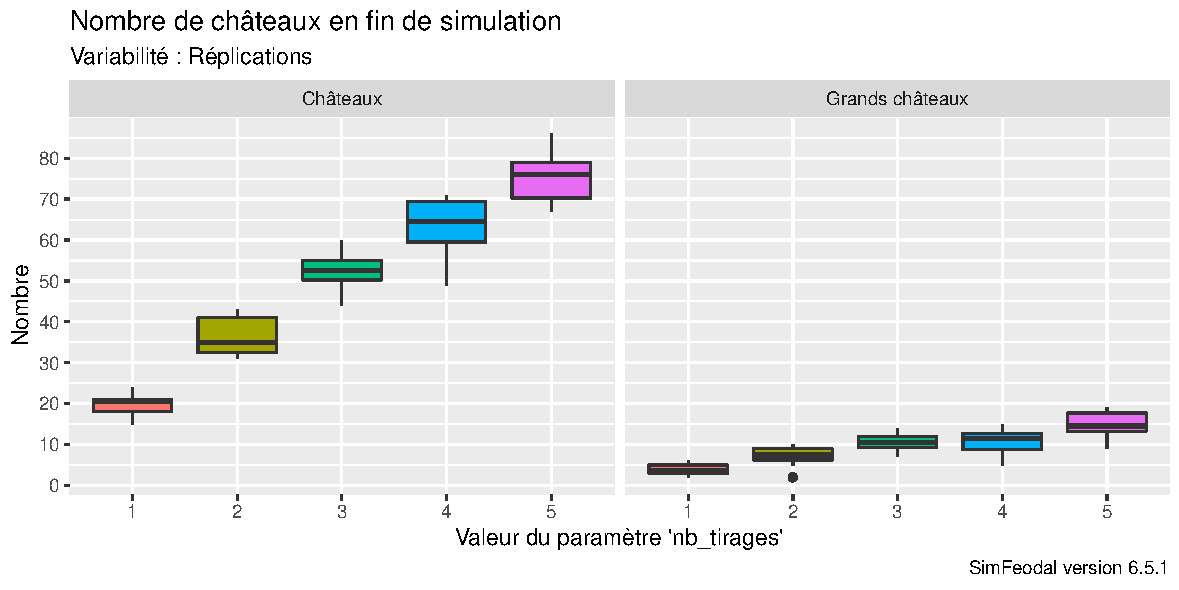
\includegraphics[width=\linewidth]{img/calibrage_nombre_chateaux.pdf}
	\caption[Influence du paramètre \textsf{nb\_tirages} sur le nombre de châteaux.]{Influence du paramètre \textsf{nb\_tirages} sur le nombre de châteaux%\footnotemark.
	}
	\label{fig:calibrage-param-chateaux}
\end{figure}
%\footnotetext{
%	Ce graphique représente une version légèrement différente de la 6.5.1 présentée dans le reste du chapitre.
%	Certaines valeurs de paramètres y sont adaptées au calibrage, fin, des effets de contexte liés aux châteaux.
%}

En jouant sur les différents paramètres associés à la construction d'un château, on obtient un ensemble de valeurs de paramètres qui amènent à la construction d'une quantité régulière de châteaux, dont le nombre en fin de simulation correspond aux données empiriques (\cref{fig:calibrage-chateaux-nb}).

\begin{figure}[H]
	\centering
	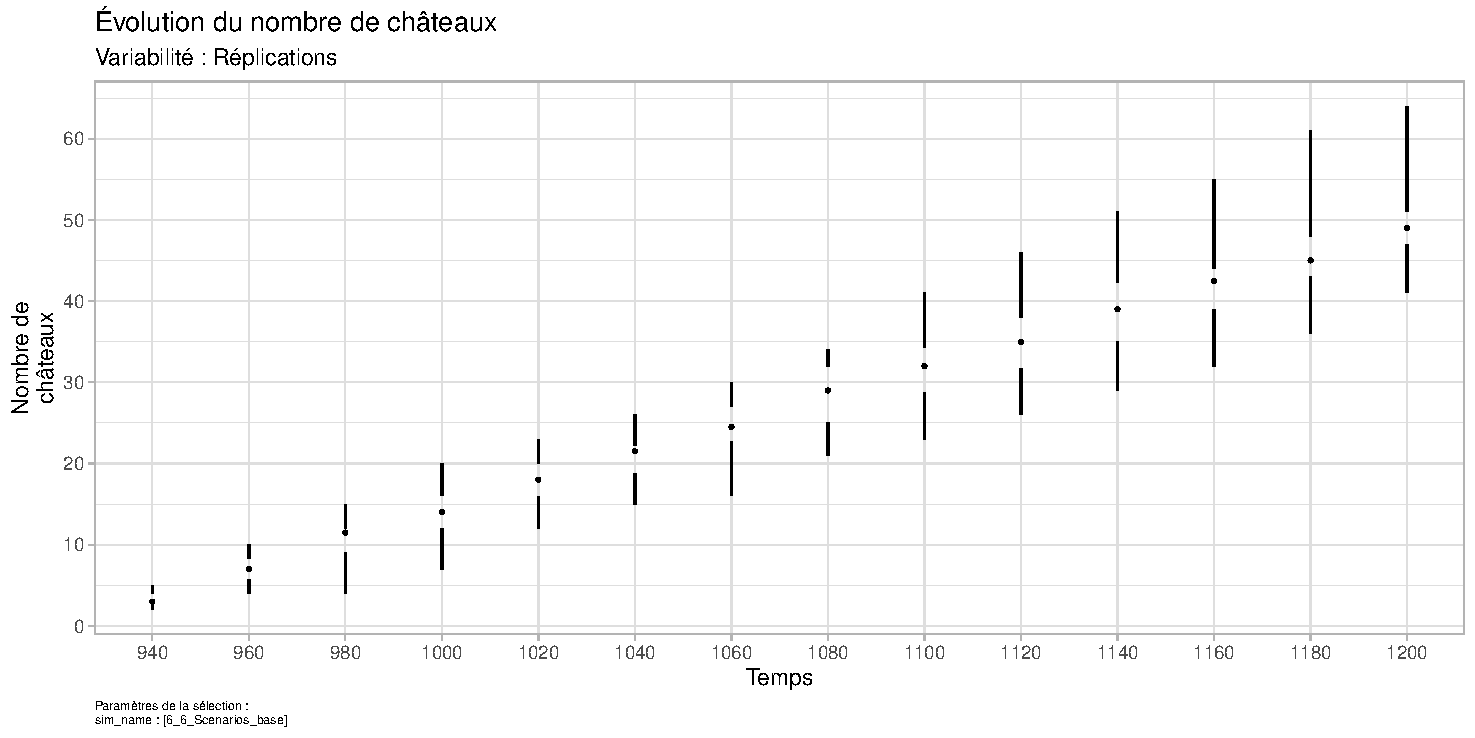
\includegraphics[width=\linewidth]{img/results_6_6/Chateaux_Nb_Haut.pdf}
	\caption[Évolution du nombre de châteaux simulé par le modèle calibré.]{Évolution du nombre de châteaux simulé par le modèle calibré.\\
	\textit{Cet indicateur, comme une large part, est représenté par des \og {\normalfont box-plots} minimalistes\fg{}. Le point central correspond à la médiane, l'espace vide qui entoure ce point à l'intervalle inter-quartile (Q1 et Q3), et les \og moustaches\fg{} représentent les valeurs minimales et maximales.
	}}
	\label{fig:calibrage-chateaux-nb}
\end{figure}

\paragraph{Détail des types des châteaux.}
Le nombre de châteaux n'est toutefois pas la seule valeur empirique sur laquelle on essaie d'ajuster le contexte.
En effet, dans \simfeodal{}, on distingue plusieurs catégories de châteaux, d'une part selon leur importance (gros et petits châteaux), et d'autre part selon le type de seigneurs qui les ont construits (petits ou grands seigneurs).
L'importance des châteaux joue sur leur attractivité vis-à-vis des foyers paysans (un gros château contribue davantage à l'attractivité du pôle d'attraction qui le contient qu'un petit château).
Le type de propriétaire joue quant à lui sur le prélèvement des droits associés : un château construit par un grand seigneur a des zones de prélèvement associées plus larges que celles d'un petit seigneur.

Ces distinctions dans le modèle, d'un niveau de détail supérieur à celui de nombreux mécanismes, sont possibles car elles s'appuient sur des typologies empiriques connues sur la région d'étude.
Leur prise en compte permet d'affiner le contexte spatial dans lequel les foyers paysans évoluent, aussi bien en matière de répulsion (\textit{push}, par le type de constructeur) que d'attraction (\textit{pull}, par les attractivités différenciées).


À la fin de la période, en Touraine, on estime à une dizaine le nombre de \og forteresses\fg{}%\footnote{
%	\hl{Trouver ref. avec Samuel pour distinguer les \og forteresses importantes\fg{} et les \og points fortifiés secondaires\fg{}}
%}.
.
Dans \simfeodal{}, on a donc pu calibrer les paramètres liés à la promotion de châteaux de manière à obtenir 10 gros châteaux (correspondants aux forteresses empiriques) et 40 (50 - 10) petits châteaux en fin de simulation.

On connaît de plus, empiriquement, les seigneurs à l'initiative de la construction des châteaux.
Dans la plupart des cas (de 40 à 45 châteaux sur les 50), ce sont les seigneurs les plus importants : ducs et comtes d'Anjou et de Touraine, représentés dans \simfeodal{} par les grands seigneurs.
Les 5 à 10 châteaux restants sont issus de seigneurs de moindre importance qui ont toutefois acquis une puissance symbolique et militaire bien supérieure à celles des autres petits seigneurs.
Dans \simfeodal{}, on a donc calibré les paramètres régissant les mécanismes de création de châteaux, différenciés pour les grands et petits seigneurs, afin que les valeurs obtenues par simulation soient similaires aux valeurs empiriquement connues.

Les graphiques de la \cref{fig:calibrage-chateaux-composition} présentent les résultats obtenus dans la dernière version de \simfeodal{}.
Ils ne sont pas entièrement satisfaisants, mais résultent d'un compromis entre le calibrage des paramètres vis-à-vis des trois indicateurs que sont le nombre et le type des châteaux, ainsi que le statut de leurs constructeurs.

\begin{figure}[H]
	\centering
	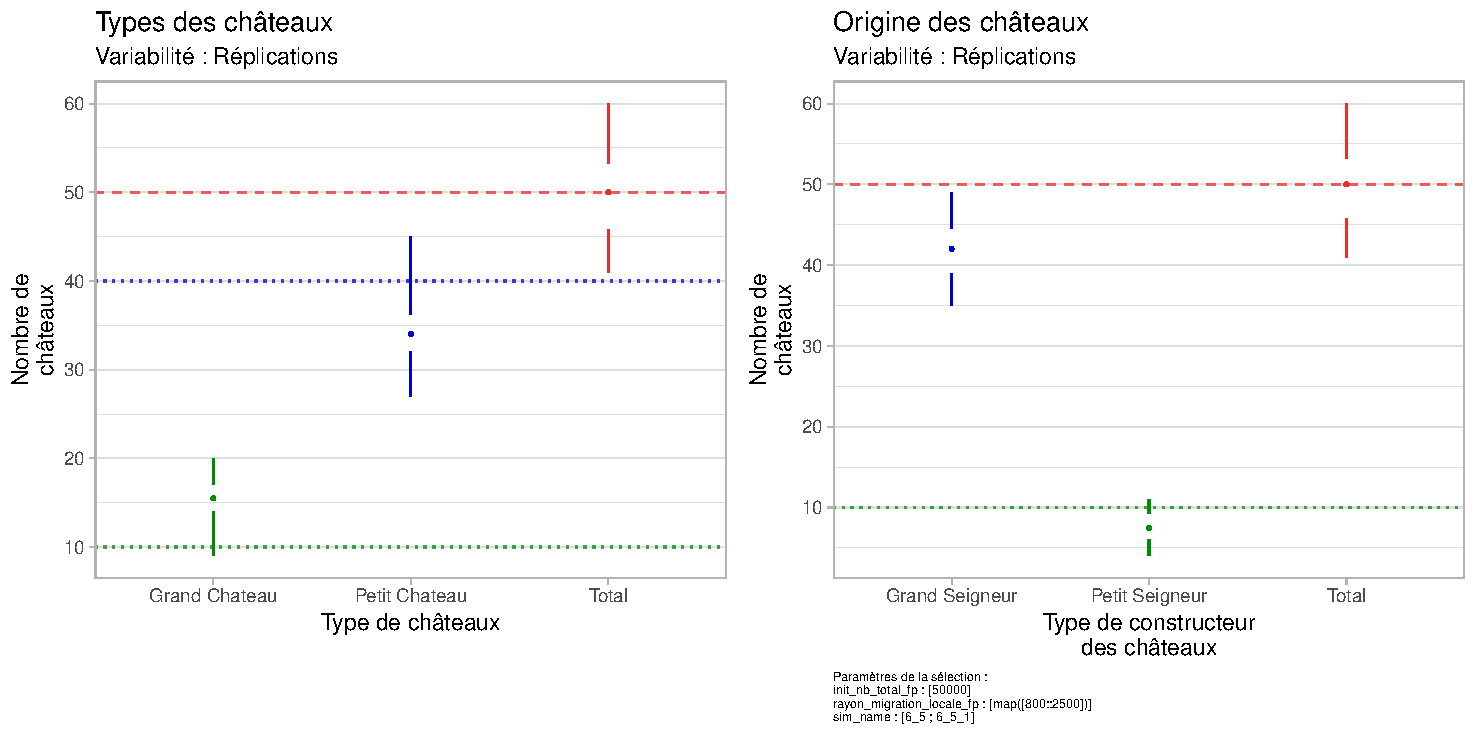
\includegraphics[width=.95\linewidth]{img/Chateaux_Types_condenses.pdf}
	\caption[Détail de la composition des châteaux en fin de simulation à l'issu du calibrage de \simfeodal{}.]{Détail de la composition des châteaux en fin de simulation à l'issu du calibrage de \simfeodal{}.\\
	\textit{Les lignes horizontales en pointillés représentent les objectifs à atteindre, définis selon les connaissances empiriques.}
\smallskip}
	\label{fig:calibrage-chateaux-composition}
\end{figure}


\clearpage
\subsection{Résultats des simulations \label{subsec:resultats}}

%\begin{tcolorbox}[breakable,left=0pt,right=0pt,top=0pt,bottom=0pt,
%	colback=yellow!50,colframe=black,width=\dimexpr\textwidth\relax, 
%	enlarge left by=0mm, boxsep=5pt,arc=0pt,outer arc=0pt]
%Il manque des corrections de Lena, depuis cette intro jusqu'à la figure 6.6 (nombre de pôles et part des agrégats comprenant un pôle).
%Lui redemander la version numérique de sa correction, que je n'ai pas eu pour ce petit bout.
%\end{tcolorbox}

Nous avons largement décrit, dans le \cref{chap:chap3}, les objectifs poursuivis par le modèle et les indicateurs de sortie de simulation employés pour les évaluer.
Pour rappel, ces objectifs peuvent être catégorisés en trois familles, selon les objectifs thématiques qu'ils cherchent à reproduire : 
\begin{itemize}
	\item Polarisation du système de peuplement : le modèle parvient-il à faire émerger une structure polarisée et concentrée de l'habitat, où les foyers paysans sont concentrés dans des agrégats de population plutôt que dispersés comme dans la situation initiale ?
	\item Hiérarchisation du système de peuplement : depuis une situation initiale composée d'une faible hiérarchie dans les agrégats (des \og agglomérations secondaires antiques\fg{} d'une trentaine de foyers et des \og villages\fg{} d'une dizaine de foyers), parvient-on à une structure hiérarchique, proche du modèle log-normal identifié dans la majorité des systèmes de peuplement historiques et contemporains ?
	\item Fixation et dissémination du peuplement : on estime que la population, initialement assez mobile (relativement à la granularité temporelle du modèle, soit tous les 20 ans) tend peu à peu à se fixer.
	Cette fixation, dans des agrégats, s'assortit d'une dispersion à l'échelle de la région modélisée : d'une occupation dispersée et quasi-aléatoire, l'objectif thématique est que les agrégats maillent progressivement l'ensemble du monde simulé.
	Observe-t-on bien ces deux processus dans le déroulement des simulations ?
\end{itemize}

Dans cette partie, nous allons synthétiquement commenter les indicateurs de sortie de simulation issus de la version calibrée (6.6) de \simfeodal{}, en analysant l'écart entre les objectifs attendus, thématiques, et les résultats du modèle.

\begin{mdframed}[backgroundcolor=black!5,footnoteinside=false]
Par soucis de parcimonie et de synthèse, les résultats présentés par la suite ne sont qu'une sélection de l'ensemble des résultats du modèle.
Nous invitons le lecteur à les consulter directement dans l'application \simedb{} d'où ces indicateurs sont extraits.
Le lien suivant permet d'accéder aux résultats spécifiques à la version présentée ici : \href{https://simedb.cura.info/6.6}{https://simedb.cura.info/6.6}
\end{mdframed}

\clearpage
\subsubsection{Résumé global des résultats \label{ssec:results-global}}

Avant de chercher à analyser les résultats du modèle à une échelle fine, le \cref{tab:results-basique} peut déjà synthétiser une bonne part des résultats agrégés, en fin de simulation.
Il rassemble les indicateurs de sortie de simulation quantitatifs, qui décrivent uniquement l'état du modèle en 1200, à la fin de la simulation.


%%%%%%%%%%%%%%%%%%%%%%%%%%%%%%%%%%%%%%%%%%%%
% VERSION SANS LES INDICATEURS DE CONTEXTE %
%%%%%%%%%%%%%%%%%%%%%%%%%%%%%%%%%%%%%%%%%%%%%
\begin{table}[H]
	\captionsetup{singlelinecheck=off}
	\centering
	\small
	\resizebox{\textwidth}{!}{%
	{\renewcommand{\arraystretch}{1.3}%
		\begin{tabular}{|p{3cm}|p{2.2cm}|p{1.5cm}|p{1.5cm}|p{1.5cm}|p{1.5cm}|p{1.5cm}|}
			\hline
			\textbf{Indicateur} & \textbf{Valeur} \textbf{attendue}%\footnotemark
			 & \textbf{Moyenne} & \textbf{Médiane} & \textbf{Q1} & \textbf{Q3} & \textbf{Écart-type} \\ \hline
			\textit{Agrégats} & \textit{200} & 249 & 248 & 244 & 253 & 10.45 \\ \hline
			\textit{Gros châteaux} & \textit{10} & 15 & 15 & 13 & 17 & 2.87 \\ \hline
			\textit{Églises paroissiales} & \textit{300} & 348 & 348 & 338 & 359 & 12.96 \\ \hline
			\textit{Distance moyenne entre églises} & \textit{3 000 m} & 1 459 m & 1 456 m & 1 391 m & 1 537 m & 97 m \\ \hline
			\textit{Part de foyers paysans isolés} & \textit{20 \%} & 30 \% & 30 \% & 30 \% & 30 \% & 0.8 \% \\ \hline
			\textit{Augmentation de la charge fiscale des foyers paysans} & \textit{×3} & ×2.4 & ×2.4 & ×2.4 & ×2.5 & ×0.03 \\ \hline
	\end{tabular}}}
	\caption{Valeurs des indicateurs numériques en fin de simulation.}
	\label{tab:results-basique}
\end{table}
%\footnotetext{Objectif en fin de simulation}

On y constate en premier lieu que les ordres de grandeur sont plutôt respectés, à l'exception peut-être de la distance entre églises paroissiales\footnote{
	La distance moyenne simulée	est ainsi de 1459m, c'est-à-dire deux fois moindre que les estimations empiriques.
	Notons que cela s'explique notamment par le nombre trop élevé d'églises paroissiales, et par la difficile constitution de cet indicateur : les données empiriques concernent surtout les paroisses rurales, alors que l'on tient ici compte de l'ensemble des églises paroissiales.
	Les églises paroissiales urbaines, très proches les unes des autres, tirent ainsi considérablement la moyenne des distances à la baisse.
	Il est difficile, dans le modèle, de différencier les églises paroissiales rurales et urbaines, et on ne peut donc obtenir un indicateur de sortie directement comparable aux données empiriques.
}.

Concernant les autres indicateurs, on peut noter qu'ils sont en général supérieurs aux valeurs attendues, ce qui est d'autant plus significatif que la variabilité de ces indicateurs est faible (les médianes et quartiles sont assez proches de la moyenne, et l'écart-type est faible relativement aux grandeurs considérées).
Le nombre d'agrégats et d'églises paroissiales simulés dépasse d'une cinquantaine les valeurs empiriques correspondantes.
La part de foyers paysans isolés en fin de simulation est trop importante de 10\%, quand bien même l'intervalle de confiance empirique est assez flou.

Le nombre de gros châteaux dépasse significativement l'objectif, comme on a pu le constater dans la \cref{fig:calibrage-chateaux-composition} (gauche), mais ajuster davantage cette valeur aux quantités empiriques déstabilise d'autres éléments du modèle.

Le dernier indicateur, l'augmentation de la charge fiscale des foyers paysans, est quant à lui assez satisfaisant : il est certes plus faible que l'objectif empirique fixé (augmentation de 2.4 au lieu de 3 de la charge fiscale moyenne entre le début et la fin de la simulation), mais dans le cas de cet objectif empirique difficile à estimer, cette valeur nous paraît suffisante.

Dans la suite de cette partie, nous menons une analyse plus fine des résultats du modèle, en observant de manière plus précise les valeurs des indicateurs de sortie de simulation qui caractérisent les \og trois familles\fg{} d'objectifs thématiques : polarisation, hiérarchisation et fixation-dissémination.

\subsubsection{Capacité du modèle à simuler la polarisation des foyers paysans}

Les résultats mettent en évidence une forte concentration des foyers paysans, dont la part de foyers isolés diminue de manière importante, d'environ 90\% à 30\% en fin de simulation (\cref{fig:results-concentration-fp}).

\begin{figure}[H]
	\centering
	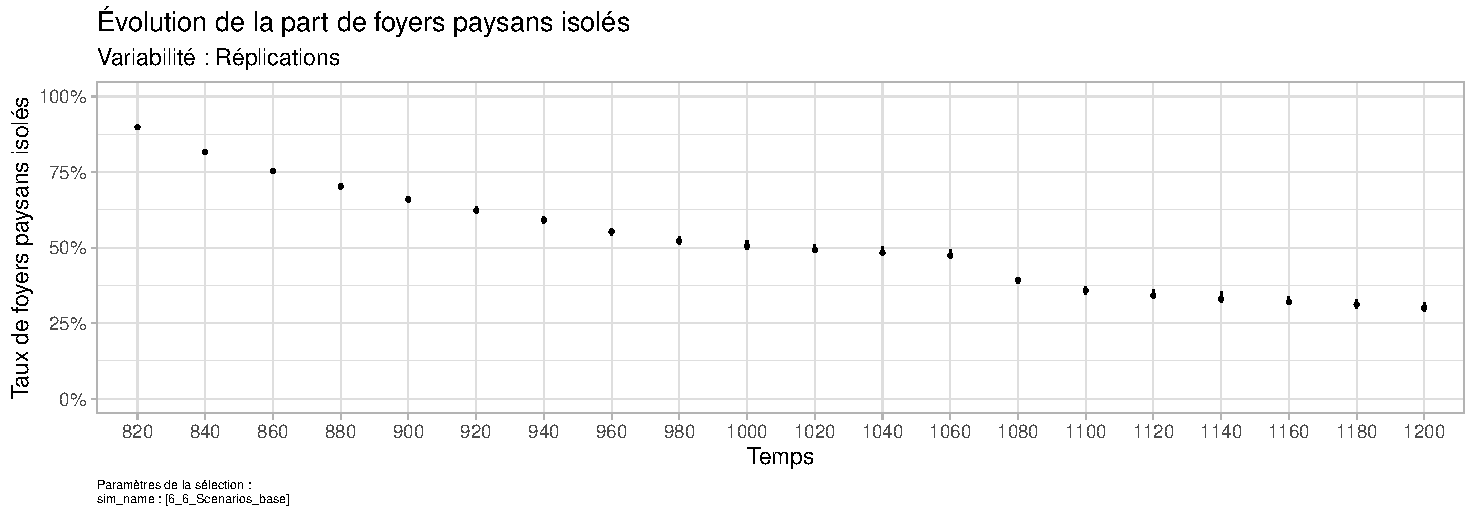
\includegraphics[width=\linewidth]{img/results_6_6/FP_Concentration_Haut.pdf}
	\caption{Concentration des foyers paysans.}
	\label{fig:results-concentration-fp}
\end{figure}

Cette diminution paraît assez régulière, en dépit d'une légère rupture de tendance entre 1060 et 1080, période qui correspond dans le modèle à une évolution du seuil de satisfaction religieuse.
Notons que parmi les 20 réplications étudiées, cet indicateur se montre extrêmement stable, les marques visuelles de variabilité étant à peine visibles.

\begin{figure}[H]
	\centering
	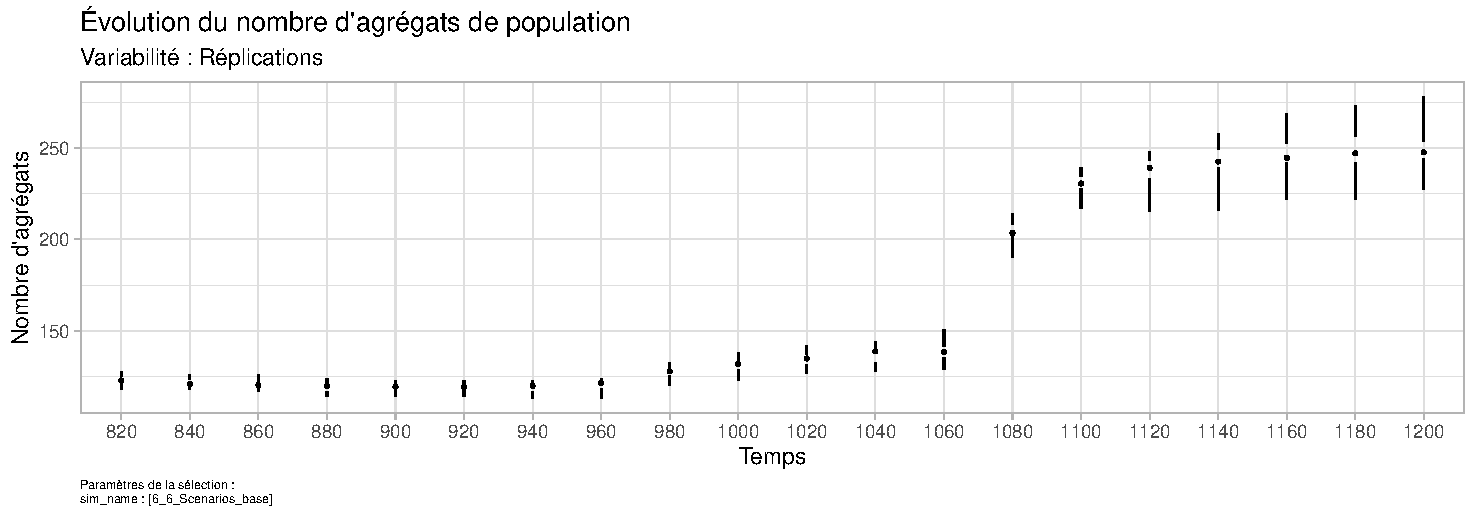
\includegraphics[width=\linewidth]{img/results_6_6/Agregats_Nb_Haut.pdf}
	\caption{Nombre d'agrégats.}
	\label{fig:results-nb-agregrats}
\end{figure}

La concentration des foyers paysans s'effectue à destination d'un nombre croissant d'agrégats (\cref{fig:results-nb-agregrats}).
Dans l'évolution de ce nombre, on constate un effet de seuil important entre 1060 et 1080 (pour les mêmes raisons que l'augmentation de la concentration), mais aussi, un premier changement de tendance entre 940 et 960 d'ampleur moindre.
Ces deux paliers caractérisent les trois régimes repérés empiriquement, c'est-à-dire une augmentation lente, suivie d'une augmentation rapide et enfin une stabilisation du nombre d'agrégats.

À la différence d'une simple concentration du peuplement, la polarisation implique que des éléments (des pôles) jouent un rôle d'attracteur, et que la concentration s'effectue donc à proximité de ces pôles.

Dans \simfeodal{}, on cherche donc d'une part à ce que les foyers paysans se concentrent et forment des agrégats, et d'autre part à ce que ces agrégats se constituent autour des pôles d'attraction constitués par les agents attracteurs du modèle (églises paroissiales, châteaux et agrégats dotés de communautés paysannes).
Pour savoir si le modèle parvient bien à reproduire le fait stylisé qu'est la polarisation du peuplement, on mobilise donc des indicateurs relatifs à la quantité de pôles et à leur localisation.

Dans cette version du modèle, on constate bien une croissance du nombre de pôles (\cref{fig:results-nb-poles-agregats}-a), assez semblable à celle des agrégats en termes de rythme et de valeur.
Les valeurs atteintes (environ 250 pôles en fin de simulation) sont très satisfaisantes, particulièrement au regard des résultats des premières versions du modèle.

\begin{figure}[H]
	\centering
	\hspace{5pt}
	\subfloat[][Pôles d'attraction.]{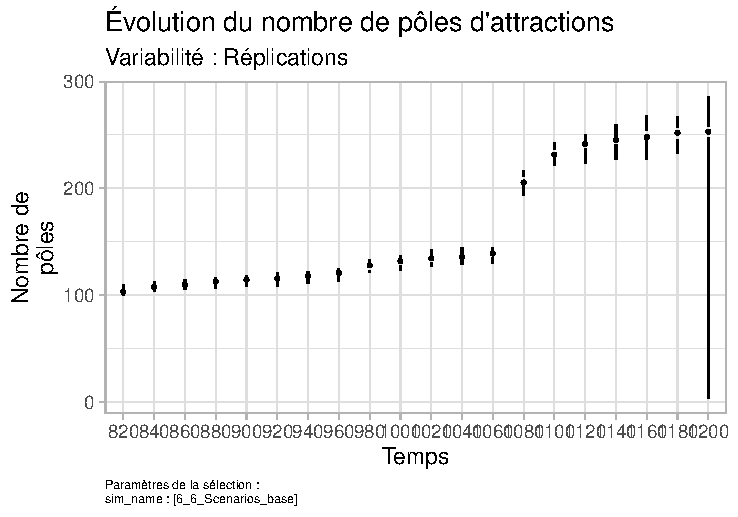
\includegraphics[width=.49\linewidth]{img/results_6_6/Poles_Nb_Haut.pdf}}
	\subfloat[][Agrégats avec pôle.]{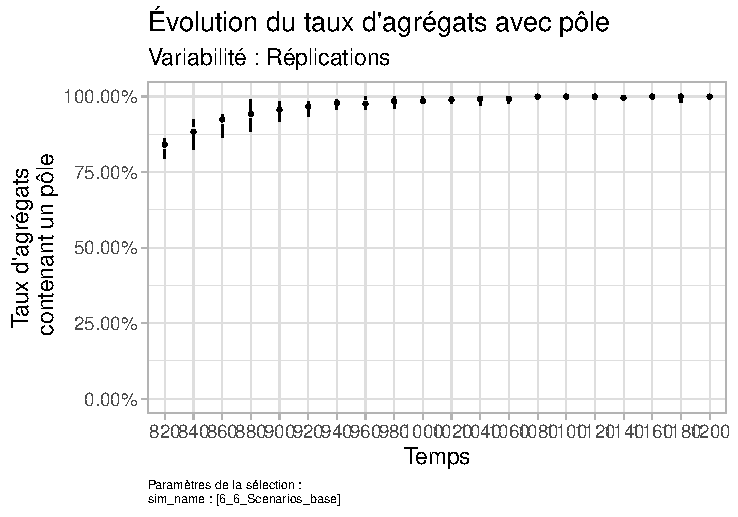
\includegraphics[width=.49\linewidth]{img/results_6_6/Agregats_Poles_Haut.pdf}}
	\caption[Nombre de pôles et part des agrégats comprenant un pôle.]{Nombre de pôles et part des agrégats comprenant un pôle.}
	\label{fig:results-nb-poles-agregats}
\end{figure}

La \cref{fig:results-nb-poles-agregats}-b présente elle-aussi des résultats satisfaisants, qui viennent préciser l'analyse précédente.
Cette figure présente l'évolution du taux d'agrégats qui sont situés dans un pôle d'attraction.
On remarque que ce taux augmente très rapidement pour ensuite se maintenir autour de 100\% : cela signifie que tous les agrégats sont situés dans un pôle, et donc que les agrégats se sont bien formés autour de pôles d'attraction plutôt que de manière purement dispersée.
Cette figure constitue ainsi un des indices montrant que \simfeodal{} parvient bien à reproduire le processus de polarisation tel qu'observé empiriquement.

Les cartes de la \cref{fig:results-carte-agregats_poles} permettent de noter que le semis des pôles se confond spatialement avec celui des agrégats, ce qui amène un élément d'interprétation supplémentaire : les agrégats sont bien constitués dans des pôles (paragraphe précédent), mais en plus, tous les pôles semblent contenir un ou des agrégats.
Le modèle fait donc émerger une quasi-équivalence entre pôles et agrégats, quasi-équivalence que l'on retrouve chez \textcite[27-28]{le1976eglise}, en assimilant les pôles à leurs seules églises : \og Le village appelle l'église. [...] L'église fait naître le village.\fg{}.
\clearpage

%Ces agrégats et les pôles correspondant sont bien plus dispersés dans l'espace du modèle que dans la version 0, et on constate, au moins visuellement, que le semis des pôles se confond avec celui des agrégats (\cref{fig:results-carte-agregats_poles}).
%Sur ces cartes, on constate une occupation importante de l'espace, largement due à une population bien supérieure en version 6.6 (40 000 foyers paysans, contre 4 000 en version 0), mais on remarque toutefois sur la troisième carte, lissée, qu'en dépit d'un semis visiblement homogène, des zones de plus forte densité sont présentes.

\begin{figure}[H]
	\centering
	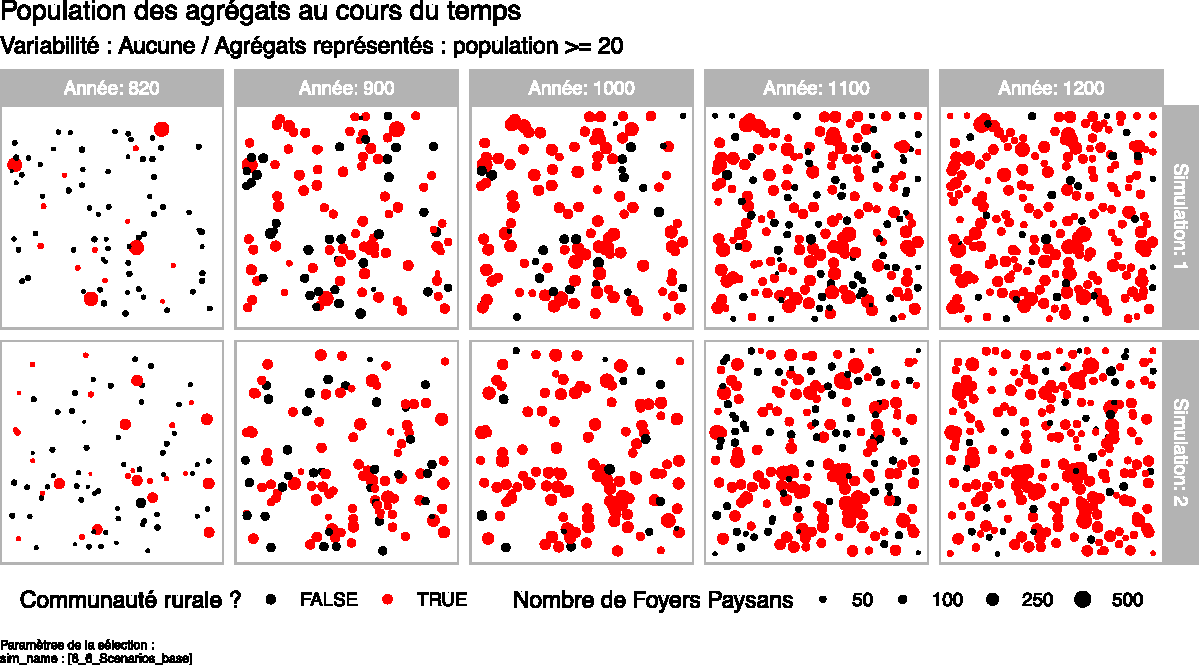
\includegraphics[width=\linewidth]{img/results_6_6/Agregats_Carte_Haut.pdf}
	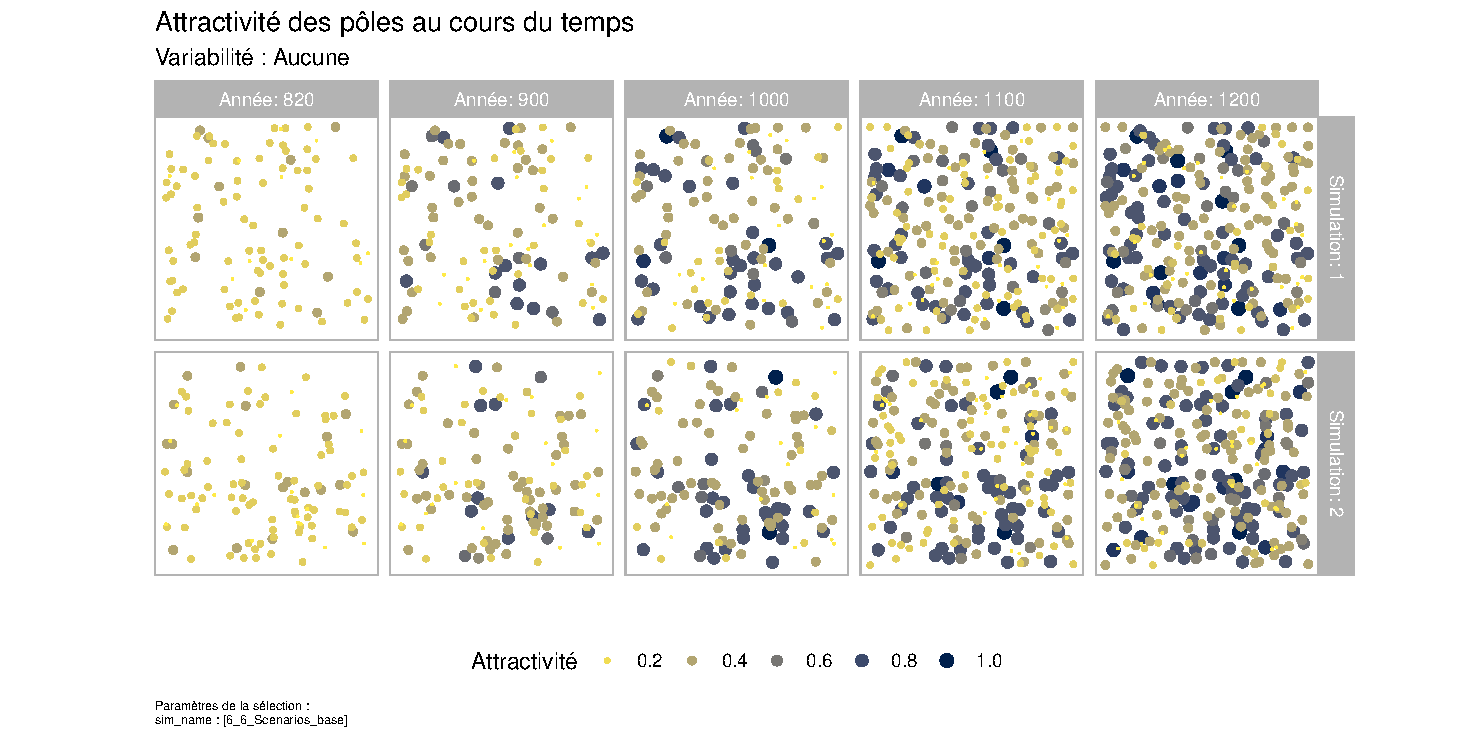
\includegraphics[width=\linewidth]{img/results_6_6/Poles_Carte_Haut.pdf}
	\caption[Dispersion spatiales des agrégats et pôles.]{Dispersion spatiales des agrégats et pôles.\\
	\textit{N.B. : Les simulations \og 1\fg{} et \og 2\fg{} sont deux réplications d'une même expérience. Leur intitulé n'a aucun autre sens que d'en permettre la différenciation.}}
	\label{fig:results-carte-agregats_poles}
\end{figure}

\bigskip
\paragraph[Conclusion intermédiaire]{}
Sur le plan de la polarisation d'ensemble des foyers paysans au sein d'agrégats de population, les résultats du modèle montrent que \simfeodal{} est entièrement capable de reproduire les attendus.
La valeur finale issue des simulations est certes légèrement inférieure à l'objectif, mais tous les ordres de grandeurs et surtout les rythmes estimés correspondent largement aux estimations issues des connaissances expertes.

\clearpage
\subsubsection{Capacité du modèle à simuler la hiérarchisation du système de peuplement}

Les dernières figures étudiées montraient une forte hétérogénéité dans la taille des agrégats (un agrégat est créé dès 5 foyers paysans, et la légende de la première série de cartes -- dispersion des agrégats -- s'étend entre 50 et 500 foyers), ce qui constitue déjà un indice sur le niveau de hiérarchisation de ces concentrations locales de foyers paysans.

Comme indiqué dans le chapitre 3, il est difficile d'avoir des mesures précises de la distribution statistique attendue dans le système de peuplement.
Les différentes sources historiques divergent aussi bien sur les quantités absolues que sur la forme des distributions.
Ces sources s'accordent en revanche sur une nette hiérarchisation, avec une distribution qui doit tendre vers les formes log-normales dont l'on retrouve l'existence dans les sociétés contemporaines.

%\begin{table}[H]
%	\captionsetup{singlelinecheck=off}
%	\centering
%	\small
%	{\renewcommand{\arraystretch}{1.3}%
%		\begin{tabular}{p{2.5cm}|p{1.5cm}|p{1.5cm}|p{1.5cm}|p{1.5cm}|p{1.5cm}|p{1.5cm}|}
%			\cline{2-7}
%			& \multicolumn{6}{c|}{\textbf{Nombre de foyers paysans}} \\
%			 & \textbf{<100} & \textbf{101-200} & \textbf{201-300} & \textbf{301-400} &\textbf{ 401-600} & \textbf{>600} \\ \hline
%			 \multicolumn{1}{|c|}{Nombre moyen} & 142 & 78 & 18 & 7 & 4 & 2 \\ \hline
%			 \multicolumn{1}{|c|}{Taux moyen} & 56.8\% & 31.4\% & 7\% & 2.9\% & 1.6\% &<0.1\% \\ \hline
%			 \rowcolor{yellow} \multicolumn{1}{|c|}{\textit{Objectif (taux)}} & \textit{?} & \textit{?} & \textit{?} & \textit{?} & \textit{?} & \textit{?}\\ \hline	
%	\end{tabular}}
%	\caption[Distribution des agrégats par classe de taille en fin de simulation.]{Distribution des agrégats par classe de taille en fin de simulation. \hl{Ne conserver que si Cécile arrive à trouver, pour l'article anglais, une validation des objectifs par EZR/SL.}}
%	\label{tab:distrib-population-agregats}
%\end{table}

\begin{figure}[H]
	\centering
	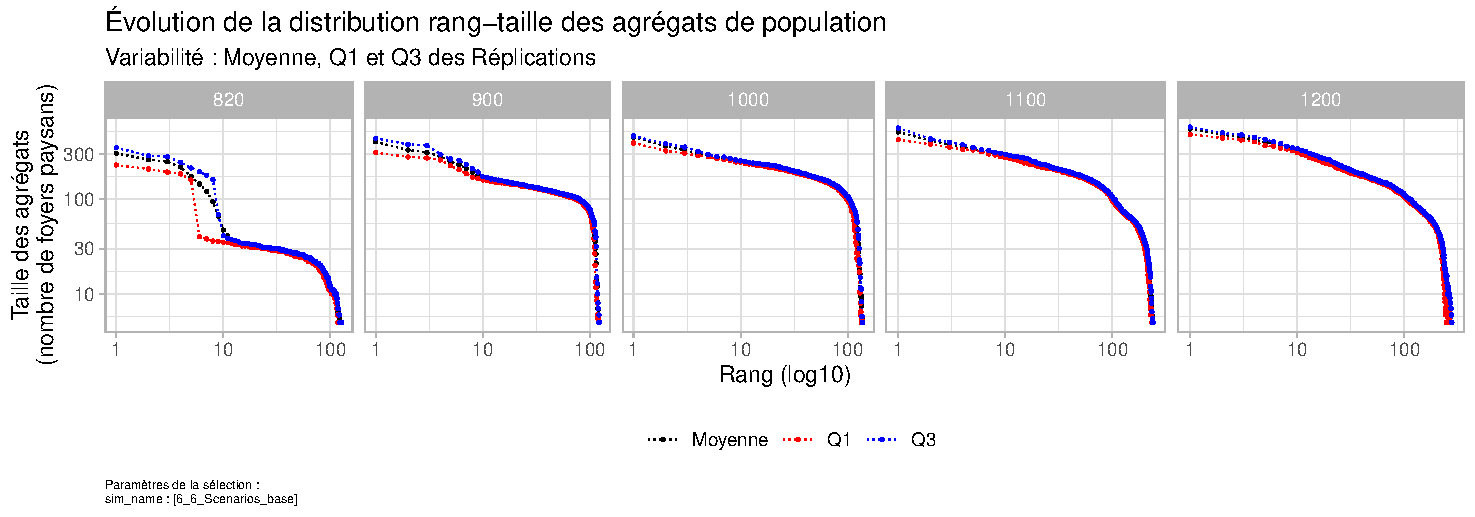
\includegraphics[width=\linewidth]{img/results_6_6/Agregats_RT_Haut.pdf}
	\caption[Hiérarchie des agrégats]{Organisation hiérarchique des agrégats.}
	\label{fig:results-rt-agregats}
\end{figure}

La \cref{fig:results-rt-agregats} montre une claire hiérarchisation des agrégats : la courbe se \og redresse\fg{} au cours de la simulation, marque d'une pente croissante.
Les valeurs absolues augmentent aussi : les plus gros agrégats voient leur population croître.
Le \og coude\fg{} dans la courbe, qui correspond à la longue traîne de petits agrégats, se réduit.
%Contrairement à la version 0 du modèle, la croissance de tous les agrégats semble constante, et on ne remarque pas, visuellement, les tendances à l'éclatement des gros agrégats qui caractérisaient la hiérarchie de cette version.

En parallèle de cette nette hiérarchisation des agrégats, les graphiques de la \cref{fig:results-rt-poles} permettent de constater une toute aussi nette hiérarchisation des pôles.
Cela n'est pas surprenant dans la mesure où on a vu qu'agrégats et pôles se confondaient, ce qui constitue en soi un résultat satisfaisant.
La hiérarchie des pôles peut aussi être lue dans la composition des pôles en attracteurs.
Dans l'ensemble, plus un pôle contient d'agents-attracteurs, plus il est susceptible d'être attractif.
Les pôles sont ainsi constitués d'agents-attracteurs, chacun dotés d'une valeur d'attractivité, et c'est donc leur combinaison qui défini l'attractivité des pôles.
\clearpage

\begin{figure}[H]
	\centering
	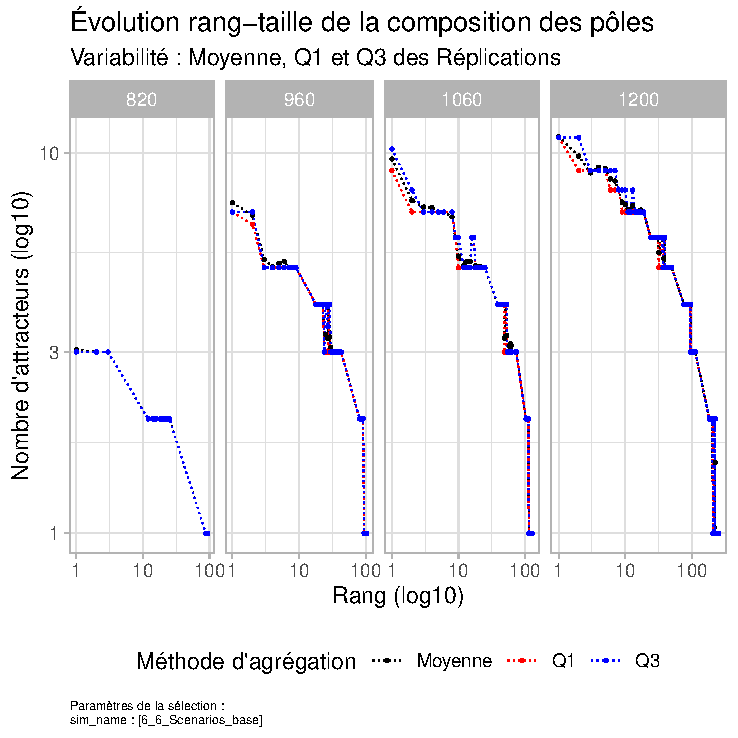
\includegraphics[width=.405\linewidth]{img/results_6_6/Poles_RT_Haut.pdf}
	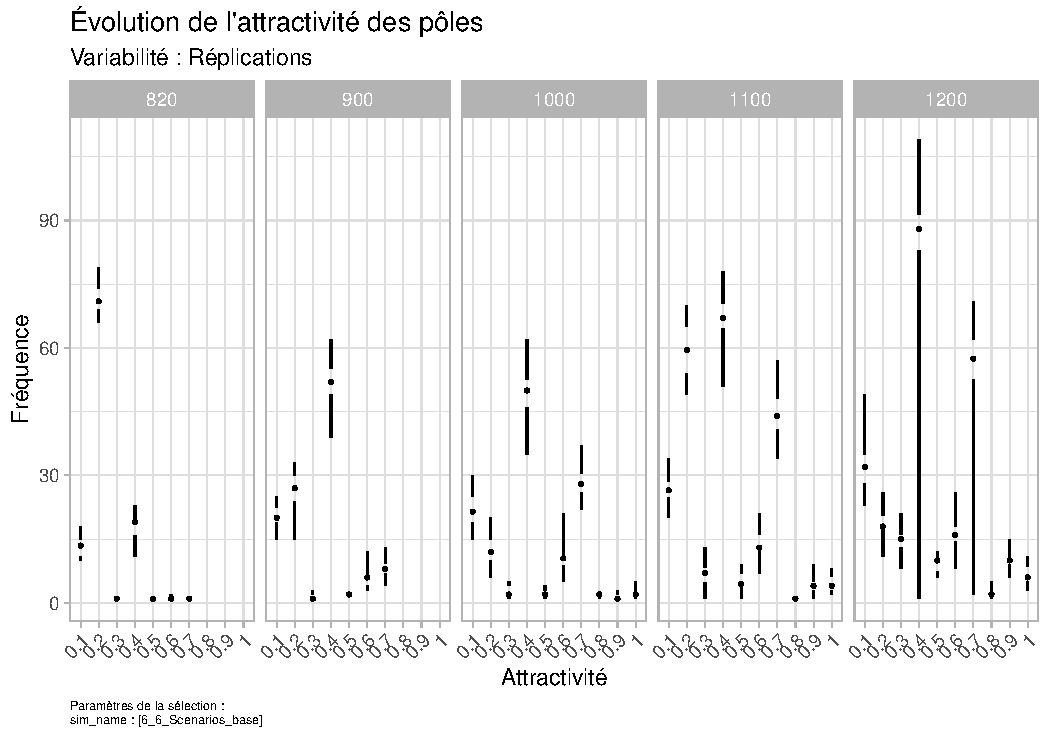
\includegraphics[width=.58\linewidth]{img/results_6_6/Poles_Attrac_Haut.pdf}
	\caption[Hiérarchie des pôles.]{Organisation hiérarchique des pôles.}
	\label{fig:results-rt-poles}
\end{figure}

La mesure représentée dans la figure de gauche -- le nombre d'attracteurs de chaque pôle -- est beaucoup plus \og discrète\fg{} que le nombre de foyers paysans des agrégats.
Il y a moins de modalités (de un à une dizaine d'attracteurs, contre de 5 à plus de 500 foyers paysans), donc moins d'effets possibles de coudes.
Ce graphique communique donc plus lisiblement, visuellement, la forte hiérarchisation des pôles.
Comme le nombre maximum d'attracteur augmente régulièrement (environ 3 en début de simulation contre plus de 10 à la fin), on peut dire que dans le modèle, cette hiérarchisation est dûe à une croissance plus que proportionnelle des pôles les plus importants et non à une croissance équitablement répartie.
Par exemple, en fin de simulation, sur les 250 pôles, moins de la moitié est composée de plus de trois attracteurs.

En cela, le modèle reproduit bien l'apparition d'une tête de hiérarchie urbaine, qui trouve une correspondance empirique dans les villes (Amboise, Loches, Chinon, etc.) de la région d'étude, organisées autour de châteaux et composées de multiples églises paroissiales.
La \cref{fig:results-rt-poles}-b montre aussi cette hiérarchisation : elle met en évidence un glissement des modalités d'attraction depuis une valeur de 0.2 (deux églises paroissiales) à un double mode à 0.4 (deux églises et une communauté) et 0.7 (plusieurs églises, un château, une communauté, etc.).


Un dernier élément du modèle en lien avec la hiérarchisation du peuplement est la hiérarchie des paroisses.
On peut extraire deux types de comportements attendus à partir des connaissances empiriques.

\begin{itemize}
	\item En premier lieu, une large majorité des paroisses, que l'on pourrait nommer \og rurales\fg{}, sont peu fréquentées et visent surtout à une desserte équitable de la population.
	Un paroissien ne devait ainsi pas avoir à effectuer plus d'une heure de marche pour se rendre dans son église paroissiale.
	\item En second lieu, les paroisses \og urbaines\fg{} desservent un nombre de paroissiens bien supérieur à celui des paroisses rurales.
	D'après les connaissances expertes, ce nombre reste largement inférieur au millier de paroissiens, puisque de nouvelles paroisses urbaines étaient créées pour décharger les églises paroissiales trop fréquentées.
\end{itemize}
\clearpage

En agrégeant ces types de paroisses, le fait stylisé que l'on cherche à reproduire dans le modèle serait donc d'avoir une distribution composée de deux tendances : une tête de hiérarchie desservant un grand nombre de paroissiens, mais avec une faible hiérarchisation interne (paroisses urbaines), et une très longue traine, cette-fois ci plus hiérarchisée et desservant beaucoup moins de paroissiens (paroisses rurales).


Dans la \cref{fig:results-rt-paroisses}, on constate que le modèle semble reproduire ce type de distribution : on y remarque bien une courbe caractérisée par une double tendance.
Le haut de la hiérarchie présente une pente faible, signe d'une homogénéité importante entre 100 et 300 paroissiens, et est nettement séparé d'une longue traîne, graphiquement presque verticale, inférieure à 100 paroissiens dans le dernier siècle simulé.
Le nombre maximum de paroissiens diminue au cours de la simulation, passant de plus de 1000 à environ 300.

\begin{figure}[H]
	\centering
	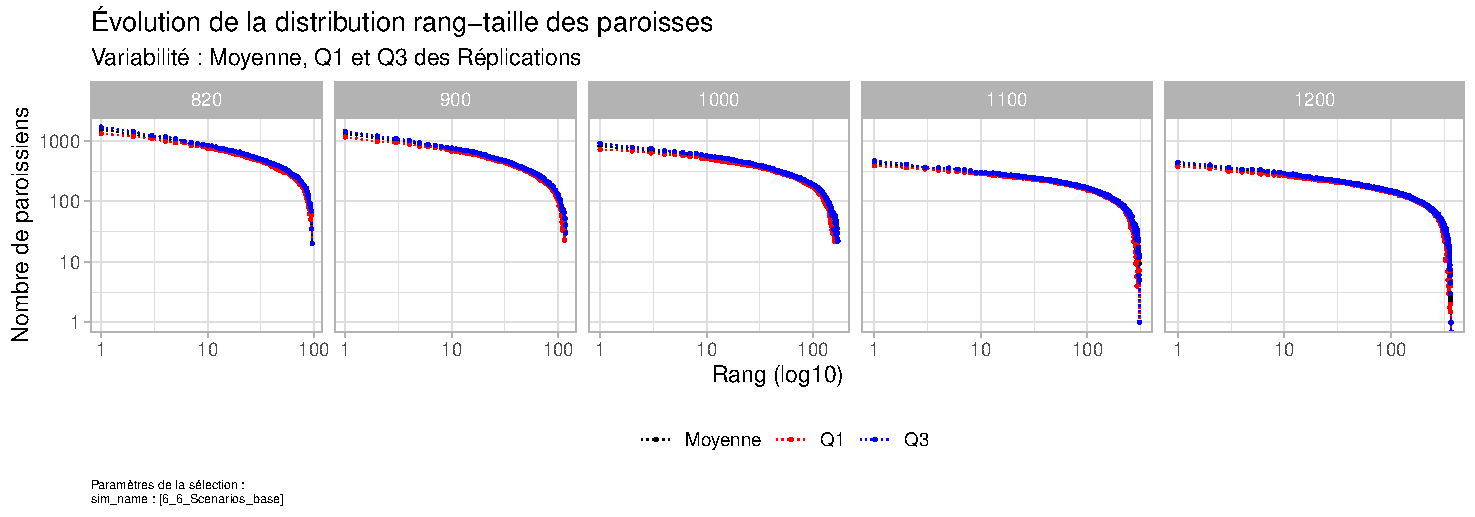
\includegraphics[width=\linewidth]{img/results_6_6/Paroisses_RT_Haut.pdf}
	\caption{Organisation hiérarchique des paroisses.}
	\label{fig:results-rt-paroisses}
\end{figure}

En regardant des indicateurs plus détaillés (\cref{fig:results-paroisses-hierarchie}), on peut remarquer que cela correspond en fait à une forte homogénéisation dans les intervalles de 50 à 200 paroissiens (51-100 et 101-200) qui deviennent en fin de simulation le mode principal de la distribution.
Cet intervalle correspond aux paroisses rurales qui contiennent quelques agrégats ruraux de taille moyenne à faible (\cref{fig:results-rt-agregats}).

\begin{figure}[H]
	\centering
	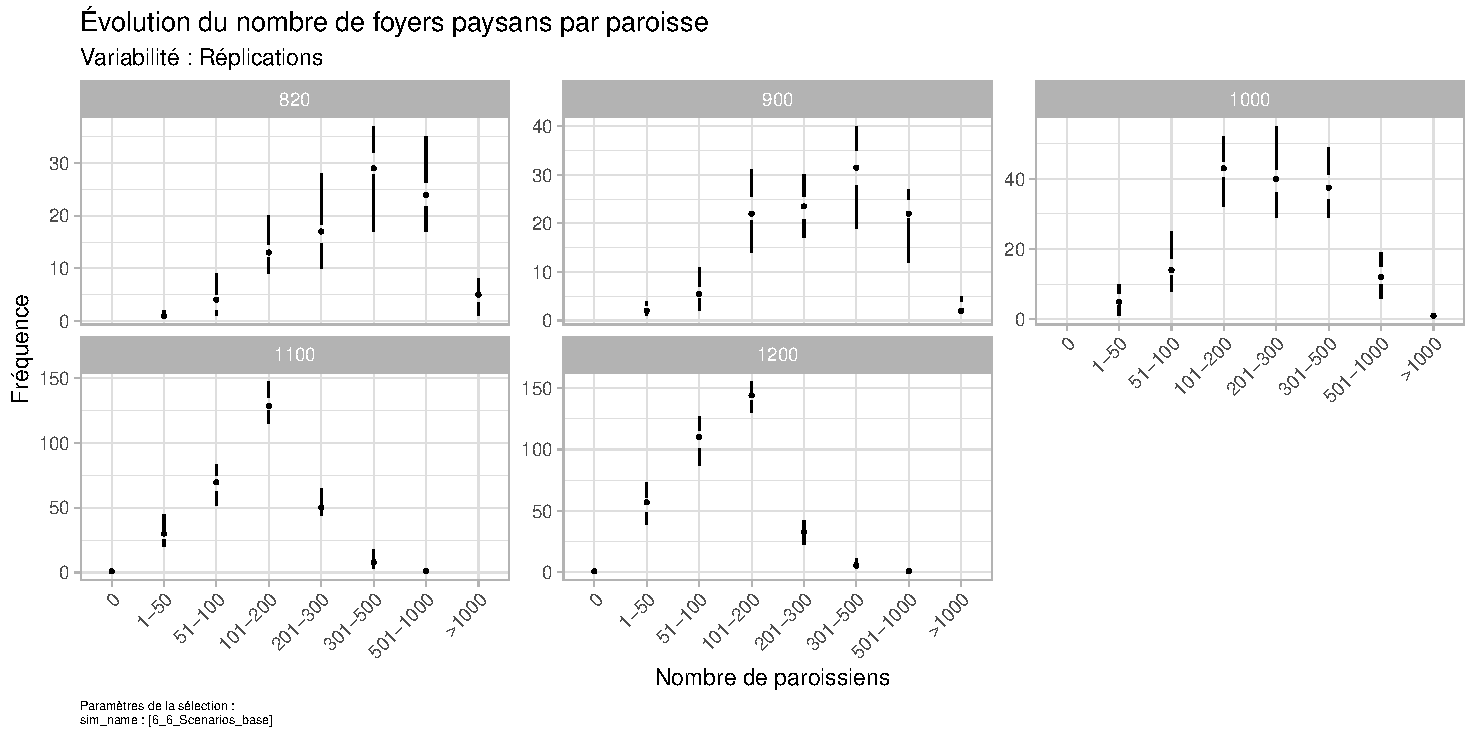
\includegraphics[width=\linewidth]{img/results_6_6/Paroisses_Compo_Haut.pdf}
	\caption{Détail de la distribution hiérarchique des paroisses.}
	\label{fig:results-paroisses-hierarchie}
\end{figure}
\clearpage

\simfeodal{} parvient donc bien à reproduire la double-densification du maillage paroissial.
En milieu rural, le nombre de paroisses augmente jusqu'à assurer une desserte équitable des foyers paysans qui dans le même temps ont tendance à se concentrer, et en milieu urbain, le nombre de paroisses augmente aussi jusqu'à uniformiser le nombre de foyers paysans par paroisse entre 200 et 300.

\medskip
\paragraph[Conclusion intermédiaire]{}
Dans l'ensemble, \simfeodal{} montre une bonne capacité à reproduire la hiérarchisation du système de peuplement.
Avec les informations dont l'on dispose pour évaluer le modèle, on ne peut qu'être satisfait des tendances présentes dans cette version calibrée de \simfeodal{}.
Le modèle reproduit en effet bien les faits stylisés estimés, même si ces derniers sont formalisés de manière plus floues que par exemple le phénomène de polarisation.
Cette incertitude est due à la faiblesse de la documentation empirique sur ces questions thématiques : il s'avère difficile d'avoir une estimation des populations à cette période féodale, ainsi la forme précise de distribution de ces populations est encore plus difficile à estimer.
À ce stade de maturité du modèle, il faudrait sans doute collecter de nouvelles sources historiques pour pouvoir raffiner le comportement du modèle, ou au moins, départager des simulations présentant de légères variations au niveau des indicateurs analysés dans cette sous-partie.

\subsubsection{Capacité du modèle à simuler la fixation et la dissémination du peuplement \label{sssec:fixation-dissemination}}

Dans ce dernier objectif thématique, on cherche à vérifier si le modèle parvient bien à reproduire le double processus de fixation des foyers paysans et de dissémination des peuplements dans l'espace.

Dans le modèle, ces processus devraient s'exprimer sous la forme d'un accroissement des migrations (restructuration) suivi d'une diminution nette (fixation).
Au niveau d'observation des agrégats, on devrait observer une couverture croissante, de plus en plus dense, du monde simulé.

\paragraph{Fixation des foyers paysans.}

\begin{figure}[H]
	\centering
	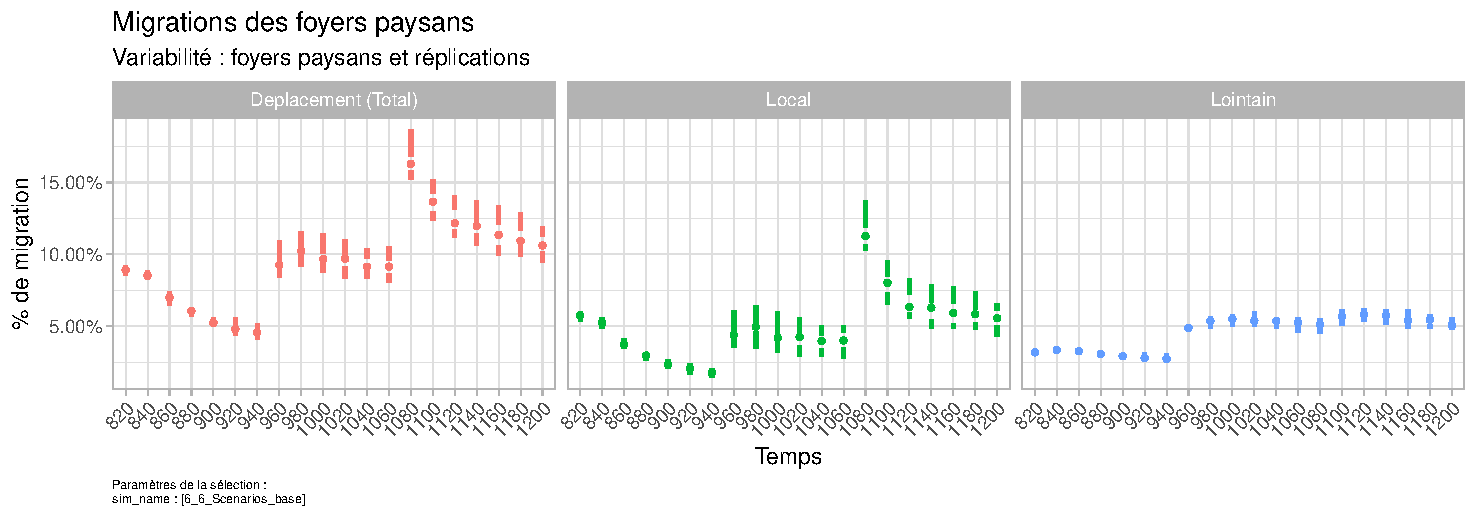
\includegraphics[width=\linewidth]{img/results_6_6/FP_TypeDeplacements_Haut.pdf}
	\caption{Migration des foyers paysans.}
	\label{fig:results-fp-migrations-base}
\end{figure}

La \cref{fig:results-fp-migrations-base} illustre l'évolution des migrations, selon leur type (locale ou lointaine, cf. \cref{meca-migration}) au cours du temps.
On y constate que le modèle produit un motif spécifique, composé de trois phases :
\begin{itemize}
	\item Avant 960, les migrations diminuent de manière régulière, depuis près de 10\% de migrations (total) jusqu'à 5\%.
	Dans le modèle, cette période correspond aux premiers regroupements de foyers paysans.
	Ces derniers, initialement isolés, rejoignent des pôles locaux (églises rurales par exemple) et y constituent ainsi de petits agrégats ruraux locaux.
	Ils se fixent dans ces agrégats car il n'y pas encore véritablement de motif d'insatisfaction (religieuse ou de protection du moins).
	\item En 960, deux éléments exogènes viennent perturber le système : l'augmentation de la pression religieuse (diminution des seuils de distance aux églises) et de la pression de protection (nécessité de s'approcher des châteaux).
	En conséquence, le nombre de migrations bondit et retrouve son niveau de début de simulation (environ 10\%).
	Le besoin de protection augmente régulièrement à cette période, et les foyers paysans sont donc sans cesse amenés à migrer, ce qui explique que ce niveau de migration semble stable jusqu'à la fin de cette deuxième phase%.\footnote{
		. Si de nouveaux éléments exogènes ne venaient pas à nouveau perturber le système après 1060, le niveau de migration diminuerait à son tour, comme avant 960.
	%}.
	\item Une nouvelle rupture survient en 1060, là encore en raison d'une augmentation, exogène, de la pression religieuse (les seuils acceptables de distance à l'église paroissiale diminuent encore jusqu'à devenir très restreints).
	À nouveau, les migrations (uniquement locales cette fois-ci) augmentent de manière abrupte, et, comme dans la première phase, tendent ensuite à diminuer : le niveau maximal d'exigences (religieuse, de protection) est atteint, et les migrations des foyers paysans y pallient.
\end{itemize}

\begin{figure}[H]
	\centering
	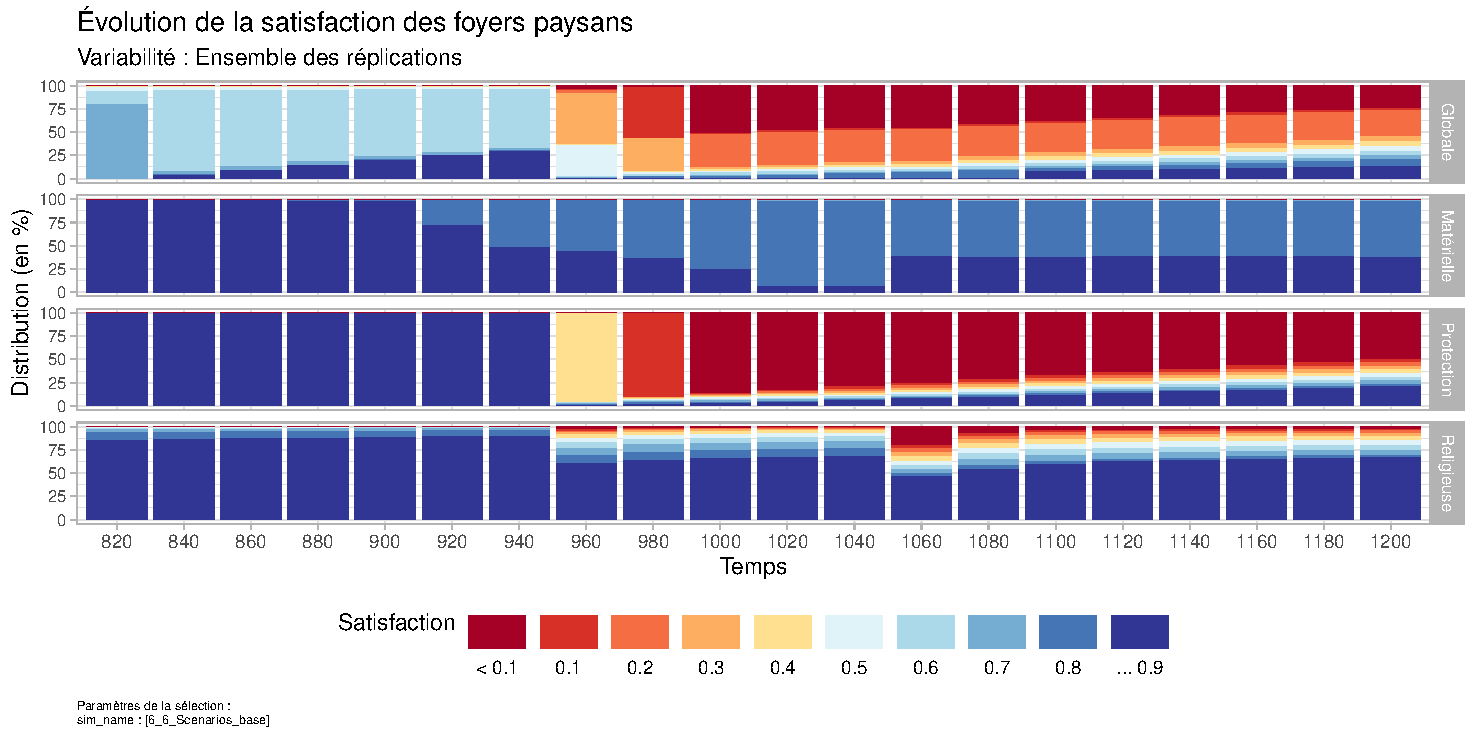
\includegraphics[width=\linewidth]{img/results_6_6/FP_Satisfaction_Haut.pdf}
	\caption{Satisfaction des foyers paysans.}
	\label{fig:results-fp-satisfaction}
\end{figure}

La lecture de la \cref{fig:results-fp-satisfaction}, qui présente les types de satisfaction des foyers paysans au cours de la simulation, vient appuyer cette analyse.
On y retrouve les trois phases observées dans les sorties de simulation.
Avant 960, la satisfaction augmente, et les migrations diminuent avec elle.
En 960, c'est bien la satisfaction de protection qui diminue fortement, poussant les foyers paysans à migrer et déclenchant la seconde phase migratoire.
En 1060, on retrouve le même effet, de moindre ampleur cependant, dans la satisfaction religieuse. À nouveau, les satisfactions diminuent et une nouvelle phase migratoire est initiée.
\clearpage

\begin{figure}[H]
	\centering
	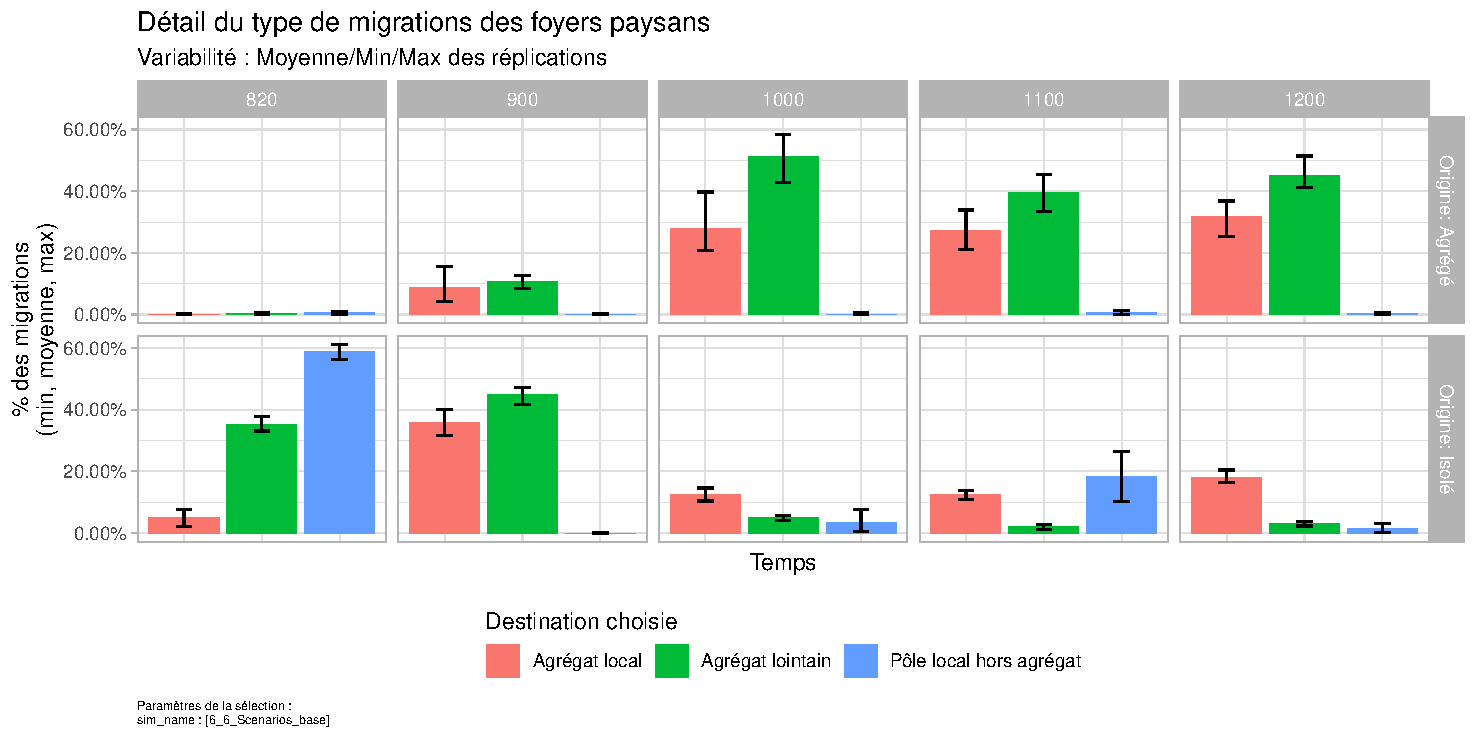
\includegraphics[width=\linewidth]{img/results_6_6/FP_DeplacementsDetail_Haut.pdf}
	\caption{Types de migration des foyers paysans.}
	\label{fig:results-fp-migrations-detail}
\end{figure}

En observant le détail des migrations (\cref{fig:results-fp-migrations-detail}), non continu dans le temps contrairement aux graphiques précédents, on ne retrouve que deux périodes.
La figure nous renseigne toutefois sur une autre dimension liée aux migrations, en fonction ici de l'origine et de la destination des foyers paysans.
On peut alors préciser les observations précédentes : quels foyers paysans migrent, et où ?

En 820 et en 900, la plupart des migrations proviennent de foyers paysans isolés.
Ces migrations, locales et lointaines, permettent aux foyers paysans de rejoindre un agrégat, quel qu'en soit la place dans la hiérarchie.
En 1000 et après, les foyers paysans isolés représentent encore une part substantielle de la population (50\% d'après la \cref{fig:results-concentration-fp}), mais leur poids relatif dans les migrations est devenu bien plus faible que celui des migrations entre agrégats de population.
Après une première période de concentration arrive une période de choix hiérarchique pour les foyers paysans, où les différences d'attractivité des agrégats jouent alors un rôle prépondérant.
Cela indique aussi qu'à partir de cette période, les agrégats sont pour la plupart pérennes et se livrent alors une compétition.

\paragraph{Dissémination du peuplement.}

Dans le modèle, la répartition des paroisses constitue un observable intéressant pour évaluer la dissémination du peuplement.
Comme les paroisses ont vocation à desservir la population des foyers paysans, elles constituent un proxy de sa répartition tout au long du temps.
Les indicateurs liés (\cref{fig:results-paroisses-nb,subfig:results-paroisses-carte,subfig:results-paroisses-superficie}) donnent une lecture satisfaisante du processus de dissémination.

En premier lieu, on note que le nombre d'églises paroissiales augmente de manière régulière au cours du temps, avec un saut entre 1060 et 1080, comme pour de nombreux indicateurs vu auparavant (\cref{fig:results-paroisses-nb}).
Par rapport aux logiques de création et de promotion, on remarque que le nombre d'églises non paroissiales chute fortement à la même période.
Ces églises se voient attribuer les droits paroissiaux, et on peut dès lors affirmer que l'augmentation du nombre de paroisses de 1080 correspond surtout à des églises rurales puisque ce sont elles qui sont susceptibles d'être promues par le mécanisme (voir \cref{sssec:paroisses}).
\clearpage

\begin{figure}[H]
	\centering
	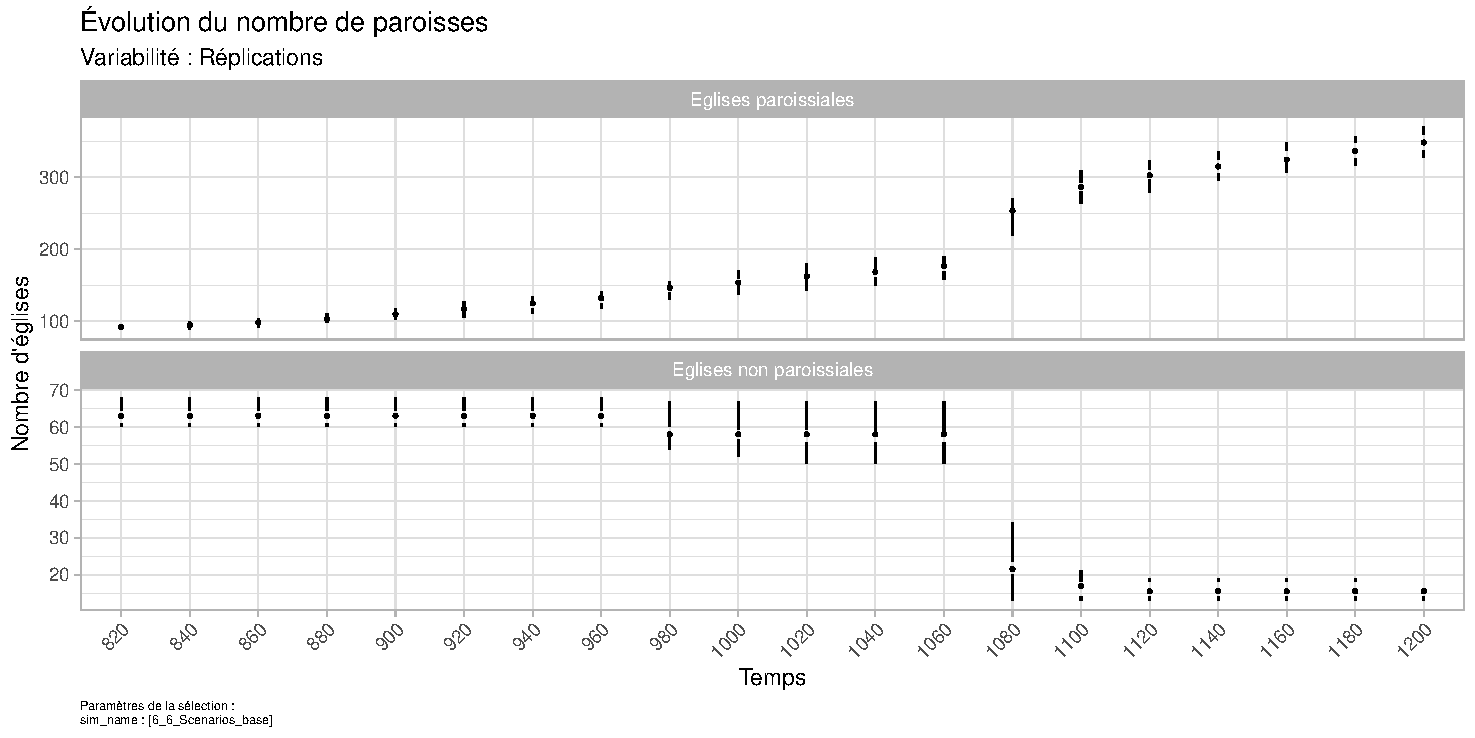
\includegraphics[width=\linewidth]{img/results_6_6/Paroisses_Nb_Haut.pdf}
	\caption{Nombre de paroisses.}
	\label{fig:results-paroisses-nb}
\end{figure}

On constate nettement dans la \cref{subfig:results-paroisses-carte} une densification généralisée du maillage paroissial.
Cette densification est visible à deux niveaux.
En premier lieu, le maillage est de plus en plus dense globalement : la superficie moyenne des paroisses diminue (visible aussi dans la \cref{subfig:results-paroisses-superficie}), et visuellement, on constate une certaine homogénéisation et normalisation des paroisses.
Les très grandes paroisses initiales (plus de 50 km² dans la \cref{subfig:results-paroisses-superficie}), surtout situées dans les marges de la région, disparaissent progressivement à mesure qu'elles sont subdivisées par le mécanisme de création/promotion d'églises paroissiales rurales (\cref{meca-paroisses}).

\begin{figure}[H]
	\centering
	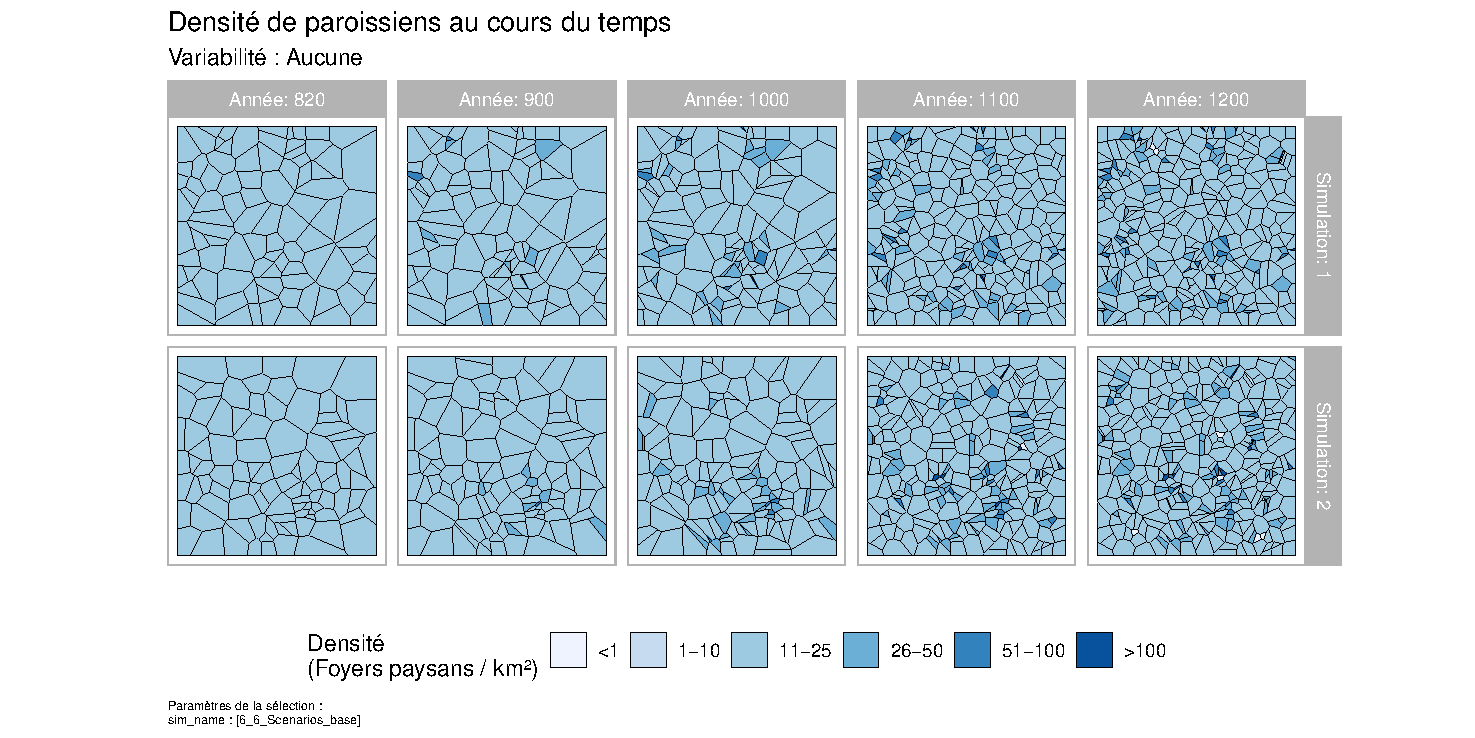
\includegraphics[width=\linewidth]{img/results_6_6/Paroisses_Carte_Haut.pdf}
	\caption{Densité des paroisses et des paroissiens.}
	\label{subfig:results-paroisses-carte}
\end{figure}
\clearpage

\begin{figure}[H]
	\centering
	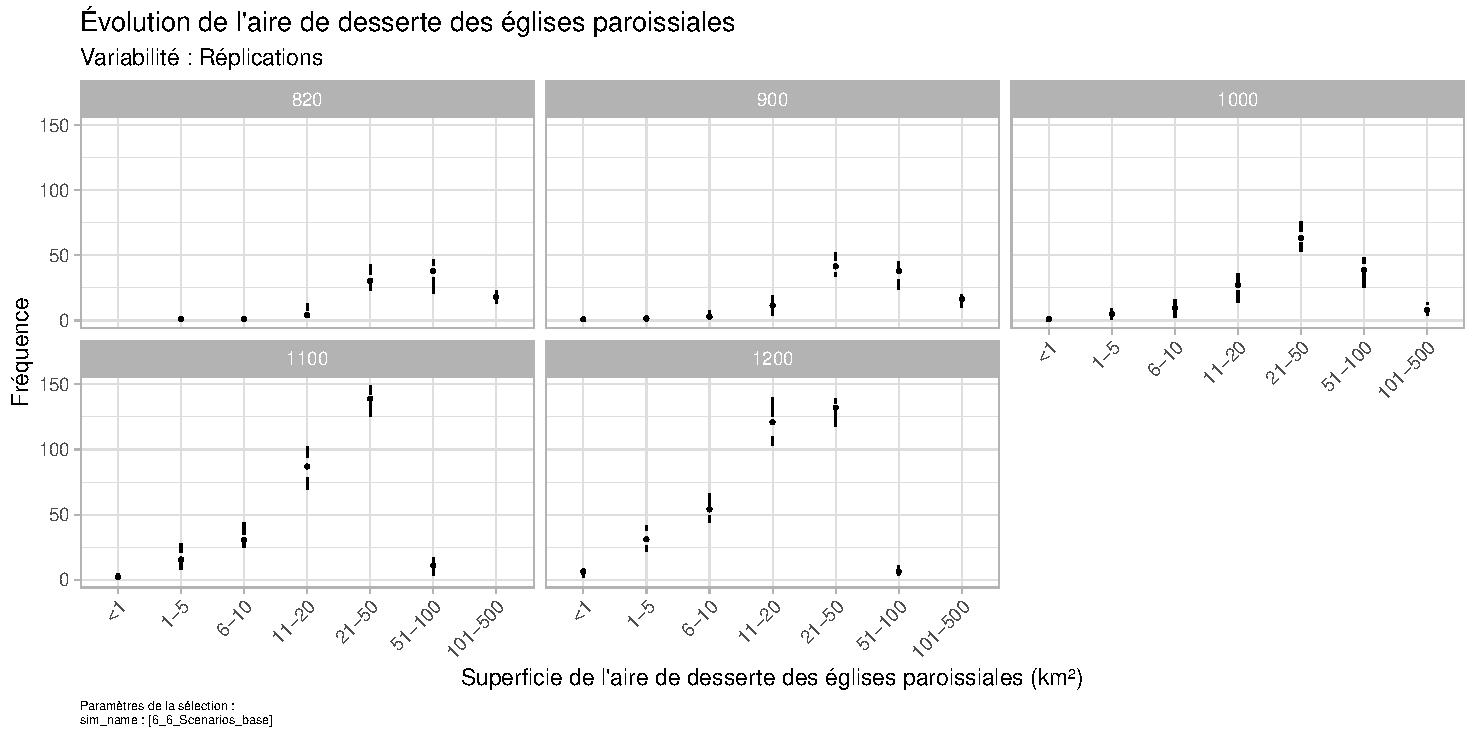
\includegraphics[width=\linewidth]{img/results_6_6/Paroisses_Superficie_Haut.pdf}
	\caption{Superficie des paroisses.}
	\label{subfig:results-paroisses-superficie}
\end{figure}

En second lieu, à l'échelle infra-régionale, on note une intensification très locale de paroisses (le maillage se densifie fortement), dans lesquelles les densités de foyers paysans sont importantes.
Ces densifications locales sont représentatives des agrégats les plus importants, qui peuvent comporter jusqu'à près d'une dizaine d'églises paroissiales\footnote{
	On peut le constater dans la \cref{fig:results-nb-poles-agregats}-a, où les pôles les plus importants de la hiérarchie contiennent une douzaine d'attracteurs. Si l'on considère que ces pôles contiennent un agrégat et un château, on peut en déduire qu'il y a aussi une dizaine d'églises paroissiales au service de cet agrégat.
}.

Ces deux niveaux d'observation, combinés à la cartographie des agrégats (\cref{fig:results-carte-agregats_poles}), montrent que le modèle produit bien une dispersion du peuplement dans l'espace : on voit des concentrations locales, mais à l'échelle globale, les mailles sont harmonisées par le bas, signe que des petits agrégats apparaissent dans l'ensemble du monde simulé.

\begin{figure}[H]
	\centering
	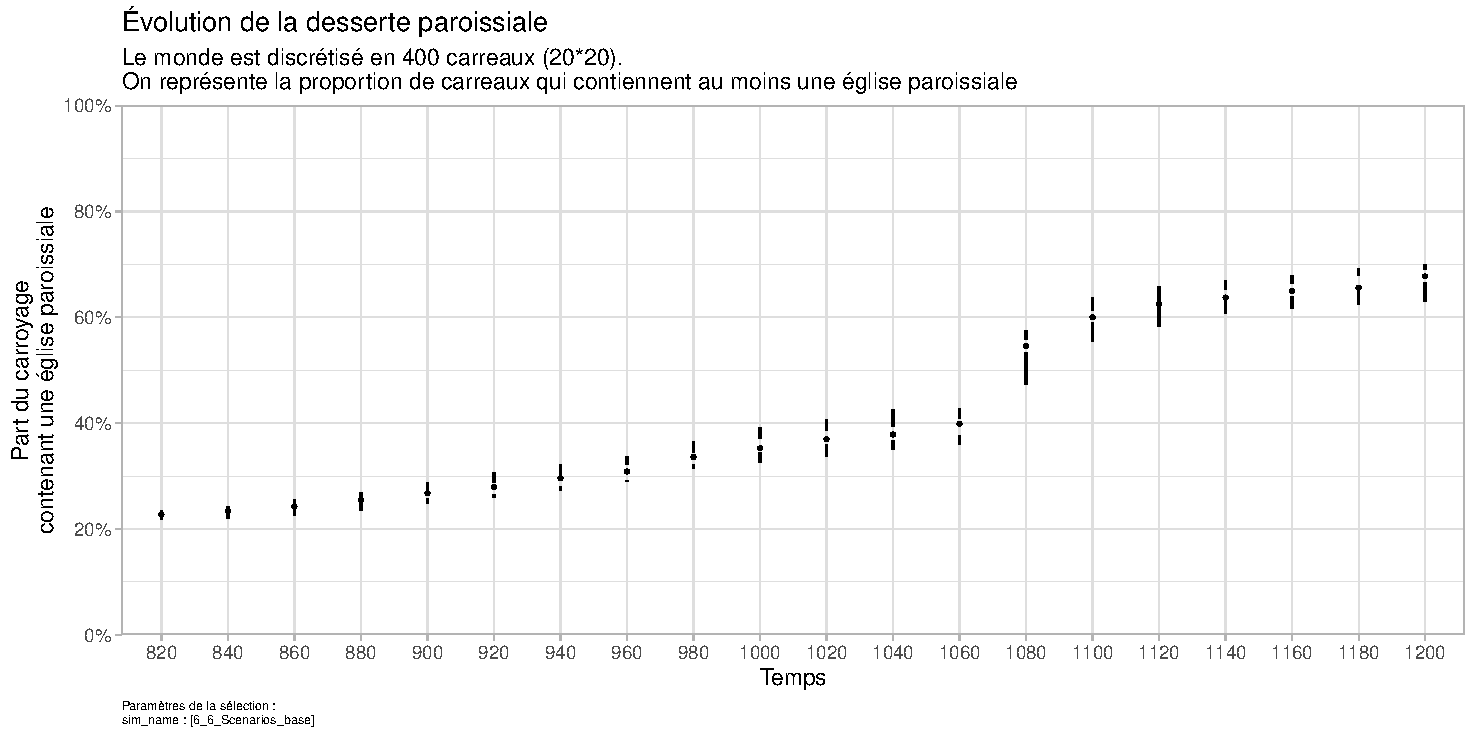
\includegraphics[width=\linewidth]{img/results_6_6/Paroisses_Desserte_Haut.pdf}
	\caption{Couverture de la desserte paroissiale.}
	\label{fig:results-paroisses-desserte}
\end{figure}

Pour préciser cette mesure et obtenir un indicateur spatial agrégé des réplications\footnote{
	Au contraire des cartes, qui ne peuvent décrire que des simulations particulières, l'agrégation spatiale n'étant pas possible dans le monde théorique fluctuant qui est simulé (voir le \cref{chap:chap6}, \cref{subsec:genericite-donnees-simul} pour plus de précision).
}, on peut quantifier la couverture de l'espace qu'occupent les églises paroissiales.
Dans la \cref{fig:results-paroisses-desserte}, le monde simulé est discrétisé en 400 carreaux de 4 km de côté et on procède à un comptage de la proportion de ces carreaux qui contiennent au moins une église paroissiale à chaque date.
La lecture de la figure montre que la part du monde qui est située à proximité d'une église paroissiale augmente au cours du temps, avec un rythme comparable à celui de l'augmentation du nombre d'églises paroissiales (\cref{fig:results-paroisses-nb}).
Cela constitue un indice qui peut laisser penser que l'augmentation du nombre de paroisses dans le modèle est bien un phénomène qui est réparti de manière homogène dans l'espace.
\simfeodal{} est donc bien en capacité de reproduire les processus de fixation et de dissémination qui ont été observés empiriquement en Touraine et plus généralement dans l'Europe du Nord-Ouest.



\bigskip
\paragraph[Conclusion intermédiaire]{}
De manière générale, \simfeodal{} parvient ici entièrement à reproduire le double fait stylisé recherché : fixation et dissémination du peuplement.
Pourtant, plus encore que pour les dimensions précédentes, il nous paraît extrêmement difficile d'aller plus loin dans le calibrage du modèle.
La raison en est principalement la difficulté de l'évaluation quantitative de ces phénomènes.
Parmi les indicateurs de sortie de simulation étudiés, ceux correspondant à cette dimension d'analyse sont les plus intrinsèquement spatio-temporels, et se prêtent donc mal à des agrégations synthétiques.
Certes, le champ de l'analyse spatiale s'est en partie constitué pour répondre à ce type de problème, en trouvant des mesures synthétiques et variées permettant de décrire et de comparer des semis de points, correspondent-ils à des entités ou à des époques différentes.

Pourtant, et on y reviendra plus extensivement dans le chapitre suivant, on constate ici une limite de notre méthode d'évaluation des simulations, au vu des données et connaissances empiriques dont on dispose.
Un espace théorique, simulé et très variable localement comme celui de \simfeodal{} se prête en effet mal à une agrégation de données.
Les différentes réplications d'un modèle ne partagent ainsi pas véritablement de référentiel spatial commun en dehors des limites du monde simulé : les positions des agrégats, des églises, des paroisses, sont en effet incomparables d'une réplication à l'autre.
De manière générale, les configurations spatiales générées par le modèle -- les semis de ces agents -- sont donc non agrégables et donc difficilement comparables entre les expériences autrement que d'une manière visuelle.
Sans données empiriques susceptibles de préciser les taux d'occupation attendus, les mesures de dispersion des semis d'églises, de villages, etc., on ne peut pousser l'évaluation visuelle plus avant.
L'usage de mesures synthétiques, tirées de l'analyse spatiale, pour décrire ces configurations spatiales serait de plus peu adapté puisque ne reposant pas sur des sources empiriques suffisamment précises.
\clearpage
%Pour pousser l'évaluation et être en mesure de comparer de nouvelles simulations par le biais des indicateurs présentés ici, au moins pour ceux relatifs à la fixation et dissémination, il faudrait sans doute mener des études de cas plus approfondies sur les sorties du modèle.
%On pourrait par exemple suivre des ensembles de foyers paysans ou d'agrégats tout au long des simulations pour analyser plus finement leur comportement.
%Mais même alors, le manque de sources empiriques se ferait forcément et fortement ressentir : on pourrait peut-être isoler la différence entre des simulations, mais serait-il vraiment possible de les départager ?


\subsection{Après le calibrage, comment affiner le modèle ? \label{subsec:depasser-calibrage}}

Dans l'ensemble, l'analyse des résultats montre que cette version calibrée de \simfeodal{} répond aux attentes en matière de reproduction des faits stylisés identifiés d'après les connaissances expertes.
Le modèle aboutit bien sur une polarisation de l'habitat, autour de pôles d'attractions très hiérarchisés et disséminés dans l'espace simulé.
Cette polarisation débouche sur une structure spatiale pérenne, due à la fixation des foyers paysans au sein d'agrégats qui composent le système de peuplement.

Le modèle \simfeodal{} est donc satisfaisant vis-à-vis de ce pour quoi il a été conçu, développé et calibré.
En comparant les dizaines de versions successives du modèle, ce constat s'affirme avec plus de force : chaque version a permis des améliorations notables, depuis une version 0 qui parvenait tout juste à une concentration du peuplement jusqu'aux versions plus récentes, préalables à la version 6.6 ici présentée, chacune ayant renforcé, sur des points spécifiques, l'ajustement aux connaissances expertes.
Certains indicateurs (par exemple ceux liés aux églises), toutefois, et en particulier les indicateurs quantitatifs qui donnent un aperçu global et synthétique des résultats du modèle (\cref{ssec:results-global}), demeurent assez éloignés des objectifs fixés.
Il serait donc envisageable de chercher à prolonger et affiner le calibrage du modèle afin que sa capacité à reproduire les faits stylisés soit améliorée.

Il nous semble toutefois que cette démarche ne vaudrait pas le temps et l'effort qu'elle appelle.
Ce sentiment s'appuie sur deux raisons distinctes : la première liée au domaine empirique et la seconde au domaine du modèle.

\paragraph{Calibrer sans sur-ajuster.}
Dès le calibrage des paramètres d'\textit{input} (\cref{sssec:calibrage-inputs}), on mentionnait les difficultés du recueil de sources empiriques -- matérielles ou littéraires -- pour des éléments qui paraîtraient pourtant triviaux et indispensables à tout géographe contemporain.
La population de la région et son évolution sur la période considérée, par exemple, ne peut donner lieu qu'à une estimation très grossière.
De plus, on ne peut avoir aucune garantie, ni même d'espoir, que de futures sources permettent de mieux les spécifier.

Dans le même temps, on cherche à améliorer l'ajustement des sorties du modèle à des objectifs fixés sur ces sources empiriques floues et lacunaires.
L'expertise des thématiciens du groupe de modélisation de \simfeodal{} a permis de définir ces objectifs, mais ceux-ci présentent un niveau de précision parfois assez faible.
Par exemple, on cherche à ce que \simfeodal{} puisse atteindre 20\% de foyers paysans isolés en fin de simulation.
Les versions successives du modèle ont permis de faire descendre ce taux d'environ 60\% à environ 20\%.
En considérant que les connaissances empiriques donnent une estimation plausible située entre 20\% et 30\%, quel sens y aurait-il à départager des modèles selon qu'ils atteignent 25\% ou 27\% ?

Ce problème, qui se pose pour chacun des objectifs et attendus du modèle, est un cas typique de sur-ajustement, ou \og overfitting\fg{}.
Sur le plan thématique, chercher à coller absolument à un objectif sans tenir compte du degré d'incertitude de ce dernier, bien plus élevé que celui que le modèle est en mesure de produire, n'a ainsi aucun sens.
Sur le plan méthodologique, on peut aussi noter qu'à mesure que le calibrage du modèle progresse, les \og gains\fg{} de chaque étape se font plus faibles.
Chercher à améliorer le calibrage du modèle reviendrait alors à différencier des modèles sur des critères de plus en plus précis, alors même que le niveau de précision de ces critères est en lui-même statique et d'un ordre de grandeur inférieur.

Sans connaissances empiriques supplémentaires, il n'est pas possible de véritablement mieux calibrer \simfeodal{}, qui a déjà atteint un niveau de détail qui dépasse presque celui des connaissances expertes par le prisme desquelles tout résultat doit être étudié pour porter un sens.


\paragraph{Calibrer un modèle (très) complexe.}
Un autre élément concourt aussi à la difficulté d'améliorer le modèle, cette fois-ci directement lié aux choix de conception de \simfeodal{}.
Comme décrit dans les deux premiers chapitres, \simfeodal{} est un modèle exploratoire, plus descriptif (KIDS) que parcimonieux.
Les paramètres y sont très nombreux, de même que les mécanismes qu'ils ajustent.
Les agents du modèle interagissent, et, avec eux, les mécanismes qui les caractérisent s'entrecroisent et s'imbriquent.
Si l'on a une connaissance parfaite de chaque mécanisme (puisqu'on les a conçus et implémentés), il est difficile d'avoir une connaissance de même ordre sur l'aboutissement de leurs interactions, c'est la raison d'être de la simulation.

Dans des modèles moins descriptifs, mêmes complexes, on peut avoir des idées relativement précises de la combinaison des mécanismes, et donc une bonne intuition des sorties de simulation qui en résulteront.
Dans un modèle comme \simfeodal{}, les paramètres sont trop nombreux pour que ce soit réellement possible, et les résultats contre-intuitifs ont été fréquents dans les différentes étapes de paramétrage et de calibrage du modèle.
Ces éléments contre-intuitifs, surprenants, sont extrêmement stimulants du point de vue de la connaissance des effets du modèles.
Ils placent les modélisateurs et évaluateurs dans une démarche abductive où l'identification de l'explication des diverses surprises permet de mieux comprendre le fonctionnement effectif du modèle et, à partir de là, du système modélisé (voir \cref{subsec:construction-connaissance-explo}).

Dans la recherche d'un calibrage mieux adapté, cette approche abductive ne permet toutefois pas véritablement de progresser ailleurs que dans la connaissance du modèle en lui-même.
À mesure que le calibrage se précise, la complexité du modèle apparaît renforcée.
Comme dans le principe des vases communicants, une modification de valeur d'un paramètre est presque systématiquement assortie d'une réaction imprévu (et imprévisible) sur un indicateur différent de celui sur lequel le paramètre devait agir.
Chaque modification de paramètre devrait donc donner lieu à de nouveaux ajustements d'autres paramètres, jusqu'à obtenir, dans le meilleur des cas, un ensemble de valeurs de paramètres stable.

Pour améliorer le calibrage, et éviter ces allers-retours imprévisibles entre paramètres, il manque alors une vision plus globale des réactions engendrées par les modifications de chaque paramètre.
Une telle vision permettrait de ré-organiser les paramètres, pour chaque indicateur de sortie, en ensembles thématiques dont l'on ferait systématiquement co-varier les valeurs testées afin d'approcher de l'objectif de manière harmonisée.
Pour mieux comprendre les aboutissements du modèle, il est dès lors nécessaire de l'explorer de manière plus systématique, en essayant de comprendre l'influence réelle de chacun des paramètres plutôt que de tâtonner, de manière experte certes, en agissant sur les paramètres qui nous semblent intuitivement les plus importants.
%Une telle exploration, plus systématique, de grande ampleur et cherchant à dépasser l'intuition, ne peut se mener que sur une quantité réduite d'éléments du modèle (indicateurs de sortie, mais aussi intervalle de validité des paramètres), et cela requiert dès lors de réussir à synthétiser de manière manifeste, quantifiée, les attentes que l'on a vis-à-vis des résultats du modèle.
Ce sont ces objectifs de compréhension plus fine du comportement du modèle que nous allons poursuivre dans la suite de ce chapitre, au moyen d'analyses de sensibilité.


\clearpage
\section{Analyser la sensibilité de SimFeodal \label{sec:ana-sensib}}

Parmi les nombreuses méthodes dédiées à l'évaluation de modèles, il en est une que l'on retrouve dans tous les manuels et dans la plupart des articles dédiés à la présentation de modèles.
Il s'agit de l'analyse de sensibilité, catégorie en fait plurielle qui regroupe l'ensemble des méthodes vouées à tester ou à explorer la stabilité d'un modèle face aux éléments qui le composent :
poids des \textit{inputs} dans les résultats obtenus ; variabilité des résultats selon les valeurs de paramètre choisies ; variabilité des résultats due à l'aléa etc.
Ces méthodes sont extrêmement nombreuses et constituent presque un champ scientifique à part entière, lié à l'évaluation de modèles à base d'agents ou statistiques.

Parmi celles-ci, les méthodes les plus classiques \autocite[257]{crooks_agent-based_2019} visent à \og déterminer l'influence des paramètres sur les sorties du modèle.\fg{} \autocite[75]{ginot2005explorer}.
Il s'agit de faire varier les valeurs des paramètres et de mesurer les écarts produits dans les sorties.
Le plus souvent, cette mesure est quantitative, par exemple sous la forme d'un \og indice de sensibilité\fg{} qui dépend des variations des sorties mais aussi de l'amplitude de la variation des paramètres\footnote{
	Cette prise en compte de la variation des valeurs de paramètre, par exemple dans l'indice proposé par \textcite[258]{crooks_agent-based_2019} et dérivé de celui de \textcite{hamby_review_1994} (in \cite[201]{osullivan_spatial_2013}), permet de s'assurer, lors de la comparaison de la sensibilité des paramètres, que les valeurs comparées sont bien comparables.
	Pour prendre l'exemple du modèle de Schelling, il s'agit de s'assurer qu'on ne compare pas une variation de 0,1\% du seuil de tolérance avec une variation de 20\% dans la part d'espace vide.
	Dans ces indices, les amplitudes des valeurs testées sont en fait normalisées.
}.

Les analyses peuvent être menées paramètre par paramètre, en conservant par exemple des valeurs fixes pour un jeu de paramètres de base (issus de calibrage par exemple) et en faisant varier un unique paramètre à la fois (analyse de type \textit{OFAT}, \og \textit{one factor at a time}\fg{}).
On peut aussi procéder de manière combinatoire, en croisant des valeurs pour tous les paramètres, c'est-à-dire en analysant la sensibilité du modèle aux interactions entre paramètres.

Les analyses de sensibilités sont souvent présentées comme une pratique indispensable à la validation de modèle : on les retrouve dans l'ensemble des schémas relatifs à la démarche d'évaluation du \cref{chap:chap3} (\cref{fig:schema_kluegl,fig:schema_ngo}).
Au-delà de la validation des modèles, ce type d'analyse constitue un outil incontournable pour aider à la compréhension d'un modèle, sans nécessairement chercher à en éprouver la validité.
En effet, cette méthode repose sur l'exploration d'un modèle par le prisme de ses réactions face aux paramètres choisis, et permet ainsi de mener une étude approfondie de l'influence des paramètres.
Dans certains modèles, une analyse de ce type a par exemple permis de rendre plus parcimonieux un modèle KISS, en mettant en lumière le peu d'influence d'un paramètre sur l'ensemble des sorties d'un modèle.
C'est le cas dans le travail de thèse de \citeauteur{schmitt_modelisation_2014}, où une analyse de sensibilité a révélé la relative inutilité de l'un des 6 paramètres mobilisés dans le modèle SimpopLocal \autocite[224-225]{schmitt_modelisation_2014}.

Dans le cadre d'un modèle exploratoire, où les très nombreux paramètres comportent vraisemblablement une part de redondance, l'ambition n'est pas de rechercher à réduire la masse de paramètres à tout prix, mais plutôt d'aider à comprendre lesquels ont la plus grande influence sur le modèle.
Ainsi, pour \simfeodal{}, l'analyse de sensibilité doit permettre de gagner en compréhension du modèle, et en conséquence, des dynamiques modélisées.


%De manière plus générale, une analyse de sensibilité quantitative requiert à minima des objectifs quantitatifs synthétiques, hiérarchisés et parcimonieux, ce qui n'est pas la démarche empruntée dans \simfeodal{}.
Dans cette partie, nous nous en tiendrons à une analyse de sensibilité sommaire, orientée vers une évaluation visuelle, à l'instar des autres démarches d'évaluation du modèle mises en places.
La nature descriptive et exploratoire -- donc avec un modèle dont les composants, dont les paramètres, sont hétérogènes -- de \simfeodal{} rend en effet l'application des méthodes classiques de l'analyse de sensibilité assez difficile : les paramètres ne sont pas tous quantitatifs, certains fonctionnent par paires, par grappes etc.
%Dans cette partie, nous nous en tiendrons à une analyse de sensibilité grossière, orientée vers une évaluation visuelle, à l'instar des autres démarches d'évaluation du modèle mises en places.
L'évaluation visuelle nous semble alors tout à fait adaptée à cette hétérogénéité de paramètres, et à ce titre, nous nous inscrivons pleinement dans le raisonnement de \citeauteur{hirtzel2015exploration}, d'autant plus que ce raisonnement est tenu dans une thèse dont l'analyse de sensibilité de modèles descriptifs est un enjeu principal :
\begin{quotation}
	\og Ces différents constats nous ont conduit à procéder à des analyses de sensibilité locales, avec la méthode OAT\footnote{
		[C'est un autre acronyme de \og \textit{one factor at a time}\fg{}, identique à \textit{OFAT} que nous utilisons dans cette partie.]
	}, en modifiant les valeurs de chacun des paramètres les unes après les autres, toutes choses égales par ailleurs, c’est-à-dire tous les autres paramètres étant fixés à leur valeur par défaut \textelp{}.
	Ce choix n’est pas unique dans la modélisation individu-centrée : la méthode OAT est utilisée dans plusieurs travaux en géographie ou en écologie (Ginot et al., 2006; Sanders et al., 2006; Laperrière et al., 2009; Schouten et al., 2014).
	
	Nous n’avons pas jugé indispensable le calcul d’indices de sensibilité pour étudier la sensibilité des résultats de simulation aux différents paramètres du modèle.
	Une analyse graphique à la manière de Sanders et al. (2006\st{a}), Laperrière et al. (2009) ou encore Schouten et al. (2014) nous a paru suffisante, dans un premier temps.
	Ainsi, pour reprendre les termes évoqués dans les deux sous-parties précédentes, l’analyse de sensibilité présentée dans ce chapitre est une analyse locale (OAT), avec des évaluations qualitatives de l’impact de l’incertitude émanant des valeurs de paramètres sur différents résultats de simulation.\fg{}\\
	\mbox{}~ \hfill \cite[251-252]{hirtzel2015exploration}
\end{quotation}


\subsection{Méthodologie - Analyse visuelle de sensibilité.}

Dans cette partie, nous décrivons et justifions brièvement la méthodologie mise en place pour l'analyse de sensibilité de \simfeodal{}.
Les sources informatiques, précises, de la démarche sont disponibles dans le dépôt du modèle\footnote{
Dans la branche \og SensibilityAnalysis\fg{} :\\ \href{https://github.com/SimFeodal/SimFeodal/blob/SensibilityAnalysis/models/AnaSensib_6_5.gaml}{https://github.com/SimFeodal/SimFeodal/tree/SensibilityAnalysis/models}
}.
Le détail des paramètres, les outputs du modèle, les traitements et les sorties graphiques sont disponibles quant à eux à cette adresse :\\ \href{https://github.com/RCura/these/tree/master/chap5/src/AnalyseSensibilite}{https://github.com/RCura/these/tree/master/chap5/src/AnalyseSensibilite}

\subsubsection{Calcul de la sensibilité.}

Nous avons choisi de mener l'analyse de sensibilité de \simfeodal{} en empruntant l'approche \textit{OFAT}, c'est-à-dire en faisant varier les paramètres un par un.
Il convient en effet de rappeler que ce modèle est caractérisé par un nombre important de paramètres : près de 70.
En ne choisissant que 5 valeurs pour chaque paramètre et pour croiser tous les paramètres, une analyse de type plan factoriel demanderait l'exécution de $5^{70} \times 20_{\text{[replications]}}$, soit environ $10^{50}$ simulations\ldots{}
%Dans un modèle complexe où les agents sont en interactions les uns avec les autres, cette approche est forcément biaisée et lacunaire au regard d'approches plus avancées comme les méthodes d'exploration de l'espace des paramètres.
Une approche plus simple, de type OFAT, nous paraît dès lors la seule à être applicable dans le cas de \simfeodal{}.


\paragraph{Paramètres.}
Dans une analyse de sensibilité, le premier choix à faire concerne les paramètres à analyser.
Dans les modèles statistiques ou KISS, l'analyse de chacun des paramètres est une évidence.
Dans des modèles plus descriptifs tels que \simfeodal{} (ou les modèles analysés par \textcite{hirtzel2015exploration}), on procède souvent à une sélection des paramètres afin de réduire l'ampleur de la tâche.
Par exemple, quand certains paramètres ont un ancrage empirique fort, on peut considérer qu'ils se comportent davantage comme des constantes que comme des paramètres, qu'ils n'auront jamais à varier, et ne requièrent ainsi pas d'être analysés.

Dans \simfeodal{}, on aurait pu par exemple écarter l'analyse des paramètres de contexte les plus inscrits dans les connaissances empiriques.
Pourtant, comme nous envisageons d'éprouver le modèle sur des scénarios susceptibles de faire varier tous les types de paramètres -- par exemple portant sur des régions et des périodes différentes -- il nous a semblé important de tester aussi ces paramètres.
On a donc opté pour une analyse de sensibilité de l'ensemble des paramètres du modèle.
\simfeodal{} comporte dans les faits 70 paramètres, mais en pratique, certains n'ont aucun sens quand ils sont mobilisés seuls.
Par exemple, deux paramètres définissent le rayon minimum et maximum des zones de prélèvement.
Il n'y a pas grand interêt à faire varier l'un sans l'autre.
Dans l'analyse de sensibilité, nous considérons ces deux paramètres comme un unique paramètre à analyser, qui ne prend pas la forme d'une valeur numérique simple, mais plutôt celle d'une étendue.

Pour cette analyse de sensibilité, nous avons au final analysé 57 \og paramètres\fg{}, certains de forme numérique simple, d'autres sous formes d'étendues, et enfin quelques-uns ayant des structures plus complexes (étendues changeant au cours du temps par exemple).

\paragraph{Méthode.}
La méthode choisie est simple : on définit un jeu de paramètres de base, issu du calibrage, et pour chacun des paramètres, on exécute un ensemble de simulations en faisant varier ce paramètre autour de sa valeur de base.
Comme pour toute simulation d'un modèle stochastique, il est indispensable de procéder à des réplications de ces simulations.

Comme le nombre de paramètres était déjà important, que le nombre de réplications (20) l'était lui aussi, on a choisi de mener une analyse de sensibilité assez réduite, en ne testant, pour chaque paramètre, que 5 valeurs différentes.
Ce nombre amène déjà à l'exécution de $57_{\text{[paramètres]}} \times 5_{\text{[valeurs]}} \times 20_{\text{[réplications]}} = 5700$ simulations, ce qui est une quantité importante de simulations au regard de toutes celles qui ont été menées dans les étapes de paramétrage et d'évaluation visuelle du modèle.

\paragraph{Étendue.}\label{par:etendue-parametres}
Dans une analyse de sensibilité classique, on cherche à tester des variations de paramètres comparables, c'est-à-dire centrées autour des valeurs par défaut et présentant des variations relatives de même ampleur.
Par exemple, pour un modèle dont le premier paramètre vaut 10 et le second 100, on cherchera à répartir les valeurs testées de manière comparable : 
le premier paramètre sera testé aux valeurs [0, 5, 10, 15 et 20], et le second pour [0, 50, 100, 150 et 200].

Dans un cas réel, cette règle est difficile à suivre : on a ici pris l'exemple de paramètres quantitatifs \og de stock\fg{}, qui ne sont comparables qu'entre eux.
Dans \simfeodal{}, certains paramètres ont des structures bien plus difficilement comparables, à l'instar des étendues.
Comment rendre comparable cinq variations autour d'un stock de 10, et cinq variations autour d'une étendue de 1500 m à 5000 m ?
L'étendue des possibles transformations pour ces étendues est bien plus important : diminution, augmentation, translation, etc.
Contrairement aux variables de stocks qui ne comportent qu'une dimension, les étendues sont en effet composées de deux dimensions, et la quantité de variation possibles suit donc une loi de puissance.

Ce problème se pose avec plus de force pour les paramètres qui évoluent en fonction du temps.
Par exemple, le paramètre qui agit sur la satisfaction protection des foyers paysans, a une valeur composite (de type \textit{map}, voir \cref{lst:maps-gama} dans le \cref{chap:chap2}) qui vaut \og $0$ entre 800 et 940; $0.2$ en 960 ; $0.4$ en 980 ; $0.6$ en 1000 ; $0.8$ en 1020 ; et $1$ à partir de 1040\fg{}.
C'est donc un paramètre à trois dimensions : une valeur (dimension 1) qui évolue selon des intervalles de temps (dimensions 2 et 3)\footnote{
	Ces dimensions sont en fait moins \og complètes\fg{} que la première, étant donné que les bornes temporelles ont une contrainte de continuité.
}.
Pour l'analyser dans son entièreté, il faudrait supprimer la variation en testant plusieurs valeurs, mais aussi changer le rythme de cette variation, en décaler l'étendue temporelle, en changer l'intensité etc.
Sous bien des aspects, ce paramètre peut être considéré comme qualitatif, et les variations qu'on lui appliquera dans l'analyse de sensibilité ne peuvent être que très subjectives et intrinsèquement différentes.

Face à ces difficultés, nous avons adopté une position générale acceptant la subjectivité, la non-comparabilité, mais cherchant à explorer des valeurs \og caractéristiques\fg{} pour ce type de paramètres : activation et désactivation du mécanisme associé, valeur de base, et augmentation et diminution de l'ampleur de la valeur de paramètre.
Dans l'ensemble, les valeurs de paramètres choisies (disponibles dans l'\cref{annexe:A}, \cref{annexe:A3}) ne sont que peu comparables de manière numérique, mais elles apportent un éclairage précieux sur le comportement du modèle en fonction de ses paramètres.

\paragraph{\textit{Outputs}.}
Le \cref{chap:chap4} donnait des ordres de grandeur de la masse des données produites par le modèle, autour de 10 Mo pour une simulation.
Avec 5700 simulations, un enregistrement complet des données aurait représenté plus de 50 Go de données et plus de 50 milliards de lignes de données à pré-traiter, intégrer et analyser dans la base de données.

Cette masse de données pose des problèmes techniques tant que méthodologiques.
Sur le plan technique, les solutions de stockage et d'interrogation de données utilisées pour l'exploration des données ne sont pas adaptées à une telle masse, du moins sans avoir recours à des infrastructures physiques coûteuses (serveurs équipés de cartes graphiques extrêmement puissantes etc.).
En termes de capacité d'archivage, il est donc obligatoire de réduire considérablement la masse des données.

Sur le plan méthodologique, l'exploration visuelle de milliers de simulations organisées selon les variations des valeurs d'une soixantaine de paramètres nous semble répondre à des caractéristiques très particulières.
Les méthodes et outils d'exploration interactive mis en place jusque là (\cref{sec:SimEDB}) ne sont pas adaptés à ce type d'usages.
%Pour une analyse qui n'est pas au cœur de notre démarche de co-construction, cela représentait un poids bien trop important.
Nous avons donc choisi, par soucis de lisibilité, de réduire autant que possible la production d'indicateurs de sorties de simulations pour cette analyse de sensibilité.

%D'abord, nous n'enregistrons l'état du modèle qu'à son pas de temps final (en 1200) plutôt que tout au long de son déroulement.
D'abord, nous n'enregistrons que l'état final du modèle et non pas l'ensemble des états intermédiaires.
Il n'est ainsi pas véritablement gênant de perdre l'aspect dynamique et la possibilité de comparer les rythmes du changement entre les simulations.
En effet, l'analyse de sensibilité doit se concentrer sur aussi peu d'objectifs que possible.
Pour les mêmes raisons, on a décidé de n'extraire que des données très agrégées du modèle.
L'analyse de sensibilité s'appuie sur des résultats à l'échelle globale du modèle, et il n'est pas utile, à ce stade de l'analyse, d'enregistrer les indicateurs individuels relatifs aux agents du modèle.

\medskip 
\begin{encadre}{Différencier indicateurs contextuels et émergents.}{indicateurs-contextuels-emergents}
		\renewcommand{\thempfootnote}{\alph{mpfootnote}}
Dans les chapitres précédents, nous avons présenté de manière extensive les objectifs -- dans tous les sens du terme -- poursuivis par le modèle.
Nous mobilisons des indicateurs de sortie de simulation pour rendre compte de l'état du modèle, et le but est que ces indicateurs soient proches des objectifs thématiques formulés.
%Dans le chapitre \hl{2}, on décrivait l'objectif théorique du modèle, à savoir d'aider à la compréhension des phénomènes de restructuration spatiale du système de peuplement rural entre les IX$^e$ et XIII$^e$ siècles.
%Dans le chapitre \hl{3}, nous présentions un ensemble d'indicateurs de sortie de simulation permettant de caractériser la situation finale à laquelle aboutit une simulation.
Ces indicateurs peuvent être qualitatifs (formes des courbes d'évolution, etc.) ou quantitatifs (taux atteints en fin de simulation).
En définissant un ensemble d'objectifs, qualifiés (allures de courbes, ordres de grandeur, etc.) sinon quantifiés (indicateurs numériques), on esquisse une grille d'évaluation du modèle.

Au sein de ces indicateurs de sortie de simulation, il est une distinction que nous n'avons pas encore mobilisée, et qui nous semble indispensable pour l'analyse de la sensibilité du modèle pour laquelle il est nécessaire de réduire autant que possible la quantité d'indicateurs calculés : le distinguo entre les indicateurs \og émergents\fg{} et ceux qui pourraient être qualifiés de \og contextuels\fg{}.

\begin{itemize}[noitemsep]
	\item Le premier type, les indicateurs émergents, sont les indicateurs les plus classiques en modélisation agent : on s'attache à leur évaluation parce qu'ils sont entièrement induits par la combinaison et l'intrication des mécanismes du modèle.
	Parvenir à obtenir des valeurs proches de ce que l'on peut observer sur le plan empirique est un critère de validation d'un modèle, et donc potentiellement un signe d'acquisition de connaissance thématique ou théorique.
	Par exemple, dans \simfeodal{}, le taux de foyers paysans dispersés en fin de simulation est un pur indicateur émergent : le modèle n'a nullement été paramétré ou calibré pour faire atteindre une certaine valeur à ce taux, et la valeur simulée donne des éléments d'interprétation thématique sur le modèle.
	
	\item Les indicateurs contextuels n'apportent aucune connaissance thématique.
	Ils remplissent un rôle de cadrage pour les indicateurs émergents : le modèle est paramétré et calibré pour que ces indicateurs parviennent à un résultat pré-décidé.
	Le calibrage des paramètres associés (c'est-à-dire des paramètres qui ont un impact majeur sur ces indicateurs) permet alors de définir un contexte dans lequel les indicateurs émergents pourront être exploités.
	Dans \simfeodal{}, le nombre de foyers paysans en fin de simulation est un exemple d'indicateur de contexte.
	Cette quantité est entièrement dépendante de deux paramètres (quantité initiale et taux de croissance), et peut ainsi être assimilée à un \textit{input}, c'est-à-dire ici un contexte au sein duquel les autres indicateurs s'exprimeront.
\end{itemize}

Dans le \cref{tab:objectifs-types}, nous présentons les indicateurs de sortie de simulation numériques présentés dans l'interface de \simedb{} (voir \cref{chap:chap5}) et distinguons les indicateurs émergents des indicateurs contextuels.
Si ces indicateurs ont une cohérence à être présentés conjointement au sein de \simedb{} -- de par leur aspect synthétique --, leur traitement doit nécessairement être différent en matière d'évaluation du modèle.
Dans le cadre d'une analyse de sensibilité où l'on essaye de n'enregistrer qu'un nombre très réduit d'indicateurs, il nous semble utile de ne pas conserver les indicateurs \og de contexte\fg{}.

\begin{table}[H]
	\centering
	\small
	\resizebox{\textwidth}{!}{%
	{\renewcommand{\arraystretch}{1.2}%
	\begin{tabular}{|p{4.5cm}|p{2.1cm}|p{1.75cm}|p{4.5cm}|}
		\hline
		\textbf{Indicateur de sortie de simulation} & \textbf{Valeur attendue} & \textbf{Type} & \textbf{Dépendances directes} \\ \hline
		\textit{Nombre d'agrégats} & \textit{200} & Émergent & \multicolumn{1}{c|}{--} \\ \hline
		\rowcolor[HTML]{DCDCDC} \textit{Nombre de châteaux} & \textit{50} & Contextuel & probabilités de construction de châteaux (PS et GS) \\ \hline
		\textit{Nombre de gros châteaux} & \textit{10} & Émergent & \multicolumn{1}{c|}{--} \\ \hline
		\rowcolor[HTML]{DCDCDC} \textit{Nombre de seigneurs} & \textit{200} & Contextuel & paramètre~dédié~: (\textsf{objectif\_nombre\_seigneurs}) \\ \hline
		\textit{Nombre d'églises paroissiales} & \textit{300} & Émergent & \multicolumn{1}{c|}{--} \\ \hline
		\textit{Distance moyenne entre églises} & \textit{3 000 m} & Émergent & \multicolumn{1}{c|}{--} \\ \hline
		\textit{Part de foyers paysans isolés} & \textit{20 \%} & Émergent & \multicolumn{1}{c|}{--} \\ \hline
		\textit{Augmentation de la charge fiscale des foyers paysans} & \textit{x 3} & Émergent & \multicolumn{1}{c|}{--} \\ \hline
		\rowcolor[HTML]{DCDCDC} \textit{Nombre de Foyers Paysans} & 50 000 & Contextuel & nombre initial; taux de croissance\\ \hline
		\rowcolor[HTML]{DCDCDC} \textit{Densité de population} & 8 feux/km² & Contextuel & nombre de foyers paysans ; taille du monde \\ \hline
	\end{tabular}}}
	\caption[Les indicateurs de sortie de simulation quantitatifs de \simfeodal{}.]{%
		Les indicateurs de sortie de simulation quantitatifs de \simfeodal{}.
		\textit{Les lignées grisées désignent les indicateurs \og contextuels\fg{}.}
	}
	\label{tab:objectifs-types}
\end{table}
\medskip
\end{encadre}

On a choisi de mener l'analyse de sensibilité sur les indicateurs numériques synthétiques, présentés dans le \cref{tab:objectifs-types}.
Parmi ceux-ci, on a conservé uniquement les 6 indicateurs \og émergents\fg{} (\cref{enc:indicateurs-contextuels-emergents}): 
nombre d'agrégats; nombre de grands châteaux; nombre d'églises paroissiales; distance moyenne entre églises paroissiales; part de foyers paysans isolés; et augmentation de la charge fiscale.
	
Dans la construction et l'évaluation du modèle, ce sont ces indicateurs que l'on a le plus observés, et s'ils n'informent pas sur l'ensemble des objectifs thématiques du modèle, ils permettent au moins de qualifier sommairement son comportement d'ensemble.

\paragraph{Computation.}
Dans une analyse de sensibilité portant sur autant de simulations, la masse de données n'est pas la seule difficulté technique.
Le temps de calcul représente ainsi un obstacle qui peut devenir un véritable point de blocage, tant il peut s'allonger jusqu'à devenir irréalisable.
Sur un ordinateur individuel, avec les valeurs de paramètre issues du calibrage, chaque simulation demande en moyenne (basse) 5 minutes de calcul.
Multiplié par les 5700 simulations requises, l'exécution des simulations nécessaires à l'analyse de sensibilité réclame alors un temps de calcul de près de 20 jours, sans véritable droit à l'erreur sous peine d'avoir à recommencer ce quasi-mois de calcul.

Pour que cette analyse soit effectuée dans un délai plus raisonnable, nous avons utilisé les capacités de calcul d'un serveur du laboratoire ainsi que d'un serveur de calcul géré par la TGIR Huma-Num\footnote{
\href{https://www.huma-num.fr}{www.huma-num.fr}
}.
En distribuant les exécutions de simulation sur la quarantaine de processeurs que compte ce serveur, tout en laissant tourner les simulations uniquement de nuit pour ne pas gêner les autres utilisateurs de cet équipement collectif, toutes les simulations requises ont été exécutées en 3 jours, ce qui est bien plus raisonnable comme coût temporel.

\subsubsection{Analyse Quantitative - Filtrage des paramètres}

Devant la masse de paramètres à analyser, et de simulations dont évaluer l'état final, nous avons réalisé qu'il était difficile de mener une analyse visuelle directe de la sensibilité des paramètres.
Il a été décidé de mener un premier tri quantitatif afin de filtrer un sous-ensemble de paramètres, rendant possible une étude plus approfondie.
Pour cette étape, on a raisonné à l'échelle agrégée du paramètre (sans procéder valeur par valeur), en cherchant à mesurer la variabilité des indicateurs de sortie provoquée par la variation des valeurs de paramètres.

\paragraph{Normalisation des objectifs.}

Le premier problème rencontré est l'incomparabilité des indicateurs de sortie : leurs valeurs (les objectifs par exemple) ont des référentiels très différents.
Une variation de 5 grands châteaux (objectif de 10) montre une sensibilité plus forte qu'une variation de 5 agrégats (objectif de 200).
Il est alors nécessaire de procéder à un centrage des données issues de la simulation.
Ce centrage peut être effectué, classiquement, sur les valeurs obtenues, pour obtenir une moyenne valant 0, comme on le fait lors d'une normalisation classique de données.

Pour l'étude de \simfeodal{}, nous avons préféré centrer les données de chaque indicateur relativement aux objectifs numériques identifiés.
Par exemple, une simulation produisant 250 agrégats, quand l'objectif numérique est de 200, aura la valeur de +50 pour l'indicateur \og nombre d'agrégats\fg{}.
Cela permet de mesurer les comportements de manière plus thématique qu'un centrage statistique autour de 0.
Pour chaque indicateur, on a soustrait à la valeur obtenue par simulation la \og valeur attendue\fg{}, déterminée thématiquement comme objectif (voir le \cref{tab:results-basique}).
Après cela, pour chaque indicateur pris individuellement, les données générées par chaque simulation deviennent comparables.

Pour atteindre une comparabilité plus importante entre des données hétérogènes, on procède aussi usuellement à une \og réduction\fg{} des données, c'est-à-dire à la normalisation de leur variabilité (écart-type).
Classiquement, cette étape consiste à diviser chaque résultat par l'écart-type.
On obtient ainsi, pour chaque série de donnée, un écart-type de 1, qui permet alors de comparer la variabilité de ces séries hétérogènes.
Comme pour le centrage, on a choisi de réduire les données en fonction de données connues plutôt qu'autour d'une valeur abstraite de 1.
On a préféré pour cela se référer à nos données simulées de référence, c'est-à-dire issues des simulations présentées dans la première partie de ce chapitre, après calibrage.
Les données centrées ont ainsi été ensuite divisées par l'écart-type mesuré sur les simulations de cette version de référence, pour chaque indicateur numérique, plutôt que par l'écart-type des simulations issues de l'analyse de sensibilité.

Au final, ce procédé de normalisation est très proche d'une normalisation statistique classique, mais se base sur des valeurs qui ont un sens dans le modèle plutôt que sur les valeurs \og abstraites\fg{} que constituent une moyenne à 0 et un écart-type de 1 : le référentiel est ici fixé à partir objectifs numériques, et la dispersion est tirée des résultats des simulations de la version calibrée du modèle présentée auparavant (\cref{subsec:resultats}).

\vspace{-2em}\begin{flalign*}
& \text{valeur\_normalis\'ee}_{\text{indicateur\_i}} = & 
\frac{
 	\text{valeur}_{\text{indicateur\_i}} - \text{valeur\_attendue}_{\text{indicateur\_i}}
 }{
 \sigma(\text{valeurs\_calibr\'ees}_\text{{indicateur\_i}})
} &
\end{flalign*}
Ainsi conçue, la valeur normalisée permet de comparer les valeurs des indicateurs puisque les ordres de grandeur sont désormais similaires.

\paragraph{Calcul de la sensibilité globale des paramètres.}
Comme les valeurs des indicateurs sont désormais normalisées, il est possible de mener des opérations conjointes sur les différents indicateurs.
On définit un indice global caractéristique de chaque paramètre, intitulé \og sensibilité\fg{}, qui correspond à la moyenne des valeurs normalisées de chacun des indicateurs.
Après le centrage, les valeurs deviennent négatives ou positives selon qu'elles sont inférieures ou supérieures aux objectifs.
Pour un paramètre qui verrait des variations importantes, négatives et positives, le risque d'une moyenne est alors que la sensibilité calculée soit faible, le très positif compensant le très négatif.
Pour prévenir ce risque, on a choisi de calculer la sensibilité sur les valeurs absolues des valeurs normalisées plutôt que sur leur valeur brute.
La sensibilité de chaque paramètre peut alors être définie comme suit :

\vspace{-2em}\begin{flalign*}
& \text{sensibilit\'e\_globale}_{\text{param\`etre}\_\upalpha} = &
 \frac{
		\sum_{i = 1}^{n_{\text{indicateurs}}} |\text{valeur\_normalis\'ee}_{\text{indicateur\_i..param\`etre}\_\upalpha}|
	}{
		n_{\text{indicateurs}}
		\times n_{\text{valeurs\_param\`etres}\_\upalpha}
		\times n_{\text{r\'eplications}}
	}
\end{flalign*}

\paragraph{Sélection des paramètres à étudier.}
Après avoir calculé la sensibilité des paramètres, on sera en mesure d'en sélectionner un sous-ensemble que l'on pourra analyser, visuellement, de manière plus approfondie.
Pour isoler ce sous-ensemble, on conservera une dizaine des paramètres à la plus forte sensibilité globale.
Le nombre précis dépendra de la forme de la distribution de la sensibilité des paramètres : on cherchera avant tout à isoler des paramètres dont la sensibilité les différencie franchement des autres.
On se basera pour cela sur une méthode subjective d'examen visuel des écarts entre les valeurs de sensibilité, tel qu'on peut le faire pour choisir un nombre de classes à étudier lors de l'exécution d'une classification ascendante hiérarchique.

Un des risques de cette sélection à partir de la sensibilité globale est que certains paramètres, très influents sur un indicateur particulier, aient une sensibilité globale assez moyenne ou faible, par effet de \og resserrement\fg{} des moyennes.
Pour ne pas risquer de négliger de tels paramètres, on complètera la sélection précédente par une sélection des trois paramètres les plus sensibles\footnote{
	En tant que tel, c'est le modèle qui est plus ou moins sensible aux valeurs prises par les paramètres.
	Par abus de langage et soucis de brièveté, dans la suite de cette partie, nous utiliserons tout de même la logique inverse de sensibilité des paramètres pour définir l'influence plus ou moins importante que les valeurs qu'ils prennent exerce sur les sorties du modèle.
} sur chacun des 6 indicateurs.

%\vspace{-2em}\begin{flalign*}
%& \text{sensibilit\'e}_{\text{param\`etre}\_\upalpha_{\text{indicateur\_i}}} = &
% \frac{
% 	\sum |\text{valeurs\_normalis\'ees}_{\text{param\`etre}\_\upalpha_{\text{indicateur\_i}}}|
% }{
% n_{\text{valeurs\_param\`etres}\_\upalpha}
%	\times n_{\text{r\'eplications}}}
%\end{flalign*}
\vspace{-2em}\begin{flalign*}
& \text{sensibilit\'e}(\text{param\`etre}_{\upalpha}, \text{indicateur}_i) = \\ & 
\frac{
	\sum_{\upalpha=1}^{n_{\text{valeurs\_param\`etres}\_\upalpha}} |\text{valeurs\_normalis\'ees}_{\text{param\`etre}\_\upalpha_{\text{indicateur\_i}}}|
}{
	n_{\text{valeurs\_param\`etres}\_\upalpha}
	\times n_{\text{r\'eplications}}}
\end{flalign*}

Une large partie de ces paramètres auront vraisemblablement déjà été isolés par le filtre sur la sensibilité globale, mais cette méthode devrait permettre de sélectionner quelques paramètres supplémentaires sur lesquels mener l'analyse visuelle.
On évitera en cela de laisser de côté un paramètre ayant un effet important quoi que sur un nombre réduit d'indicateurs seulement.

\subsubsection{Analyse visuelle}

Une fois les paramètres à étudier sélectionnés, on pourra mener une analyse visuelle pour comprendre l'influence des paramètres sur les indicateurs de sortie du modèle.
Le nombre de paramètres étant réduit, il sera possible d'analyser l'importance de cette influence (la sensibilité), mais aussi sa direction : en observant la réaction des indicateurs de sortie en fonction des valeurs de paramètre, on pourra noter le sens des corrélations (visuelles) entre valeurs de paramètres et valeurs des indicateurs obtenus.

Dans la \cref{fig:exemple-visu-sensib}, la sensibilité du paramètre $\alpha$ sur l'indicateur $n$ (haut droite) en constitue un exemple.
On peut y voir que les valeurs de paramètres (modalités $\alpha1$ à $\alpha5$) ont un effet sur l'indicateur, et que cet effet montre une corrélation visuelle positive : les valeurs de l'indicateur $n$ augmentent dans le même sens que celles des modalités testées.
Ce même paramètre $\alpha$, produit un effet opposé sur l'indicateur 1 : la corrélation y apparaît négative.

Cette analyse visuelle de sensibilité s'inscrit dans une analyse à la fois technique et thématique de \simfeodal{}.
Elle doit en effet permettre de gagner en compréhension sur les interactions entre paramètres et mécanismes.
Cela devrait éclairer l'aspect technique, lié à la validation interne du modèle -- tel paramètre supposé jouer sur tel mécanisme se comporte-t-il bien comme attendu ? -- et l'aspect thématique -- est-ce que la taille du monde simulé a un effet sur le rythme de la polarisation générée ?


\paragraph{Visualisation.}

L'objectif est d'étudier, visuellement, pour chaque paramètre, comment une variation de ce dernier influence chacun des indicateurs.
Pour cela, on représente la variation due aux réplications de chaque paramètre au moyen de représentations visuelles dédiées à la variabilité, comme des \textit{box-plots} ou \textit{violin-plots}.
La \cref{fig:exemple-visu-sensib} présente un exemple de mise en page de telles représentations graphiques afin de faciliter l'analyse de sensibilité visuelle.
\begin{figure}[H]
	\centering
	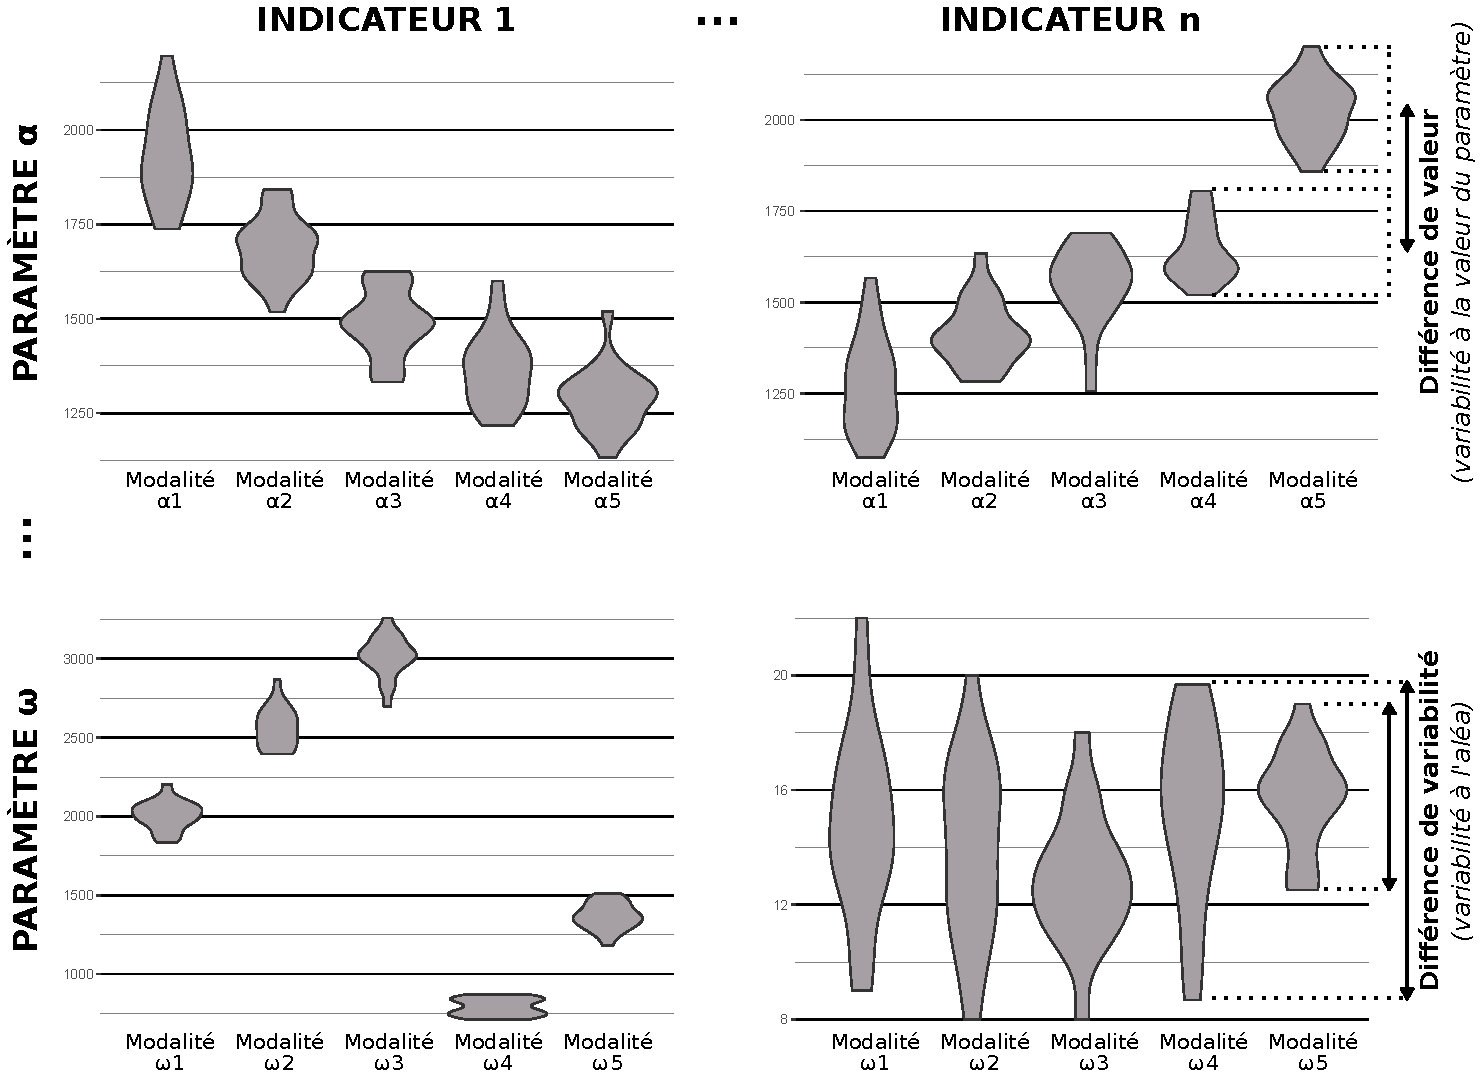
\includegraphics[width=\linewidth]{img/schema_violinplots_sensib.pdf}
	\caption[Construction et mise en page de planches graphiques dédiées à l'analyse visuelle de la sensibilité.]{Construction et mise en page de planches graphiques dédiées à l'analyse visuelle de la sensibilité de 5 modalités de $\upomega$ paramètres sur \textit{n} indicateurs.}
	\label{fig:exemple-visu-sensib}
\end{figure}
\clearpage


Ces planches permettent de lire une double information.
En premier lieu, la position relative des valeurs correspondant à chaque modalité permet de remarquer d'éventuelles influences des valeurs de paramètres sur les valeurs d'indicateur.
Dans le schéma, on représente ainsi les \og différences de valeur\fg{} qui expriment une variabilité à la valeur du paramètre (exemple en haut à droite).
Dans un second temps, et on y reviendra après (\cref{subsec:sensibilite-alea}), le choix des représentations en \textit{violin-plots} permet aussi d'étudier la variabilité interne des valeurs de paramètres testées sur chaque indicateur (exemple en bas à droite).
Les différences d'amplitude (sur l'axe des ordonnées) exprime ainsi les différentes variabilités dues à l'aléa : plus les \og violons\fg{} sont grands, plus l'indicateur varie selon les réplications pour la valeur de paramètre testée.

\paragraph{Normalisation.}
La normalisation des valeurs était indispensable lors du calcul de la sensibilité globale afin d'homogénéiser la variabilité des indicateurs.
Pourtant, sur un sous-ensemble de paramètres cette normalisation devient un frein à l'interprétation et à la lisibilité des analyses : les valeurs des différents indicateurs n'étant plus exprimés dans l'unité d'origine, il est difficile d'en faire un commentaire thématique.
L'analyse visuelle, sur les paramètres sélectionnés, sera ainsi présentée sur les valeurs brutes issues des simulations, et chaque graphique aura en conséquence un axe des ordonnées propre.
La logique est encore une fois la même que dans les classifications ascendantes hiérarchiques couramment pratiquées en géographie quantitative : on effectue la classification sur des valeurs normalisées, mais on représente souvent les profils des classes en revenant aux valeurs brutes.
\clearpage

\subsection{Sélection des paramètres à analyser.}
\begin{figure}[H]
	%\vspace{-2em}
	\centering
	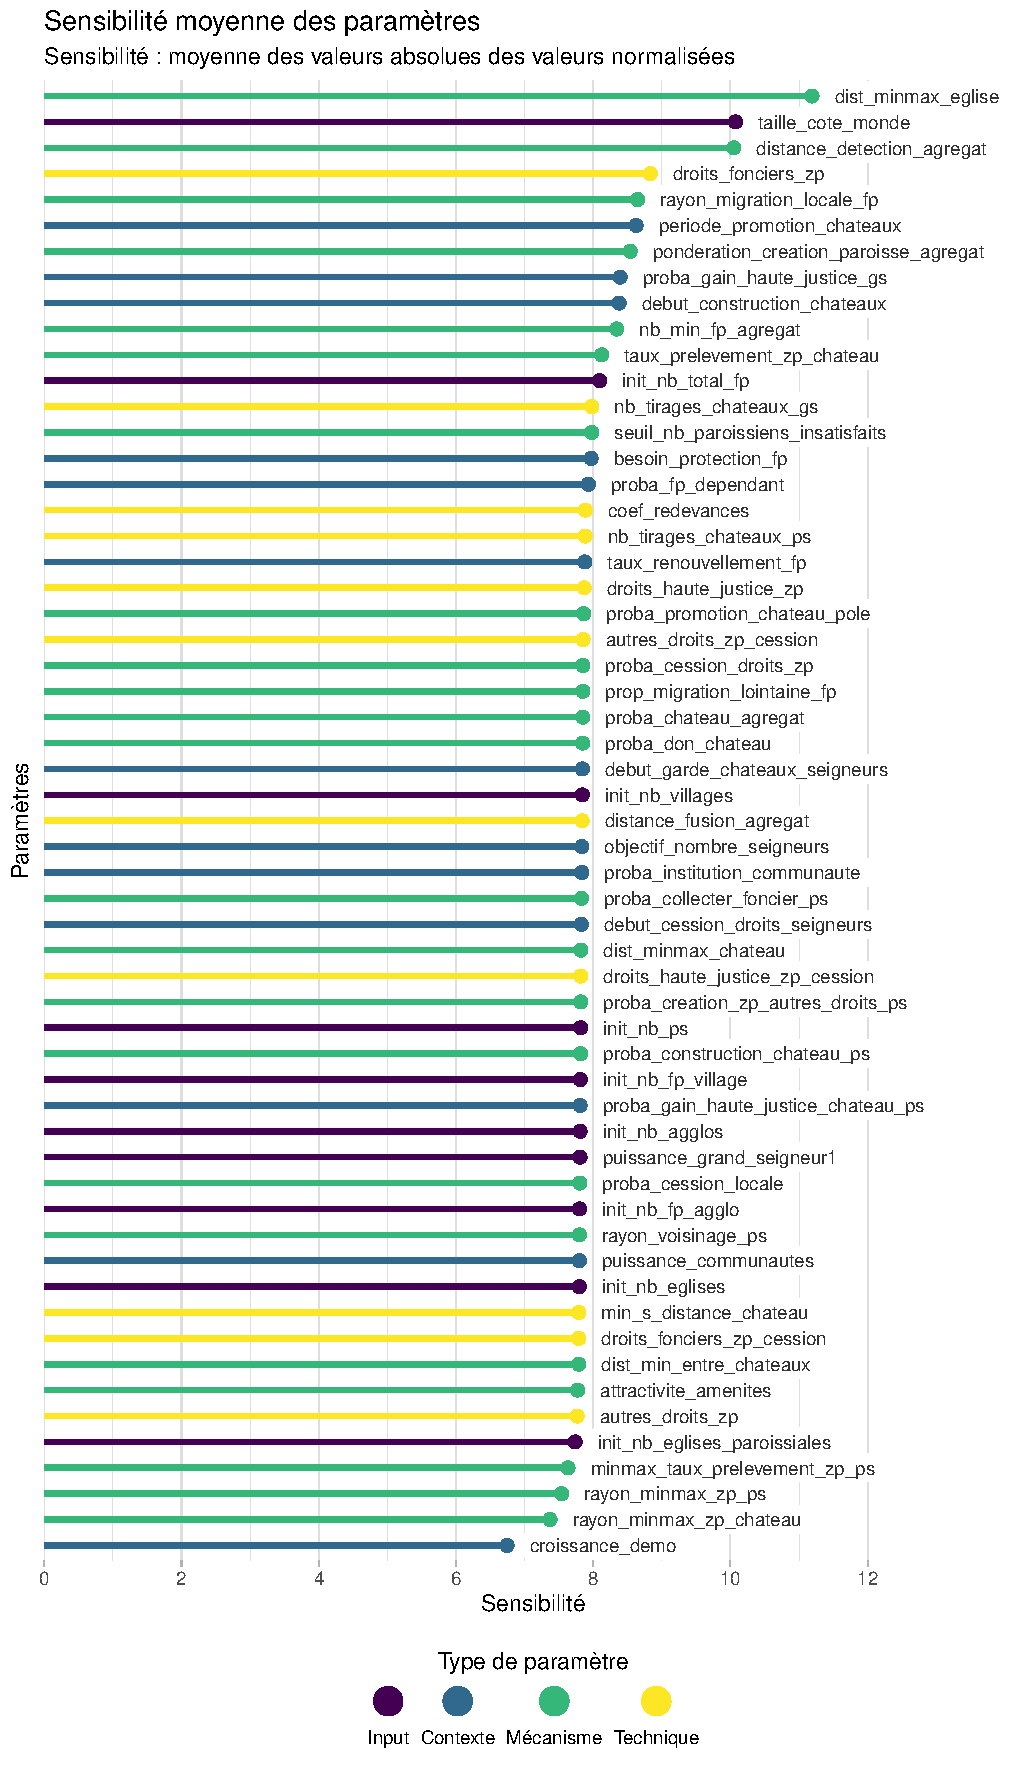
\includegraphics[width=.92\linewidth]{img/sensibilite_globale.pdf}
	\caption{Analyse de la sensibilité globale de tous les paramètres de \simfeodal{}.}
	\label{fig:sensibilite-globale}
\end{figure}
\clearpage

La \cref{fig:sensibilite-globale} présente les \og scores de sensibilité\fg{} de chacun des paramètres du modèle.
Ces paramètres sont classés par ordre descendant selon leur sensibilité globale, et la couleur précise la typologie des paramètres.

On constate tout d'abord que la sensibilité des paramètres est relativement peu dispersée : les valeurs abstraites de la sensibilité varient entre près de \og 7\fg{} et \og 11\fg{}, soit un écart maximal de 65\%.
%, là où on aurait pu imaginer que certains paramètres aient des sensibilités doublées, triplées, etc. par rapport à d'autres.
Cela indique que les paramètres ont tous une influence sur les sorties du modèle, influence qui est située dans le même ordre de grandeur.
Par extension, on note qu'aucun des paramètres testés ne présente une sensibilité véritablement faible.
Ce constat est renforcé en considérant que le paramètre le moins sensible globalement (\textsf{croissance\_demo}) a une influence réelle sur le modèle, pour avoir notamment été testé plus extensivement en parallèle de cette analyse de sensibilité (voir \cref{enc:scenario-croissance-demo}).
Pour le modélisateur, cette relative homogénéité des sensibilités est un résultat véritablement rassurant.
Cela nous prouve qu'aucun paramètre n'est inutile (dans le sens où il n'agirait pas, ou très peu, sur le modèle), et ne devrait par conséquent être supprimé du modèle si on recherchait une parcimonie plus importante à cette étape (dans le cas d'un paramètre ayant une faible influence par exemple).

Toujours à un niveau d'observation global, on peut remarquer que la sensibilité globale des paramètres ne semble pas liée aux types de paramètres.
Visuellement, on constate en effet qu'il ne semble pas y avoir de motif particulier dans le positionnement des types représentés par les couleurs.
En cela, le choix de mener l'analyse indistinctement sur tous les types de paramètres semble avoir été le bon.

En entrant dans le détail, on peut remarquer que trois paramètres se démarquent véritablement : les seuils de distance acceptables à l'église paroissiale la plus proche (\textsf{dist\_minmax\_eglise}), la dimension du monde simulé (\textsf{taille\_cote\_monde}) et le seuil de distance de détection des agrégats, en dessous duquel on considère que des foyers paysans peuvent former un agrégat (\textsf{distance\_detection\_agregat}).
Il est intéressant de noter que les valeurs par défaut de ces paramètres ont toutes été choisies avec une précaution particulière.
\begin{itemize}
	\item Le seuil de distance aux églises est un paramètre particulièrement complexe qui a donné lieu à de multiples allers-retours pour en fixer les valeurs.
	Sur la forme, c'est l'un des paramètres les plus \og qualitatifs\fg{} : il désigne une étendue spatiale qui varie au cours du temps de la simulation.
	Comme la satisfaction religieuse que ce paramètre conditionne a une importance majeure sur les migrations des foyers paysans (voir \cref{sssec:fixation-dissemination}), on pouvait s'attendre à ce qu'il se montre particulièrement sensible.
	\item Les dimensions du monde simulé ont donné lieu à un calibrage, par ajustement empirique, dont l'on a discuté au début de ce chapitre (\cref{sssec:calibrage-inputs}).
	On décrivait alors toutes les répercussions que ce changement avait provoqué, et il n'est pas surprenant que ce paramètre soit parmis les plus sensibles dans le modèle.
	\item La distance de détection des agrégats a été l'un des premiers paramètres implémenté dans le modèle, ajusté selon des valeurs empiriques.
	La valeur fixée (100 m) n'a pas évoluée depuis les premières versions du modèle.
	C'en est presque une constante et il est très enrichissant pour le modélisateur de découvrir que ce paramètre a une influence importante sur l'issue des simulations.
\end{itemize}

Au sein des paramètres qui suivent immédiatement ce trio, les ruptures sont moins nettes et l'on découpera donc ce continuum entre les paramètres situés en 10$^e$ et 11$^e$ position (\textsf{nb\_min\_fp\_agregat} et \textsf{taux\_prelevement\_zp\_chateau}), où l'on discerne visuellement un nouveau saut dans les valeurs de sensibilité.
Sur ces 57 paramètres, cette sélection en isole donc 10, auxquels on ajoute une sélection des trois paramètres ayant la plus forte sensibilité sur chacun des indicateurs.
Comme ces derniers sont en bonne partie redondants avec les autres sélections, on obtient finalement un total de 14 paramètres à analyser visuellement par la suite.
Ces paramètres, leur description complète ainsi que les valeurs testées sont présentées dans le \cref{tab:selection-parametres-anavis}.

\paragraph{Limites de cette approche de sélection.}
Avant de passer à l'analyse détaillée des paramètres isolés, il nous parait important de noter une limite substantielle de la méthode mise en place pour leur sélection.
La mesure choisie, consistant en une sensibilité normalisée, ne tient pas compte de l'étendue des valeurs de paramètres testées.
Ces étendues sont largement incommensurables, qui plus est quand il s'agit de comparer des paramètres numériques simples (la taille des côtés du monde simulé) à des paramètres plus qualitatifs (les seuils de distance évolutifs de la distance aux églises paroissiales).
On peut par exemple noter que dans les 10 paramètres jugés les plus sensibles, 4 portent sur des valeurs testés \og qualitatives\fg{} (étendues, variables au cours du temps, etc., voir p.~\pageref{par:etendue-parametres}), alors que ces paramètres ne représentent que 20\% de l'ensemble des paramètres testés.

Lors du choix des valeurs de paramètres à tester pour cette analyse de sensibilité (disponibles dans l'\cref{annexe:A}, \cref{annexe:A3}), certains paramètres auront forcément été testés sur des valeurs plus ou moins éloignées des valeurs par défaut issues du calibrage.
Cet éloignement se traduit forcément par des sensibilités mesurées très variables.
On peut illustrer ce biais en comparant un paramètre de stock simple qui se montre très sensible (la taille du monde simulé à nouveau) et un paramètre de ratio qui se situe lui tout en bas du classement (le taux de croissance démographique, \textsf{croissance\_demo}).
\begin{itemize}
	\item Pour le premier, les valeurs testées s'échelonne régulièrement entre 50 et 150 km.
	L'ordre de grandeur de ces valeurs est similaire, représentant une variation qui va environ de la division par deux à la multiplication par deux de la valeur par défaut (80 km).
	\item Pour le second, qui vaut 0\% par défaut, les valeurs testées sont de 0\%, 1.53\%, 3.72\%, 5.89\% et 12.89\%.
	Au regard du nombre de pas de temps, cela représente un doublement, un triplement, un quintuplement et enfin un décuplement de la population initiale, que l'on a fait covarier pour que la population finale soit systématiquement identique.
 	Vis-à-vis du paramètre précédent, l'étendue interprétée est plus large, consistant même en une activation ou non du mécanisme de croissance démographique.
 	En absolu, les 4 premières valeurs sont cependant très proches et on ne s'attend ainsi pas à ce qu'elles aient un effet majeur sur les sorties du modèle.	
\end{itemize}

Un autre exemple de cette incomparabilité des étendues concerne le choix des valeurs à tester pour les paramètres techniques.
Par définition, ceux-ci ont des valeurs qui ne représentent strictement rien d'un point de vue thématique.
Leur étendue acceptable est alors extrêmement difficile à évaluer, et on aura ainsi pu avoir tendance à effectuer de mauvais jugements sur les valeurs testées de ces paramètres.

Ces biais dans la comparabilité des valeurs de paramètres testées ont forcément influencé la sélection des paramètres à analyser.
En changeant les valeurs testées, le classement des paramètres aurait sans doute été largement altéré.
Dans l'incapacité de produire des valeurs de paramètres plus comparables, nous nous tiendrons toutefois à la sélection des paramètres \og les plus sensibles\fg{} effectuée dans cette partie.
Tous les paramètres peuvent toutefois être analysés individuellement, de manière interactive, dans la partie dédiée de la plateforme \simedb{} (\cref{fig:screenshot-simedb-sensib}).

%TODO : ICI !
\begin{figure}[H]
	\centering
	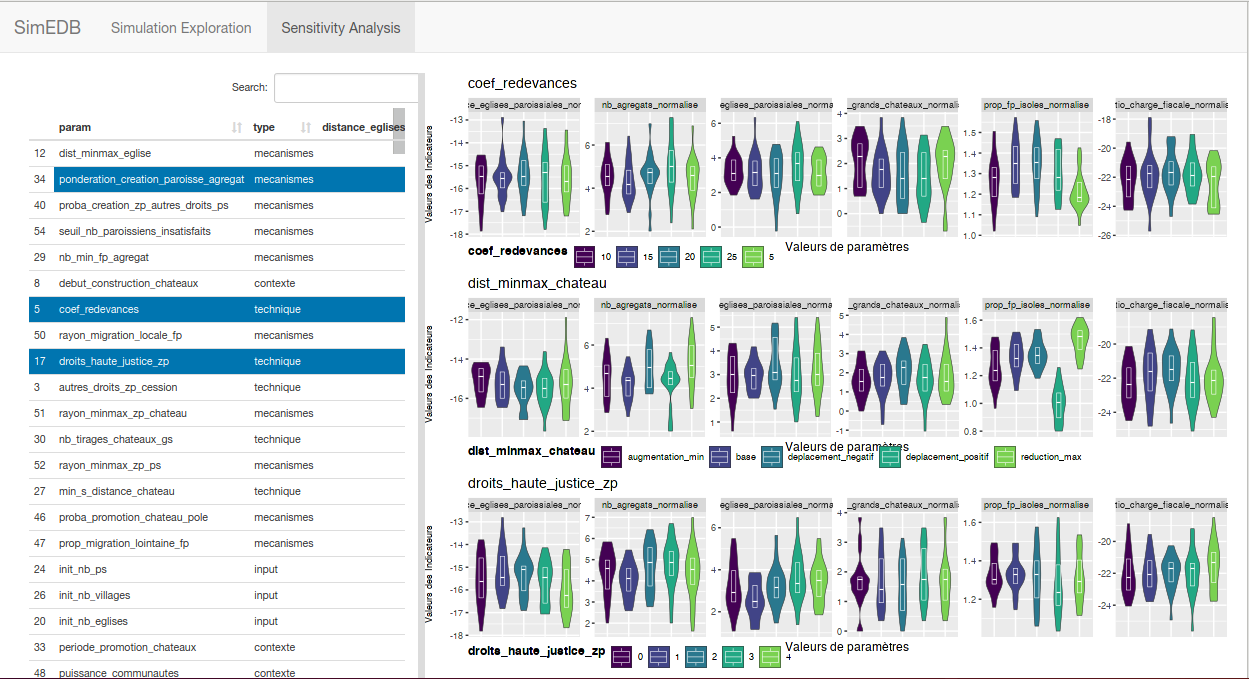
\includegraphics[width=\linewidth]{img/SimEDB_sensib.png}
	\caption[Partie de l'interface de \simedb{} dédiée à l'exploration visuelle des résultats de l'analyse de sensibilité de \simfeodal{}.]{Partie de l'interface de \simedb{} dédiée à l'exploration visuelle des résultats de l'analyse de sensibilité de \simfeodal{}.\\
	Interface accessible sur \href{https://simedb.cura.info/analyse-sensibilite}{https://simedb.cura.info/analyse-sensibilite}.}
	\label{fig:screenshot-simedb-sensib}
\end{figure}

\clearpage
\begin{table}[p]
\centering
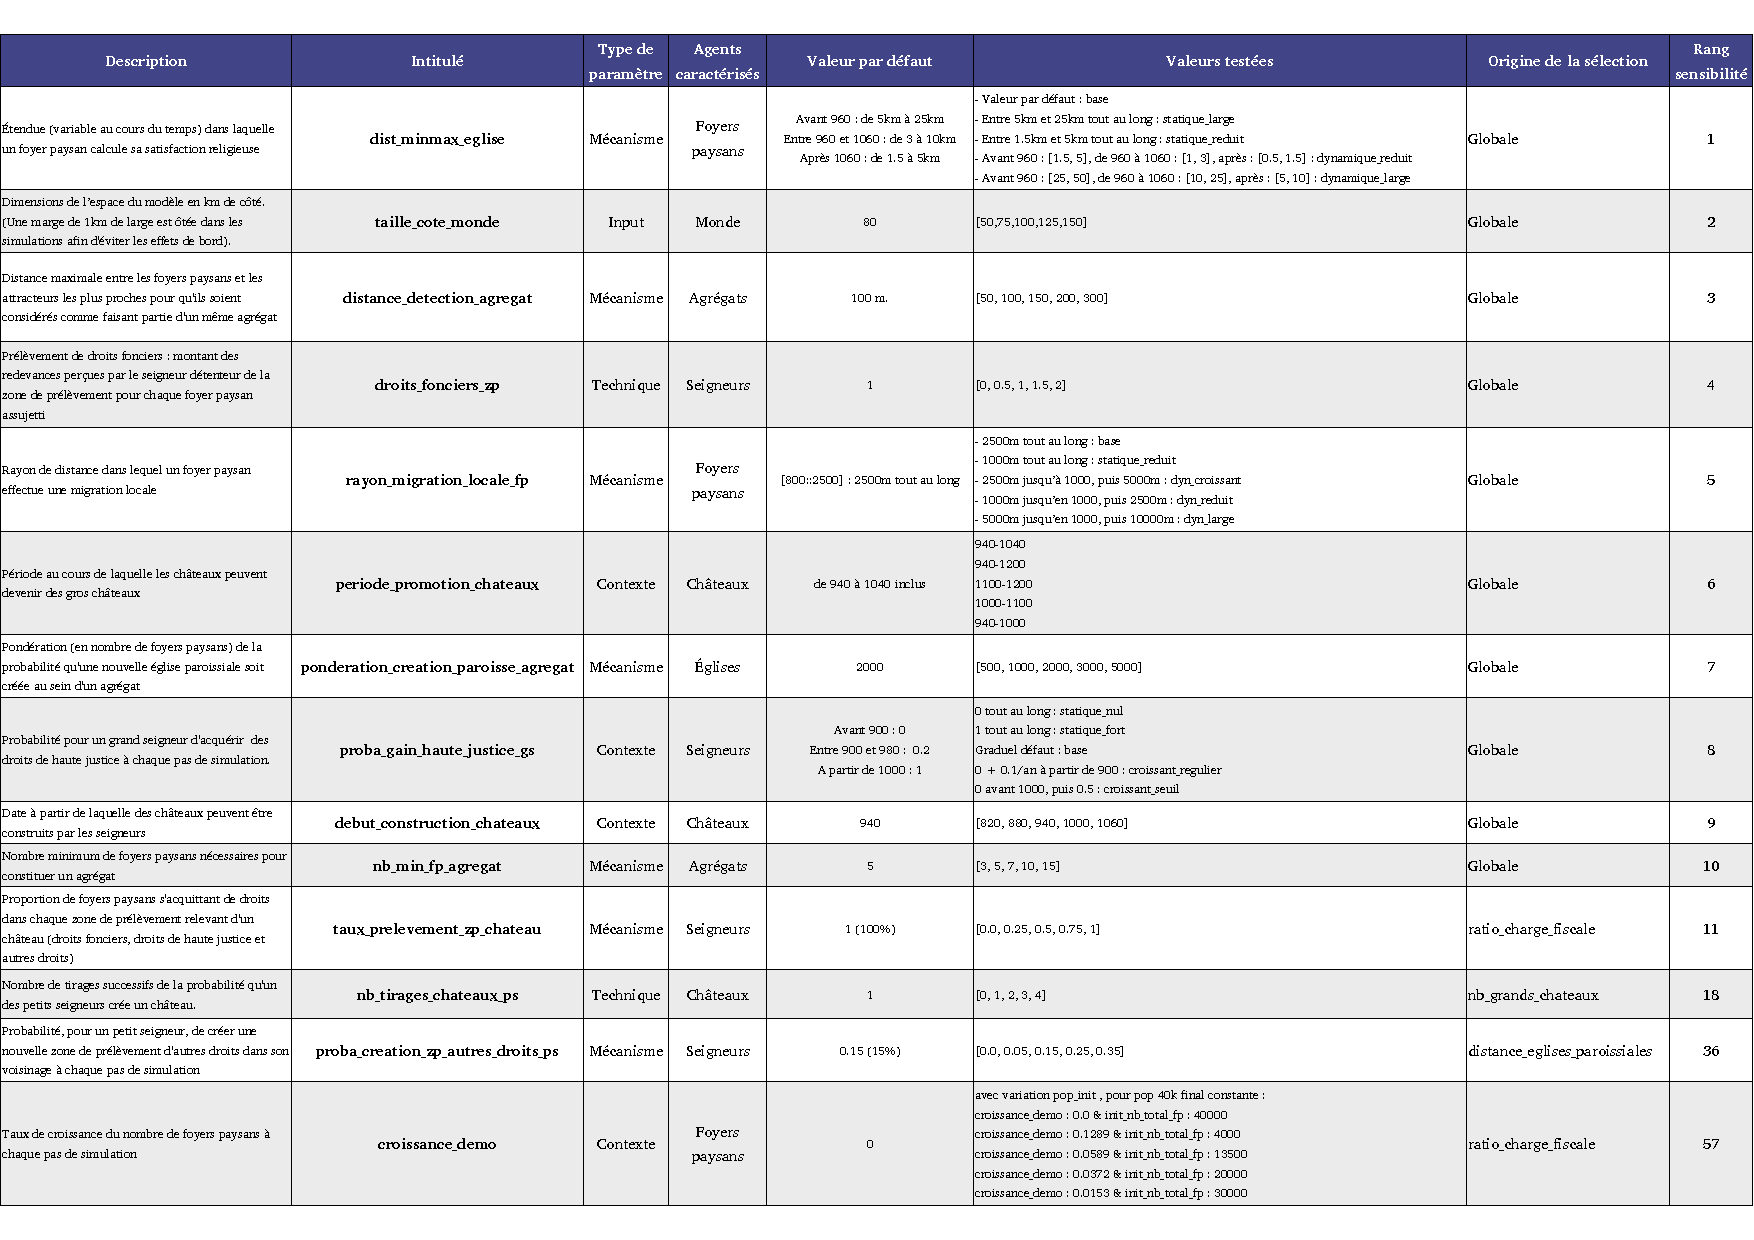
\includegraphics[width=.91\textheight, angle=90, origin=c]{img/Parametres.pdf}
\caption{Paramètres sélectionnés pour l'analyse visuelle.}
\label{tab:selection-parametres-anavis}
\end{table}
\clearpage

\subsection{Évaluation visuelle de la sensibilité}

%\bigskip
%\begin{mdframed}[backgroundcolor=black!5,footnoteinside=false]
%	Les graphiques présentés dans la suite de ce chapitre ne concernent que les paramètres sélectionnés lors de l'analyse quantitative globale.
%	Tous les paramètres peuvent toutefois être analysés individuellement, de manière interactive, dans la partie dédiée de la plateforme \simedb{} : \hl{Mettre un lien direct}.
%\end{mdframed}

Plutôt que de mener l'évaluation de la sensibilité des paramètres sélectionnés de manière linéaire, paramètre après paramètre, nous présentons ces derniers organisés par thématique c'est-à-dire selon les types d'agents concernés par chacun d'entre eux.

\subsubsection{Paramètres liés au monde simulé}

\begin{figure}[H]
	\centering
	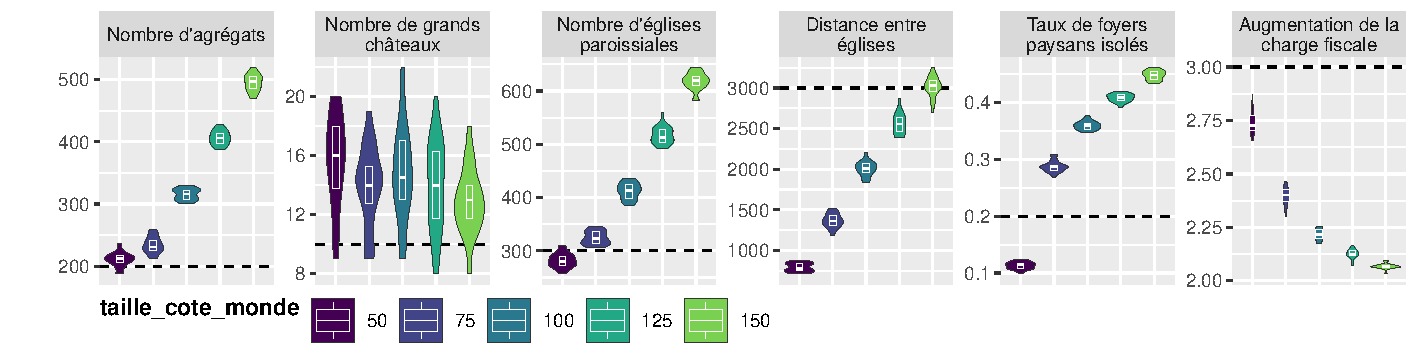
\includegraphics[width=\linewidth]{img/sensib/sensibilite_taille_cote_monde.pdf}
	\caption{Sensibilité à la taille du monde simulé.}
	\label{fig:sensib-monde}
\end{figure}

%Le paramètre régissant la taille du monde simulé est le seul des \textit{inputs} présent dans la sélection.

Le paramètre régissant la taille du monde simulé (\textsf{taille\_cote\_monde}) est un paramètre majeur qui affecte la totalité des indicateurs étudiés, comme la \cref{fig:sensib-monde} permet de le constater.
Quand la taille du monde simulé augmente, le nombre d'agrégats, d'églises paroissiales, la distance moyenne entre églises paroissiales et le taux de foyers paysans augmente aussi.
Au contraire, la pression fiscale varie de façon inverse : quand la taille du monde simulé augmente, elle diminue.
On ne constate pas d'effet direct ou linéaire sur le nombre de grands châteaux, qui ne semblent pas être directement sensibles à la taille du monde.
Les différences visuelles de position semblent surtout influencées par la forte variabilité liée à l'aléa que l'on constate sur cet indicateur de sortie de simulation.

Ces résultats sont assez intuitifs : plus le monde est restreint, plus les foyers paysans sont proches les uns des autres.
Cela entraîne premièrement une concentration plus forte, mais aussi un nombre d'agrégats plus faible : au lieu d'être dispersés en une multitude de petits agrégats (500 en moyenne avec un monde de 150 km de côté), les foyers paysans se concentrent dans un nombre restreint d'agrégats (200 quand le côté est de 50 km), de superficie vraisemblablement supérieures par les effets des mécanismes de fusion des agrégats.
En effet, quand la superficie d'ensemble est plus faible, toutes choses égales par ailleurs concernant le nombre et le rayon des zones de prélèvement, on assiste nécessairement à une superposition plus importante de ces zones.
La charge fiscale des foyers paysans s'en retrouve fortement affectée.

Un effet de ce paramètre nous paraît légèrement contre-intuitif : avec une surface plus importante, il est entièrement logique que la distance entre les églises augmente, puisque celles-ci sont forcément plus dispersés dans un monde plus large.
Pourtant, le nombre d'églises paroissiales croît aussi avec la superficie du monde simulé, ce qui ne nous semble pas découler directement des règles de création/promotion de nouvelles églises paroissiales.
On peut interpréter ce comportement comme une conséquence imprévue et non linéaire de la dispersion des foyers paysans au sein de petits agrégats.
De petites églises paroissiales sont mécaniquement créées ou promues en plus grand nombre dans les zones faiblement peuplées (petits agrégats proches du seuil minimal), là où la création d'une paroisse est moins coûteuse (en termes de nombre de foyers paysans requis) qu'au sein des agrégats plus importants.
En renforçant le nombre d'agrégats, le paramètre de taille du monde simulé agit ainsi de manière indirecte sur le nombre d'églises paroissiales.

\subsubsection{Paramètres liés aux foyers paysans et agrégats \label{subsubsec:sensib-fp}}

Les foyers paysans (et les agrégats de population qui résultent de leur concentration) sont, par hypothèse, les agents les plus déterminants dans l'évolution des structures spatiales observées dans \simfeodal{}.
À ce titre, il est attendu (et sécurisant en termes de validation interne) que les paramètres contrôlant leurs mécanismes propres aient une influence nette sur les indicateurs de sortie analysés.

\paragraph{Foyers paysans.}
Les trois paramètres, spécifiquement liés aux foyers paysans, les plus sensibles (\cref{fig:sensib-fp-1,fig:sensib-fp-2,fig:sensib-fp-3}), embrassent trois aspects bien différents des mécanismes gérant le comportement des foyers paysans.

\begin{figure}[H]
	\centering
	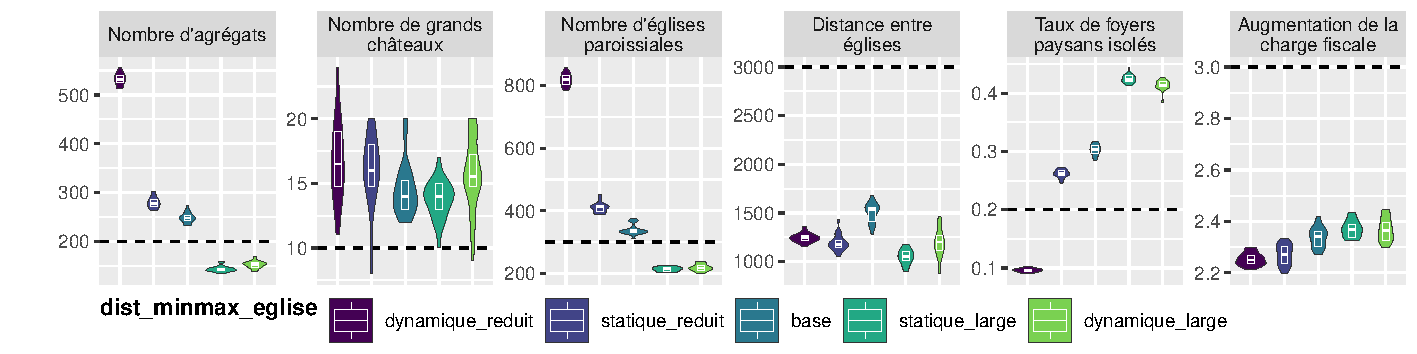
\includegraphics[width=\linewidth]{img/sensib/sensibilite_dist_minmax_eglise.pdf}
	\caption[Sensibilité du paramètre \textsf{dist\_minmax\_eglise}.]{Sensibilité du paramètre \textsf{dist\_minmax\_eglise}.\\
\textit{	N.B. : Pour les paramètres à valeurs qualitatives, l'ordre de présentation des valeurs est déterminant pour l'analyse visuelle qui en sera faite.
	Pour ces paramètres, l'ordre suivi est \textit{ad hoc} et subjectif et peut être assimilé à un ordre croissant, par exemple dans l'amplitude des étendues.}}
	\label{fig:sensib-fp-1}
\end{figure}

Le premier de ces paramètres (\cref{fig:sensib-fp-1}), qui est aussi le plus sensible du modèle, joue sur la satisfaction religieuse des foyers paysans.
Notons déjà que le calibrage de ce paramètre semble efficace : au moins sur les quatre premiers indicateurs, c'est la valeur par défaut dans le modèle qui approche le plus les objectifs fixés.
En matière d'interprétation, le fait que ce paramètre ait une influence sur les indicateurs de sortie du modèle est attendu et intuitif.
La satisfaction religieuse que ce paramètre conditionne, est en effet, intentionnellement l'un des éléments majeurs du modèle.

Pourtant, l'ampleur de cette influence est un peu plus forte qu'on aurait pu le penser au vu des mécanismes et résultats principaux du modèle.
Dans la \cref{fig:results-fp-satisfaction} qui présentait l'évolution de la satisfaction des foyers paysans, on remarquait que la composante \og protection\fg{} était la plus importante de la satisfaction globale.
On aurait donc pu s'attendre, au regard des mécanismes implémentés, à ce que les paramètres liés à la satisfaction protection aient une sensibilité supérieure à celui-ci.

Pour ce paramètre qui régit les seuils de distance acceptables à l'église paroissiale la plus proche, on peut émettre l'hypothèse que les valeurs testées biaisent la mesure de la sensibilité globale.
Ces valeurs sont qualitatives (étendues plus ou moins importantes, variables ou non au cours du temps, cf. le \cref{tab:selection-parametres-anavis}), ont une large influence sur les aspects liés à la concentration des foyers paysans, et leur action sur les autres indicateurs est moins linéaire et prévisible.

Plus les étendues testées sont restreintes (modalités \og dynamique\_reduit\fg{} et \og statique\_reduit\fg{}), plus le nombre d'agrégats et de foyers paysans isolés est important.
Pour ceux-là, la satisfaction religieuse joue à ce moment là le rôle limitant et \og force\fg{} les foyers paysans à migrer à proximité d'églises paroissiales.

\begin{figure}[H]
	\centering
	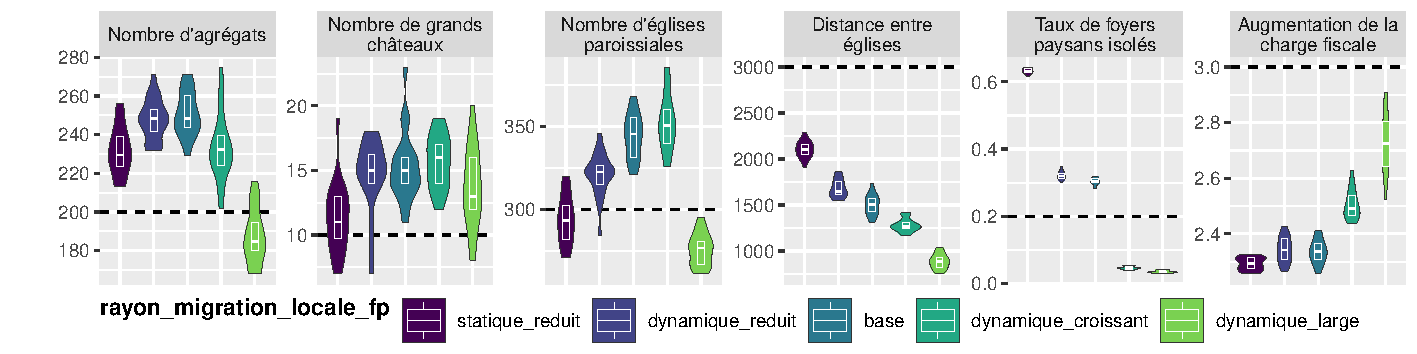
\includegraphics[width=\linewidth]{img/sensib/sensibilite_rayon_migration_locale_fp.pdf}
	\caption{Sensibilité du paramètre \textsf{rayon\_migration\_locale\_fp}.}
	\label{fig:sensib-fp-2}
\end{figure}

Cette migration, au moins pour l'aspect local, est largement influencée par le second paramètre de la sélection : le rayon maximal de migration locale des foyers paysans (\cref{fig:sensib-fp-2}). 
Celui-ci n'est pas une étendue, mais un rayon maximum qui peut changer au cours du temps (valeurs \og dynamiques\fg{}).
Dans le modèle calibré, ce rayon est fixe au cours du temps (2 500 m, modalité \og base\fg{}).
Dans des versions précédentes du modèle, les valeurs de ce paramètre augmentaient au cours du temps\footnote{
	Reproduisant ainsi \textit{in silico} la diminution des coûts de distance-temps qui témoignent de l'intégration d'un système de peuplement.
}, et on a voulu tester l'influence de l'évolution de ces valeurs (modalités \og dynamique\_reduit\fg{} et \og dynamique\_croissant\fg{}) ainsi que d'augmentations et diminutions du rayon (modalités de type \og reduit\fg{} par opposition à \og croissant\fg{} et \og large\fg{}).

Ce paramètre a notamment un rôle déterminant sur la concentration des foyers paysans, puisque selon les valeurs éprouvées, cet indicateur peut passer en moyenne de plus de 60\% à moins de 5\%.
Les effets sur le nombre d'agrégats, de grands châteaux et d'églises paroissiales ne sont pas directement linéaires.
C'est un exemple typique de paramètre qui régit un mécanisme dont les interactions avec les autres suit des effets de seuils.
Sur les indicateurs de sortie, cela résulte en des tendances diverses selon l'ordre de grandeur des seuils empruntés.

\begin{figure}[H]
	\centering
	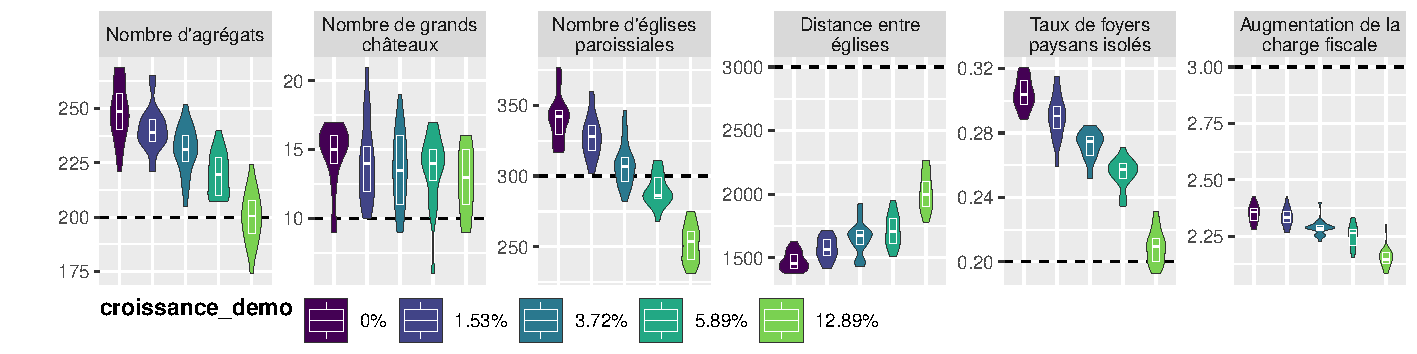
\includegraphics[width=\linewidth]{img/sensib/sensibilite_croissance_demo.pdf}
	\caption{Sensibilité du paramètre \textsf{croissance\_demo}.}
	\label{fig:sensib-fp-3}
\end{figure}

Le paramètre de croissance démographique régit un mécanisme particulier dans le modèle, puisque par hypothèse, on a choisi de considérer une population stable dans le déroulement du modèle.

Ce paramètre est considéré comme relevant du contexte, mais aurait également entièrement sa place parmi les \textit{inputs} tant son importance thématique est majeure.
La très faible sensibilité globale de ce paramètre (\cref{fig:sensibilite-globale}), ne nous paraît pas représentative de son influence effective tant l'analyse visuelle de son influence sur les indicateurs de sortie (\cref{fig:sensib-fp-3}) montre un effet direct sur tous les indicateurs présentés (à l'exception du nombre de grands châteaux).

On peut constater que plus le taux de croissance est élevé, plus le nombre d'agrégats est faible, de même que le taux de foyers paysans isolés.
Sur les deux paramètres précédents (\cref{fig:sensib-fp-1,fig:sensib-fp-2}), de même que plus globalement, ces deux indicateurs sont pourtant le plus souvent opposés : quand le nombre d'agrégat augmente, le taux de foyer paysans isolés diminue.

L'influence de ce paramètre est extrêmement intéressante pour le modèle tant ce paramètre permet d'approcher des objectifs de ces indicateurs qui sont tous deux dépassés alors qu'opposés.
On notera par exemple que parmi les valeurs de croissance démographique testées, la plus forte (12.80\%) permet un excellent ajustement du nombre d'agrégats et du taux de foyers paysans isolés, deux objectifs majeurs dans l'évaluation de \simfeodal{}.
L'\cref{enc:scenario-croissance-demo} illustre une démarche d'exploration plus poussée de ce paramètre.
\clearpage

\begin{encadre}{Un scénario thématique pour tester l'hypothèse de croissance démographique}{scenario-croissance-demo}
	\renewcommand{\thempfootnote}{\alph{mpfootnote}}	
L'envie de mener des \og scénarios thématiques\fg{} a émergé très tôt dans la conception du modèle \simfeodal{}.
L'idée était de pouvoir tester des hypothèses différentes quant aux grands faits stylisés mobilisés dans le modèle.
Ces versions alternatives permettraient d'éprouver la validité du modèle, et donc des logiques sur lequel il repose, en l'adaptant à d'autres régions où les processus ont été différents voire inexistants.

\vspace*{1em} À ce jour, une quinzaine de scénarios de tels types ont été conçus, implémentés et simulés.
La temporalité plus large de ce projet de recherche par rapport à celle de ce travail de thèse fait que l'analyse des résultats de ces scénarios et des résultats thématiques qu'ils engendrent est encore en cours par l'ensemble de l'équipe de \simfeodal{}.

\vspace*{1em} Dans cet encadré, nous présentons toutefois un scénario, qui permet de revenir sur un élément majeur du modèle tel qu'il a été conçu.
Cet élément est l'absence de prise en compte de croissance démographique, quand bien même empiriquement, on sait qu'il y a eu une croissance.
Pour tester les effets d'une telle croissance sur les sorties du modèle, on a procédé presque toute chose égale par ailleurs : la quasi-totalité des paramètres n'a pas été modifié, et le modèle n'a donc pas été re-calibré pour être adapté à ce mécanisme, nouveau et majeur, qui a été implémenté.
Seule exception : pour que l'état final du scénario soit comparable à l'état final de la version calibrée, il fallait que les populations soient comparables.
De même que l'on a fait varier le taux de croissance démographique, on a donc aussi fait varier la population initiale du modèle, afin que la population atteigne 40 000 foyers paysans en fin de simulation.

\vspace*{1em} Il y a eu trois scénarios conçus pour éprouver l'influence de taux variables de croissance démographique (D1, D2 et D3).
On n'en présente ici qu'un seul, par soucis de brièveté.
Ce scénario, intitulé \og D2\fg{}, est celui dont les résultats sont les plus intéressants.
Dans ce scénario, le taux de croissance démographique est fixé à 12.89\%, ce qui permet de faire passer une population initiale de 4 000 foyers paysans à 40 000 en fin de simulation.
Cela correspond donc à un décuplement de la population entre 800 et 1200, jugé non aberrant par les thématiciens.

\begin{table}[H]
	\captionsetup{singlelinecheck=off}
	\centering
	\small
	\resizebox{\textwidth}{!}{%
	{\renewcommand{\arraystretch}{1.1}%
		\begin{tabular}{|p{3.25cm}|p{2.1cm}|p{2cm}|p{1.75cm}|p{1.75cm}|}
			\hline
			\textbf{Indicateur} & \textbf{Valeur} \textbf{attendue} & \textbf{Valeur de référence} & \textbf{Moyenne} & \textbf{Médiane} \\ \hline
			\textit{Agrégats} & \textit{200} & 249 & 198 & 199 \\ \hline
			\textit{Gros châteaux} & \textit{10} & 15 & 12 & 12 \\ \hline
			\textit{Églises paroissiales} & \textit{300} & 348 & 252 & 253 \\ \hline
			\textit{Distance moyenne entre églises} & \textit{3 000 m} & 1 459 m & 1 988 m & 1 975 m \\ \hline
			\textit{Part de foyers paysans isolés} & \textit{20 \%} & 30 \% & 21 \% & 21 \% \\ \hline
			\textit{Augmentation de la charge fiscale des foyers paysans} & \textit{x 3} & x 2.4 & x 2.6 & x 2.6 \\ \hline
	\end{tabular}}}
	\caption[Valeurs des indicateurs numériques du scénario D2 en fin de simulation.]{Valeurs des indicateurs numériques du scénario D2 en fin de simulation.
	\small
	\textit{Les valeurs de référence correspondent aux moyennes obtenues dans la version calibrée de \simfeodal{}, sans croissance démographique donc.}}
	\label{tab:results-D2}
\end{table}
\smallskip

\vspace*{1em} Les résultats agrégés de ce scénario (\cref{tab:results-D2}) sont globalement satisfaisants, et même davantage que ceux de la version calibrée : le nombre d'agrégats en fin de simulation et la part de foyers paysans isolés sont presque parfaitement ajustés aux valeurs attendues fixées empiriquement.
Le nombre de grands châteaux et l'augmentation de la charge fiscale sont aussi plus proches des attentes, bien que d'une manière moins franche.
Seul point négatif : les églises paroissiales sont beaucoup moins nombreuses dans ce scénario que dans la version de référence, et trop faibles désormais au regard des valeurs attendues.

\vspace*{1em} En regardant le détail de la structure, et notamment relative aux indicateurs de sortie relatifs aux agrégats (\cref{fig:scenario-D2-agregats}), on constate qu'en matière de hiérarchisation du système, les résultats de ce scénario sont aussi meilleurs que ceux de la version de base (\cref{fig:results-nb-agregrats,fig:results-rt-agregats}).
La croissance du nombre d'agrégats y est assez régulière, contrairement à la version calibrée (\cref{fig:results-nb-agregrats}) où l'évolution était très faible jusqu'en 1060.
Plutôt que d'insuffler un changement de tendance, les mécanismes exogènes (960 et 1060) ne font qu'accélerer un processus déjà actif.

On note aussi que l'organisation hiérarchique des agrégats, et son évolution, est bien plus proche des formes connues sur les sociétés contemporaines.
Dans la version calibrée du modèle (\cref{fig:results-rt-agregats}), la courbe conservait un \og coude\fg{} important, tandis qu'ici, on note que l'évolution tend vers un redressement de la pente de la courbe rang-taille.
En cela, l'organisation hiérarchique tend vers le modèle log-normal observé empiriquement sur de très nombreux systèmes (\textcite{cura_old_2017} par exemple).

\begin{figure}[H]
	\centering
	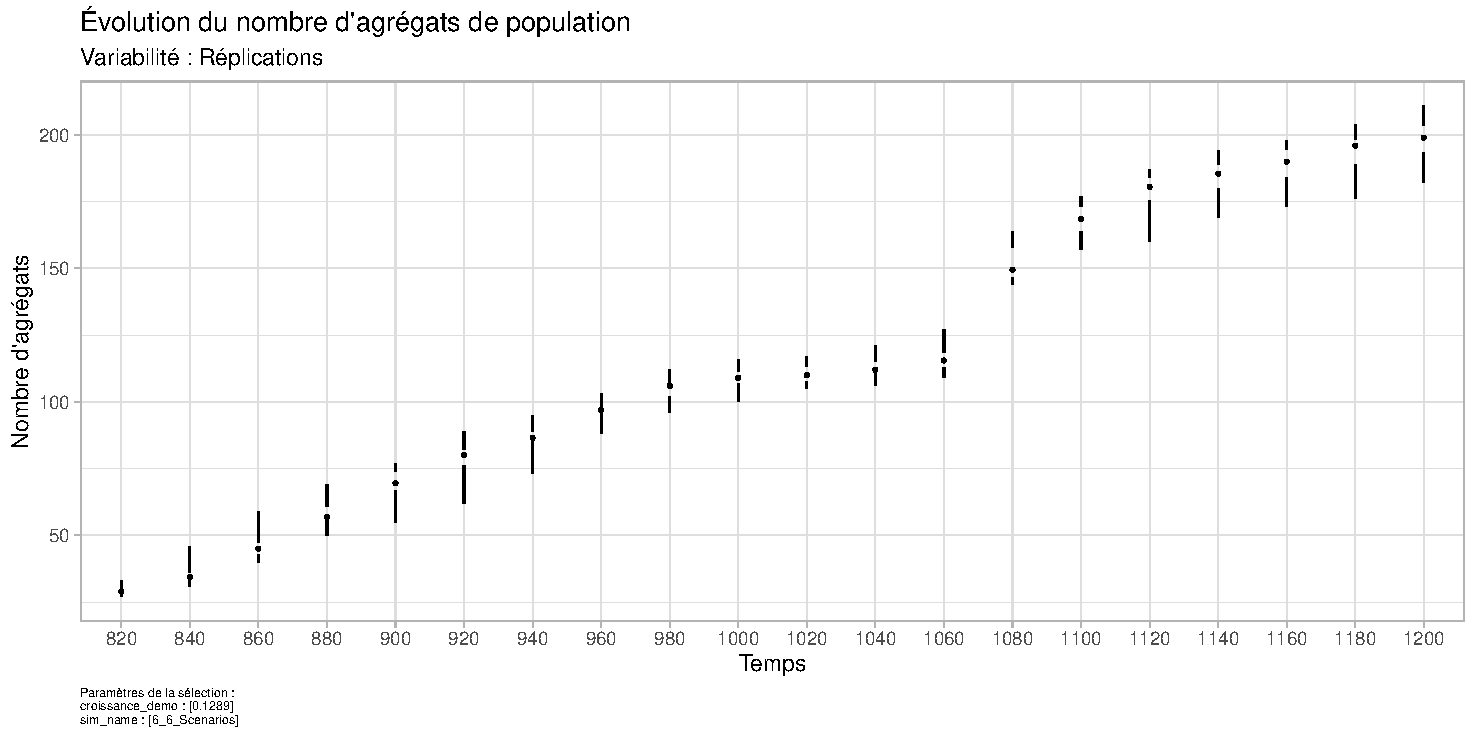
\includegraphics[width=\linewidth]{img/Agregats_Nb_D2.pdf}
	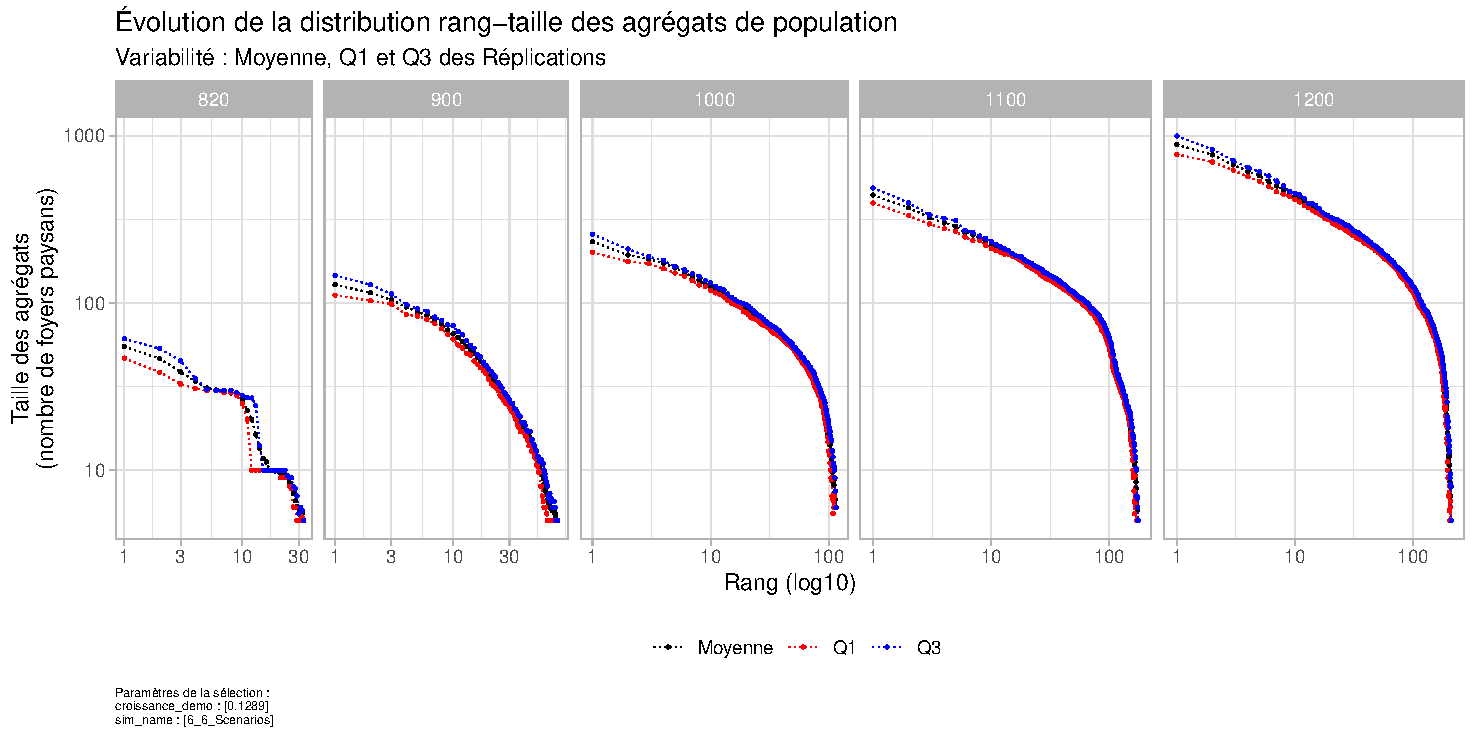
\includegraphics[width=\linewidth]{img/Agregats_RT_D2.pdf}
	\caption{Nombre et organisation des agrégats dans le scénario D2.}
	\label{fig:scenario-D2-agregats}
\end{figure}

Nous ne détaillerons pas les autres résultats de ce scénario D2, par ailleurs d'ores et déjà explorables dans la plateforme \simedb{} (\href{https://simedb.cura.info/6.6vD2}{https://simedb.cura.info/6.6vD2}), et nous contenterons d'affirmer que ce scénario répond mieux à une majorité des attentes identifiées pour \simfeodal{}.
C'est particulièrement étonnant dans la mesure où le modèle n'a jamais été conçu dans l'optique de remplacer la stabilité démographique par de la croissance, et n'a pas non plus été calibré à cet effet.
Sans perdre de vue les biais que l'implémentation informatique de mécanismes peut apporter vis-à-vis des processus modélisés, on notera tout de même qu'il est, thématiquement et méthodologiquement, très intéressant que les interactions entre mécanismes de \simfeodal{} s'ajustent mieux quand de la croissance démographique est mise en place.
Cela nous semble constituer un résultat majeur de ce scénario, et de \simfeodal{} plus globalement : sans mettre en place de mécanisme de croissance démographique, les objectifs thématiques à atteindre semblent inaccessibles, alors qu'une version même naïve et non calibrée d'un tel mécanisme permet déjà de répondre bien davantage aux objectifs formalisés.

%\cref{fig:scenario-D2-fp-migration}
%\begin{figure}[H]
%	\centering
%	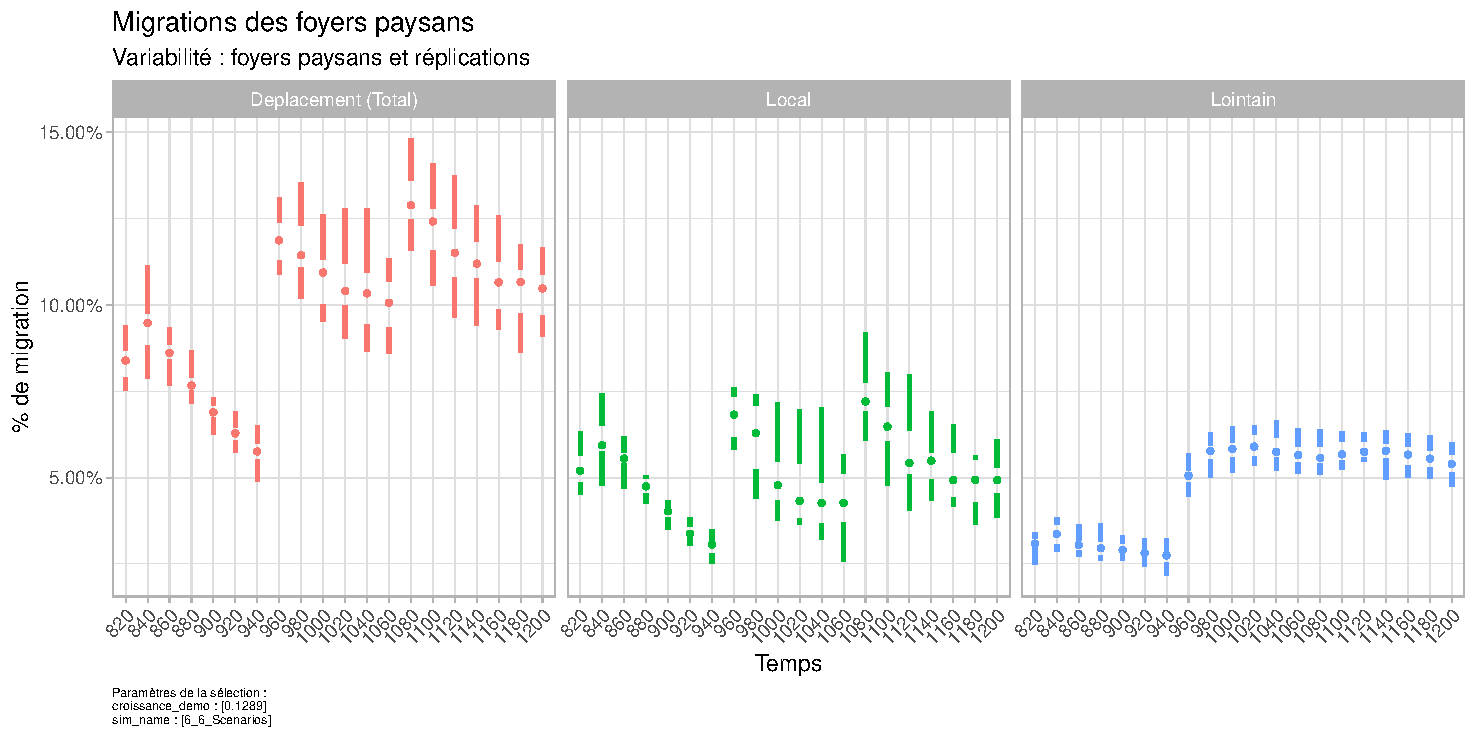
\includegraphics[width=\linewidth]{img/FP_TypeDeplacements_D2.pdf}
%	\caption{Évolution des migrations des foyers paysans dans le scénario D2.}
%	\label{fig:scenario-D2-fp-migration}
%\end{figure}
\smallskip
\end{encadre}

\paragraph{Agrégats de population.}

Les deux paramètres agissant sur la définition des agrégats (paramètres \textsf{distance\_detection\_agregat} et \textsf{nb\_min\_fp\_agregat}) sont très comparables et agissent de manière symétriquement opposée sur les indicateurs de sortie (\cref{fig:sensib-agregats}).

\begin{figure}[H]
	\centering
	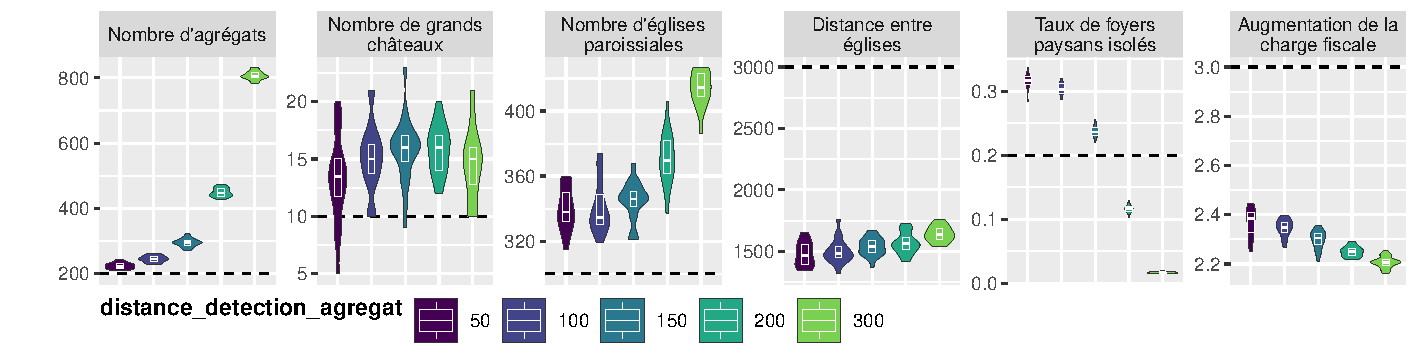
\includegraphics[width=\linewidth]{img/sensib/sensibilite_distance_detection_agregat.pdf}
	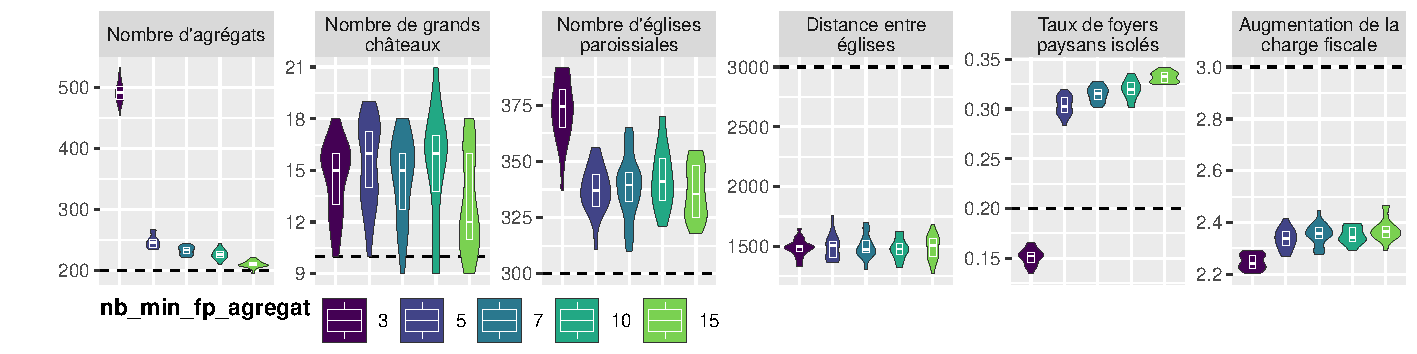
\includegraphics[width=\linewidth]{img/sensib/sensibilite_nb_min_fp_agregat.pdf}
	\caption{Sensibilité des paramètres liés aux agrégats.}
	\label{fig:sensib-agregats}
\end{figure}

Sans surprise, leur effet est largement circonscrit aux indicateurs relatifs aux foyers paysans (à l'exception inattendue des églises paroissiales, sans doute pour les mêmes raisons que le paramètre de taille du monde simulé), mais il est intéressant de noter leur extrême sensibilité.

On constate ainsi que des variations relativement fines de ces paramètres\footnote{
	Des distances de quelques dizaines/centaines de mètres de plus ou moins au regard des 80 kilomètres de côté du monde simulé pour le premier paramètre ; quelques foyers paysans de plus ou de moins pour constituer un agrégat dans le second paramètre, relativement aux 40 000 foyers paysans que compte le modèle\ldots
} aboutissent sur des variations plus que linéaires, et d'ordres de grandeurs quasi-différents sur le nombre d'agrégats (800 au maximum sur le premier paramètre, contre 200 au minimum) et le taux de foyers isolés (de plus de 30\% à moins de 2\% sur le même paramètre).

Les variations présentées dans la figure indique que les valeurs par défaut (100 m et 5 foyers paysans) sont au moins dans des intervalles assez sensés au regard des objectifs poursuivis.
Cela nous indique qu'il serait possible de jouer plus finement sur les valeurs de ces paramètres pour améliorer le calibrage de \simfeodal{}.

\subsubsection{Paramètres liés aux seigneurs et châteaux \label{sssec:sensib-params-seigneurs}}

Les paramètres liés aux seigneurs et aux châteaux (les premiers construisant les seconds) sont les plus nombreux du modèle et il est attendu qu'ils soient assez sensibles.
Ce sont en effet les paramètres qui régissent les mécanismes qui façonnent le monde dans lequel les foyers paysans auront à évoluer.

\paragraph{Seigneurs.}

La \cref{fig:sensib-seigneurs} présente les quatre paramètres sélectionnés liés aux seigneurs et aux châteaux :
\textsf{droits\_fonciers\_zp}, \textsf{proba\_gain\_haute\_justice\_gs}, \textsf{taux\_prelevement\_zp\_chateau} et \textsf{proba\_creation\_zp\_autres\_droits\_ps}.

\begin{figure}[H]
	\centering
	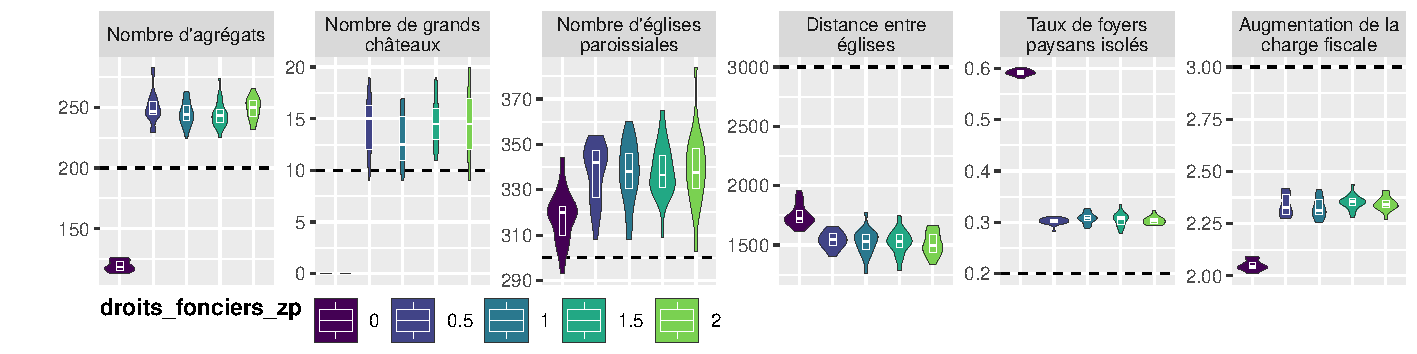
\includegraphics[width=\linewidth]{img/sensib/sensibilite_droits_fonciers_zp.pdf}
	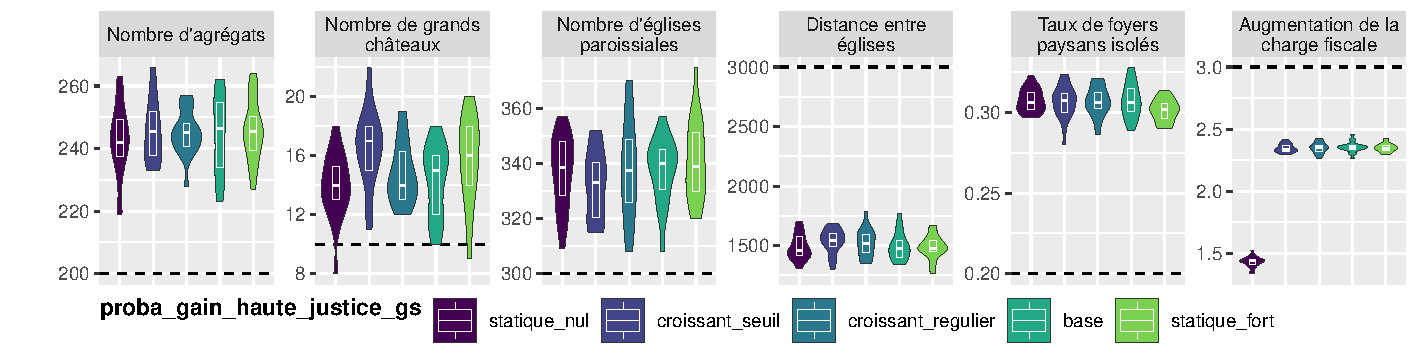
\includegraphics[width=\linewidth]{img/sensib/sensibilite_proba_gain_haute_justice_gs.pdf}
	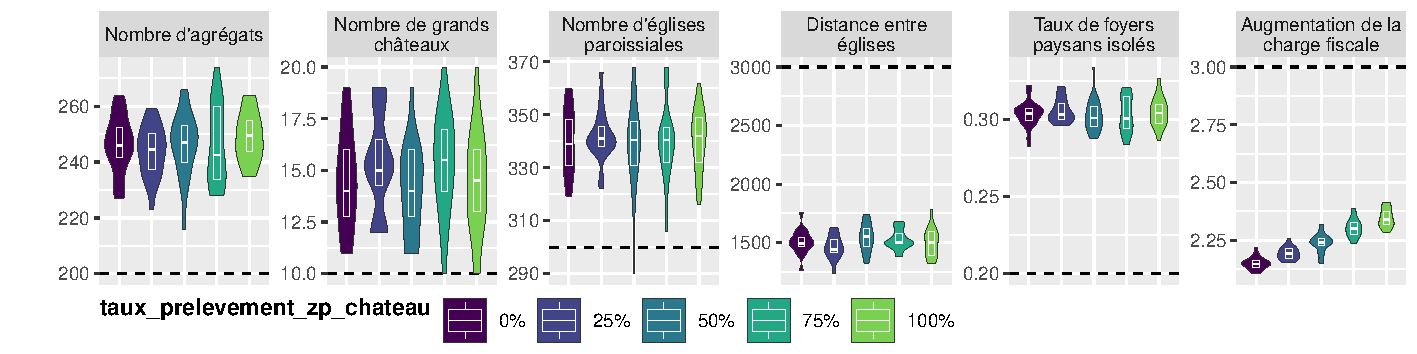
\includegraphics[width=\linewidth]{img/sensib/sensibilite_taux_prelevement_zp_chateau.pdf}
	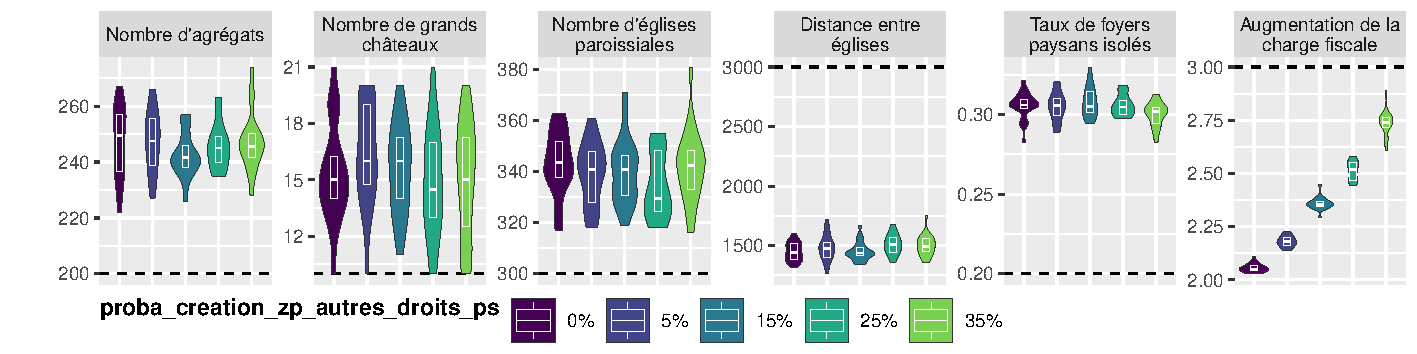
\includegraphics[width=\linewidth]{img/sensib/sensibilite_proba_creation_zp_autres_droits_ps.pdf}
	\caption{Sensibilité des paramètres liés aux seigneurs.}
	\label{fig:sensib-seigneurs}
\end{figure}

À la lecture de cette figure, on note en premier lieu que de nombreux indicateurs montrent des \og violons\fg{} très étendus, signes d'une forte variabilité relative à l'aléa, et donc d'une faible variabilité absolue aux valeurs testées.
Sur ces indicateurs (les trois premiers indicateurs des trois derniers paramètres par exemple), l'influence des paramètres est presque nulle (ou du moins, ne s'exprime pas assez relativement à l'influence de l'aléa).
Au contraire, ces quatre paramètres influent sur le dernier indicateur (augmentation de la charge fiscale), via un effet visuel linéaire (deux derniers paramètres) ou de seuil (deux premiers).

On retrouve cet effet de seuil sur plusieurs indicateurs chez le premier paramètre, qui régit le montant des redevances de loyer que les seigneurs perçoivent : la première modalité (0) joue de manière importante sur le nombre d'agrégats et de grands châteaux et sur le taux de foyers paysans isolés et la charge fiscale.
Il est important de noter que cette modalité est particulière : quand sa valeur vaut 0, cela signifie que les seigneurs ne gagnent pas de puissance sur les loyers qu'ils prélèvent.
Cela correspond donc à la désactivation du mécanisme associé, et il est intéressant de remarquer que les quatre paramètres ici présentés comportent tous une modalité qui désactive le mécanisme associé.

Sur les deux premiers paramètres, l'effet de rupture est net, par exemple sur l'augmentation de la charge fiscale.
Le montant des droits fonciers (premier paramètre) collectés ne joue que par son activation ou non (les valeurs supérieures à 0 présentent des résultats très similaires).
L'existence et la propension des droits de haute justice des grands seigneurs (deuxième paramètre) ne semble jouer que sur l'augmentation de la charge fiscale, mais y exerce une influence énorme : c'est le seul des paramètres ici présentés dont une valeur testée peut faire diminuer autant cet indicateur (1.5 alors que l'ordre de grandeur des simulations est plutôt entre 2 et 2.5)

Il est intéressant de remarquer que pour les deux paramètres suivants\footnote{
\textsf{taux\_prelevement\_zp\_chateau} et \textsf{proba\_creation\_zp\_autres\_droits\_ps}.
}, où la valeur de 0\% correspond aussi à une désactivation du mécanisme concerné, on ne retrouve pas ces effets de seuil.
Ces paramètres ont une réaction linéaire, dans l'étendue testée, sur l'augmentation de la charge fiscale et n'ont que peu d'influence sur les autres indicateurs.

Le profil du dernier paramètre illustre les gains que l'analyse de sensibilité peut apporter pour le calibrage du modèle : ce paramètre agit sur l'augmentation de la charge fiscale dans des propensions non négligeables, et pas ou très peu sur les autres indicateurs (sa sensibilité globale le place en 36ème position sur les 57 paramètres).
Ce paramètre constitue dès lors un très bon candidat à un ajustement de l'augmentation de la charge fiscale (y compris en éprouvant des valeurs de paramètre plus élevées que celles testées ici), puisqu'il agit dessus sans présenter d'effets de bords qui viendraient perturber d'autres indicateurs.

%\begin{tcolorbox}[breakable,left=0pt,right=0pt,top=0pt,bottom=0pt,
%	colback=yellow!50,colframe=black,width=\dimexpr\textwidth\relax, 
%	enlarge left by=0mm, boxsep=5pt,arc=0pt,outer arc=0pt]
%Fin reprise chapitre le 05/10/2019
%\end{tcolorbox}

\paragraph{Châteaux.}
Les paramètres liés aux châteaux sont sensiblement surreprésentés parmi ceux qui ont la sensibilité la plus forte : il n'y en a que 6 sur les 57 paramètres (environ 11\%), mais les trois paramètres sélectionnés (\textsf{debut\_construction\_chateaux}, \textsf{nb\_tirages\_chateaux\_ps} et \textsf{periode\_promotion\_chateaux}) représentent 20\% des paramètres les plus sensibles.
\clearpage

\begin{figure}[H]
	\centering
	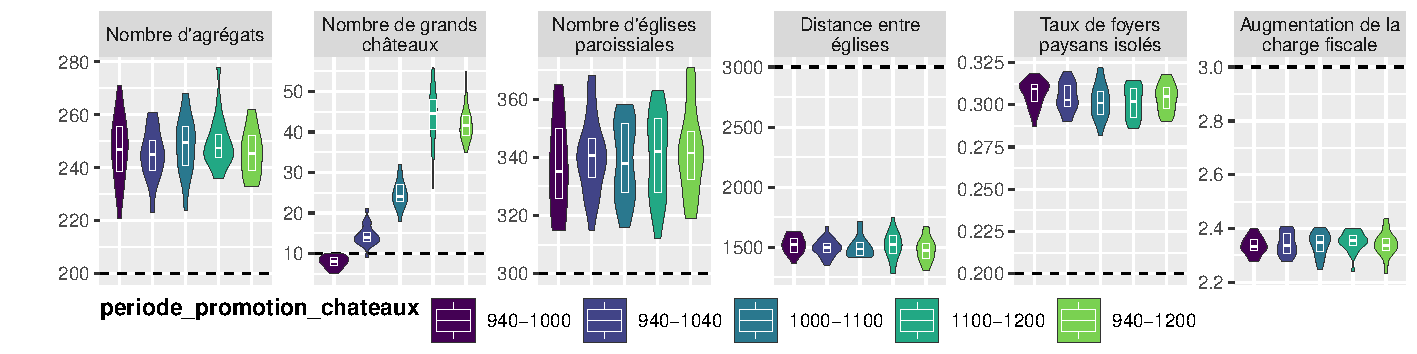
\includegraphics[width=.93\linewidth]{img/sensib/sensibilite_periode_promotion_chateaux.pdf}
	\caption{Sensibilité du paramètre \textsf{periode\_promotion\_chateaux}.}
	\label{fig:sensib-chateaux-1}
\end{figure}

Logiquement, on s'attend à ce que ces paramètres agissent majoritairement sur le seul indicateur numérique lié aux châteaux, ici le nombre de grands châteaux.
C'est bien le cas du paramètre régissant l'intervalle de temps pendant lequel les châteaux peuvent être promus en gros châteaux (\cref{fig:sensib-chateaux-1}).
Ce paramètre semble n'avoir aucun impact sur les autres indicateurs de sortie, mais influence fortement le nombre de gros châteaux.
Sa valeur par défaut (de 940 à 1040, issue de connaissances expertes) est presque optimale au regard de cet indicateur, signe que le calibrage des autres paramètres (moins inscrits dans l'empirie) est adapté.

\begin{figure}[H]
	\centering
	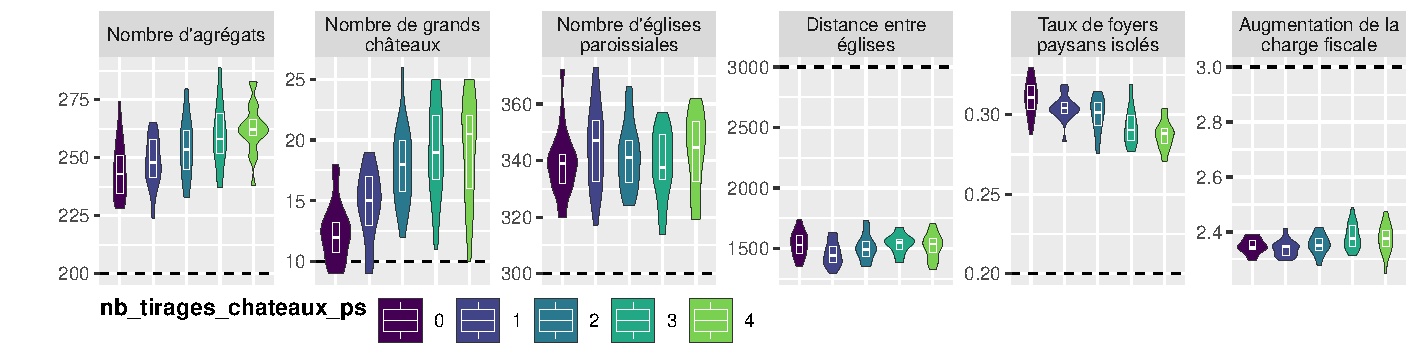
\includegraphics[width=.93\linewidth]{img/sensib/sensibilite_nb_tirages_chateaux_ps.pdf}
	\caption{Sensibilité du paramètre \textsf{nb\_tirages\_chateaux\_ps}.}
	\label{fig:sensib-chateaux-2}
\end{figure}

Les deux autres paramètres liés aux châteaux (\cref{fig:sensib-chateaux-2,fig:sensib-chateaux-3}) ont une influence qui n'est pas circonscrite au nombre de grands châteaux : tous deux agissent sur d'autres indicateurs que celui-ci.

Plus le nombre de tirages probabilistes permettant aux petits seigneurs de construire un château est élevé, plus il y a de grands châteaux en fin de période (\cref{fig:sensib-chateaux-2}), ce qui est attendu au regard des mécanismes.
Par contre, on notera aussi que le nombre de ces châteaux influe sur le nombre d'agrégats et par conséquent sur le taux de foyers paysans isolés :
plus il y a de châteaux, plus il y a de pôles et donc d'agrégats.
Et plus il y a d'agrégats dispersés dans le monde simulé (les châteaux le sont nécessairement puisqu'ils ne peuvent être construits à moins de 5 km les uns des autres), plus les foyers paysans isolés trouvent à migrer localement, diminuant donc la part de ceux qui demeurent isolés en fin de simulation.
Cette influence reste assez modeste toutefois au regard des variations engendrées par le troisième paramètre de cette sélection.

\begin{figure}[H]
	\centering
	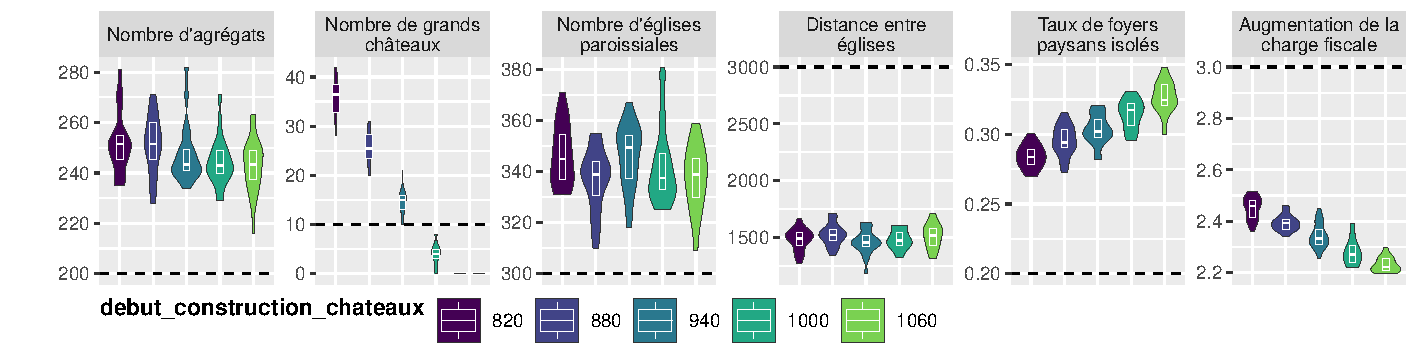
\includegraphics[width=.93\linewidth]{img/sensib/sensibilite_debut_construction_chateaux.pdf}
	\caption{Sensibilité du paramètre \textsf{debut\_construction\_chateaux}.}
	\label{fig:sensib-chateaux-3}
\end{figure}
\clearpage

Celui-ci (\cref{fig:sensib-chateaux-3}) agit de manière assez similaire en termes de tendance, avec une influence plus importante toutefois.
Les figures peuvent laisser penser à une relation inverse à celle du paramètre précédent, mais c'est uniquement dû aux valeurs de ce paramètre qui fixe l'année à partir de laquelle des châteaux peuvent être construits : plus cette année est tardive, moins le nombre de châteaux final sera important\footnote{
	Au contraire du paramètre précédent, où une modalité plus forte impliquait plus de châteaux.
}.
Au-delà des remarques précédentes, on notera que la date de construction des premiers châteaux influe sur l'augmentation de la charge fiscale, dans un sens qui nous semble à nouveau intuitif : plus il y a de châteaux, plus il y a de zones de prélèvement associées, et plus les foyers paysans voient leur charge fiscale augmenter.

De manière générale, la conception et le paramétrage des mécanismes liés aux châteaux ont demandé un travail conséquent (voir la partie dédiée à leur calibrage -- \cref{subsec:calibrage} -- p.~\pageref{subsubsec:calibrage-chateaux}), qui nous a pourtant semblé, lors ces étapes, assez peu convaincant au regard de l'amélioration très modeste que cela a apporté en termes d'ajustement général du modèle.
D'où de nombreux débats internes entre modélisateurs et thématiciens sur la nécessité de détailler autant les mécanismes liés à la construction des châteaux.

L'analyse du premier paramètre (\textsf{periode\_promotion\_chateaux}, \cref{fig:sensib-chateaux-1}) semble aller dans ce sens, puisque la complexité des mécanismes de promotion des châteaux ne semble influencer, sur ces indicateurs très synthétiques, que l'indicateur directement lié : le nombre de gros châteaux.

Les résultats de l'analyse de sensibilité des autres paramètres (\cref{fig:sensib-chateaux-2,fig:sensib-chateaux-3}) donnent tort à l'intuition du modélisateur-\og calibreur\fg{}, et gain de cause aux thématiciens pour lesquels les châteaux, et la justesse de leur implémentation, avaient une dimension thématique considérable.
La portée réduite mais claire de ces paramètres sur le premier objectif thématique recherché (la concentration des foyers paysans) justifie de leur existence et de leur nécessité dans les processus modélisés au sein de \simfeodal{}.

\subsubsection{Paramètres liés aux églises et paroisses\label{sssec:sensib-params-eglises}}

Le dernier paramètre de cette analyse visuelle est aussi le seul qui porte sur les paroisses.
Celles-ci constituent l'un des moteurs principaux de la fixation de la population dans les agrégats de taille réduite qui constituent la grande majorité des lieux de concentration des foyers paysans (la fameuse \og longue traîne\fg{} de cette hiérarchie).
En première analyse, cette sous-représentation des paramètres liés aux paroisses dans l'ensemble des paramètres sélectionnés nous apparaît donc contre-intuitif.

La \cref{fig:sensib-paroisses} présente les réponses des indicateurs à différentes valeurs du paramètre \textsf{ponderation\_creation\_paroisse\_agregat}, qui agit sur le nombre de foyers paysans nécessaires à la création d'une nouvelle église paroissiale au sein des agrégats.
De manière prévisible et évidente, ce paramètre influence nettement les deux indicateurs liés aux paroisses et églises :
plus grand est le nombre de paroissiens nécessaire à la création d'une nouvelle paroisse dans un agrégat, plus faible est le nombre d'églises paroissiales conséquemment créées.
Et moins il y a d'églises dans un monde à la superficie constante, plus large est la distance entre elles.
\clearpage

\begin{figure}[H]
	\centering
	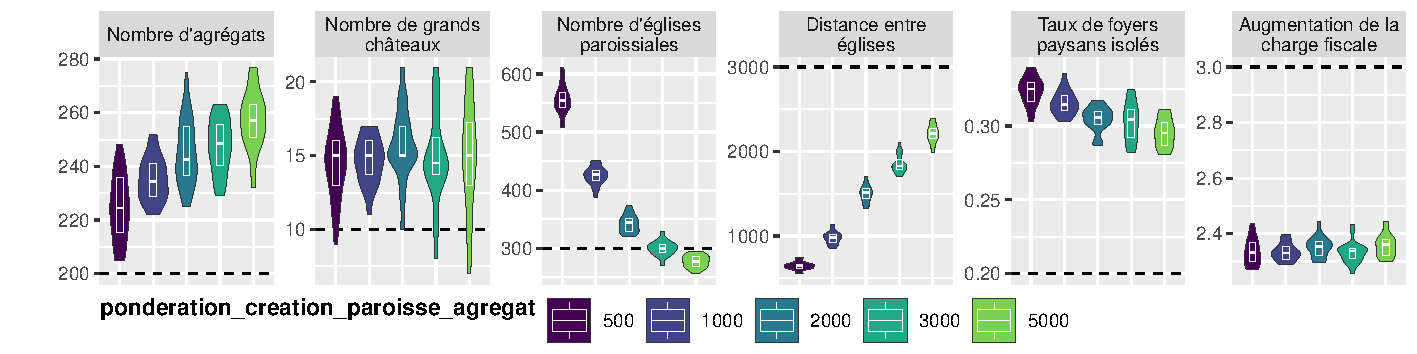
\includegraphics[width=.92\linewidth]{img/sensib/sensibilite_ponderation_creation_paroisse_agregat.pdf}
	\caption{Sensibilité du paramètre de pondération de création de nouvelles paroisses dans les agrégats.}
	\label{fig:sensib-paroisses}\vspace{-.5em}
\end{figure}

Passé ces éléments intuitifs, on notera avec intérêt la variation amenée par ce paramètre sur le nombre d'agrégats : plus le seuil est élevé, plus les agrégats sont nombreux, et cette corrélation apparaît visuellement significative et inverse à celle du nombre d'églises paroissiales.
Cette tendance est inverse à celles observées dans les paramètres liés aux foyers paysans et agrégats (\cref{subsubsec:sensib-fp}, \cref{fig:sensib-fp-1,fig:sensib-fp-2,fig:sensib-fp-3,fig:sensib-agregats}).
Pour ces paramètres, les nombres d'agrégats et d'églises paroissiales varient dans le même sens face à une augmentation de la valeur des paramètres.
Dans le cas du paramètre de pondération de la création de paroisses \og urbaines\fg{}, la relation est inverse (\cref{fig:sensib-paroisses}).

Cela nous paraît contre-intuitif au regard des mécanismes du modèle, et résulte vraisemblablement d'effets inattendus des interactions entre ces mécanismes.
Une piste d'explication réside dans l'influence de ce paramètre de pondération des créations de paroisse sur la hiérarchisation des paroisses et des pôles.
En créant moins de paroisses en zone dense, la distribution de l'attractivité des pôles d'attraction -- qui dépend en large partie du nombre d'églises paroissiales qui les composent -- tend vers plus d'uniformité.
Quand les pôles ont une attractivité plus homogène, les migrations locales sont favorisées, et la concentration s'effectue alors vers des pôles moins attractifs constitués d'agrégats faiblement peuplés.

\vspace{-1em}\subsection{Analyser la sensibilité à l'aléa \label{subsec:sensibilite-alea}}
\vspace{-.5em}En menant l'analyse de sensibilité visuelle, on a pu remarquer que certains indicateurs présentaient une plus forte variation que d'autres.
Une partie de l'explication tient à l'inégale amplitude des valeurs de paramètres testées, mais d'autres facteurs peuvent être en jeu.

De manière globale, on constate dans les résultats de la version calibrée de \simfeodal{} (\cref{tab:results-basique}) que la variabilité des indicateurs émergents, mesurée à partir de leur écart-type, est forte.
L'écart-type se lisant dans l'unité de l'indicateur, il peut être intéressant de le transformer en coefficient de variation ($CV_{\text{indicateur}} = \sigma_{\text{indicateur}} / \mu_{\text{indicateur}}$) pour obtenir des valeurs comparables entre les indicateurs. 

\begin{table}[H]
\vspace{-.5em}
{\small	
{\renewcommand{\arraystretch}{.9}%
	\begin{tabular}{|p{8.25cm}|p{1.75cm}|p{1.9cm}|p{2.25cm}|}
\hline
\textbf{Indicateur} & \textbf{Moyenne} & \textbf{Écart-type} & \textbf{Coefficient de variation} \\
\hline
\textit{Agrégats} & 249 & 10.45 & 0.042\\
\hline
\textit{Grands châteaux} & 15 & 2.87 & 0.191\\
\hline
\textit{Églises paroissiales} & 348 & 12.96 & 0.037\\
\hline
\textit{Distance moyenne entre églises} & 1459 m & 97 m & 0.066\\
\hline
\textit{Part de foyers paysans isolés} & 30\% & 0.8 \% & 0.027\\
\hline
\textit{Augmentation de la charge fiscale des foyers paysans} & $\times$ 2.4 & 0.030 & 0.013\\
\hline
\multicolumn{3}{r|}{\textbf{\textit{Moyenne}}} & 0.063\\
\cline{4-4}
	\end{tabular}}
}
\caption[Dispersion des indicateurs de sortie de \simfeodal{}.]{Dispersion des indicateurs de sortie de la version calibrée (6.6) de \simfeodal{}.}
\label{tab:variabilite-indicateurs}
\end{table}
\clearpage

La comparaison des coefficients de variation \cref{tab:variabilite-indicateurs} montre que la variabilité des indicateurs due à l'aléa est assez faible, et d'ordre de grandeurs comparables d'un indicateur à l'autre\footnote{
	Le nombre de grands châteaux fait exception : son coefficient de variation (0.191) est nettement supérieur aux autres.
	Cela s'explique par l'ordre de grandeur du nombre de châteaux et grands châteaux, faible relativement aux autres, et où des variations de quelques unités jouent beaucoup sur l'écart-type en raison de la nature entière de ces variables.
}.

Pourtant, lors de l'analyse de sensibilité, on a pu constater des variations (étendue dans l'axe des ordonnées des \textit{violin-plots}) bien différentes au sein des réplications des paramètres testés.
Dans la \cref{fig:sensib-fp-2} par exemple, on peut remarquer que la modalité \og dynamique\_large\fg{} présente une variabilité à l'aléa (le \og violon\fg{} est très étendu) différente des autres modalités : plus faible sur le nombre d'églises paroissiales et plus importante sur l'augmentation de la charge fiscale.
De même, l'indicateur \textsf{ponderation\_creation\_paroisse\_agregat} (\cref{fig:sensib-paroisses}) présentait, sur le nombre de grands châteaux, une importante différence de variabilité à l'aléa.

Il nous paraît par conséquent utile de mener un bref complément d'analyse, dédié à l'étude de la variabilité au sein des réplications d'une expérience.
De telles analyses systématiques nous paraissent peu fréquentes dans la littérature liée aux modèles de simulation en géographie.
On trouve une définition de ce type d'approche chez \textcite{ginot2005explorer}, sous le terme d'\og analyses d'incertitude\fg{} : 
\begin{quotation}
	\og Compte tenu des incertitudes sur les paramètres, de la variabilité naturelle des variables d'entrée et des composantes stochastiques qui peuvent être incluses dans la structure du modèle, il s'agit de calculer l'incertitude associée aux variables de sorties.
	Les analyses d'incertitude sont très liées aux analyses de sensibilité dans la mesure où l'on souhaite en général connaître non seulement cette incertitude, mais également son origine.
	C'est pourquoi ces deux types d'analyses sont souvent menées en parallèle, voire confondues.\fg{}\\
	\mbox{}~ \hfill \cite[76]{ginot2005explorer}
\end{quotation}

Pour mesurer cette incertitude, nous avons repris l'ensemble des réplications correspondant à l'analyse de sensibilité de chaque paramètre et avons mesuré la variabilité (écart-type) sur chaque indicateur.
Afin d'avoir des mesures comparables, on a ensuite procédé à une réduction (division par l'écart-type des valeurs de référence, présentées dans le \cref{tab:variabilite-indicateurs}) de l'amplitude de ces valeurs.

La distribution de ces valeurs d'incertitude relatives est présenté dans la \cref{fig:histo-sensib-alea}.
Dans ces histogrammes, la valeur de 1 correspond à une incertitude moyenne identique à celle des réplications de référence, c'est-à-dire des réplications de la version calibrée du modèle dont les résultats ont été commentés dans la première partie de ce chapitre (\cref{subsec:resultats}).
Une valeur de 2 peut être comprise ainsi : pour l'indicateur considéré, les différentes simulations exécutées lors de l'analyse de chaque valeur de chaque paramètre ont une variabilité deux fois supérieure à la variabilité de référence.
Autrement dit, certaines valeurs de certains paramètres amènent une bien plus forte variabilité : ils laissent une part plus importante à la stochasticité du modèle.

\begin{figure}[H]
	\centering
	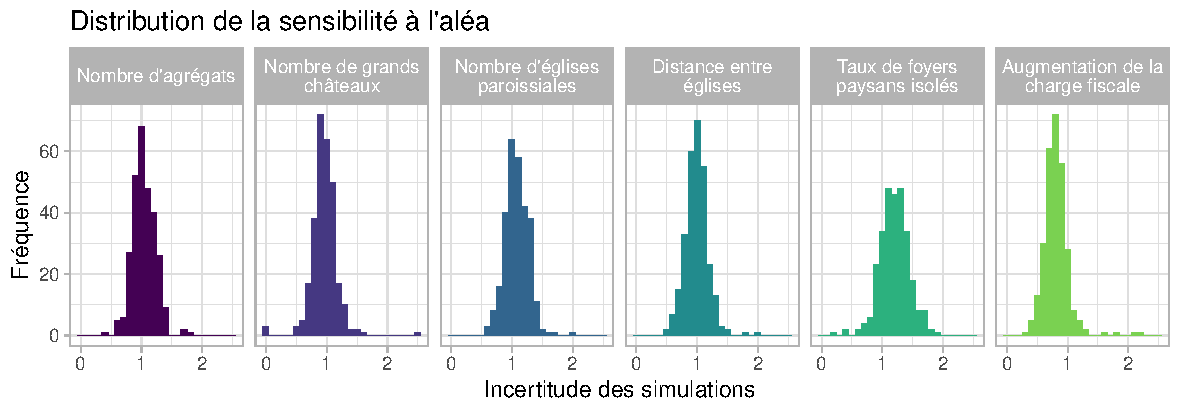
\includegraphics[width=\linewidth]{img/histo_sensibilite_alea.pdf}
	\caption[Sensibilité à l'aléa selon les indicateurs.]{Sensibilité à l'aléa selon les indicateurs.\\
	{\small
	\textit{L'incertitude mesurée se lit en proportion de l'écart-type des résultats de la version calibrée de \simfeodal{}.
	Une valeur de 0.5, par exemple, signifie que la variabilité due à l'aléa est moitié moins importante	que celle des valeurs de paramètres issues du calibrage.}}}
	\label{fig:histo-sensib-alea}
\end{figure}

On peut remarquer que la plupart des indicateurs présentent des \textit{outliers}, c'est-à-dire des valeurs de paramètres pour lesquelles la variabilité due à l'aléa est nettement supérieure (ou inférieure) à la normale.
Dans le cas du nombre de grands châteaux, il y a même des valeurs de paramètres qui montre une absence presque totale de variabilité à l'aléa.
Sans aller plus loin sur cet exemple, il s'agit en fait des valeurs de paramètre qui ont tendance à réduire très largement le nombre de châteaux, amenant alors à une variabilité extrêmement faible dans cette amplitude des possibles restreinte.

À partir de cet histogramme, nous avons isolés les \textit{outliers} et en proposons une représentation graphique dans la \cref{fig:sensib-alea}.
\begin{figure}[H]
	\centering
	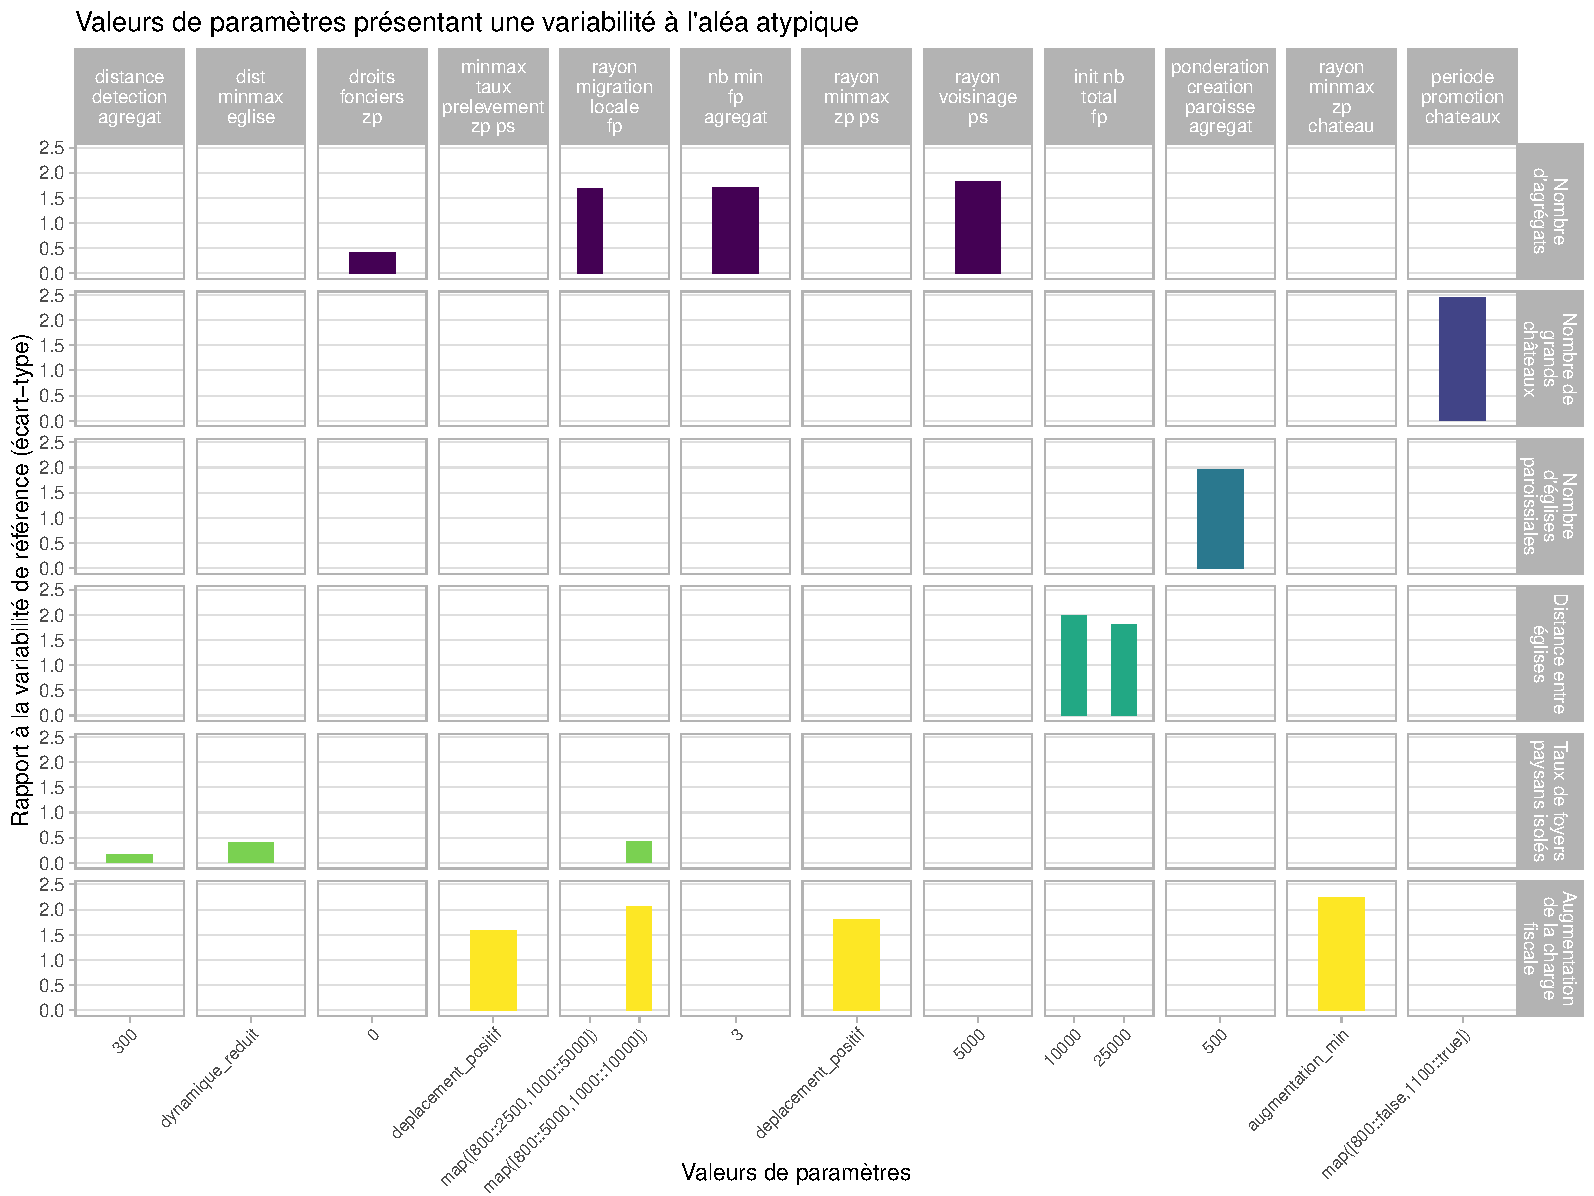
\includegraphics[width=.95\linewidth]{img/sensibilite_alea_outliers.pdf}
	\caption{Paramètres présentant des sensibilités atypiques à l'aléa.}
	\label{fig:sensib-alea}
\end{figure}
\clearpage

De manière globale, on peut remarquer que les indicateurs relatifs aux foyers paysans (Nombre d'agrégats, taux de foyers paysans isolés et augmentation de la charge fiscale) sont surreprésentés parmi cette sélection d'\textit{outliers}.
Cela montre bien que les foyers paysans sont les agents qui subissent le plus les changements de valeurs des paramètres du modèle.

Notons aussi que sur les 14 \textit{outliers} identifiés (axe des abscisses), la moitié sont des valeurs de paramètres qualitatifs.
La difficile estimation de l'amplitude de ceux-ci explique sans doute en partie la plus forte variabilité à l'aléa : si on choisit des valeurs (étendues, évolutions temporelles etc.) trop éloignées des valeurs calibrées, il se peut que le modèle réagisse de manière non habituelle aux interactions entre mécanismes.

Plus spécifiquement, on peut constater le comportement très particulier du paramètre régissant le rayon maximum de migration locale des foyers paysans (\textsf{rayon\_migration\_locale\_fp}, cinquième colonne en partant de la gauche dans la \cref{fig:sensib-alea}).
Certaines valeurs de ce paramètre sont parmi les plus sensibles à l'aléa (notamment sur le nombre d'agrégats et l'augmentation de la charge fiscale : les barres y sont parmi les plus élevées de la figure).
De plus, de manière surprenante, la valeur correspondant à un rayon évolutif très étendu (\texttt{map([800:5000, 1000:10000])}) se caractérise aussi par une très faible sensibilité à l'aléa sur l'indicateur de concentration des foyers paysans.

Ce paramètre a donc la capacité de faire fortement varier les sorties (vu dans l'analyse de sensibilité visuelle), mais en plus de faire varier tout aussi fortement la part de l'aléa dans le modèle, en la diminuant ou en l'augmentant.
%Nous pensions exécuter un scénario thématique qui fasse varier ce paramètre afin d'étudier l'effet sur la hiérarchie des agrégats, et cette analyse confirme que ce serait tout à faire approprié.

\subsection{Quels apports de l'analyse visuelle de sensibilité ?\label{subsec:apports-analyse-visuelle-sensib}}

En dépit de certaines limites que nous avons détaillées, cette analyse de sensibilité a permis de mettre en évidence un certain nombre de propriétés des paramètres et d'apporter des connaissances extrêmement utiles sur le fonctionnement du modèle face à divers types d'aléas en particulier.

Premièrement, notons que la hiérarchie de la sensibilité des paramètres diffère de celle que l'on attendait.
Le paramétrage et le calibrage ont ainsi été menés, en partie, sur des paramètres moins déterminants que notre intuition du comportement du modèle ne pouvait le laisser croire.
Cette étape d'évaluation qu'est l'analyse de sensibilité gagnerait à être menée avant le calibrage du modèle afin d'obtenir une meilleure adéquation aux objectifs.
Ce raisonnement est toutefois circulaire : sur un modèle moins calibré, l'analyse de sensibilité n'aurait pas forcément mis en avant les mêmes paramètres.
Comme ceux-si sont en interaction étroite, les résultats de cette analyse de sensibilité sont ainsi, eux-mêmes, extrêmement sensibles au paramétrage de base.

Ensuite, l'analyse de sensibilité semble confirmer que le modèle est parcimonieux, relativement à sa nature exploratoire du moins.
On l'a dit lors de l'analyse quantitative, mais il nous semble important de le répéter tant ce résultat est rassurant au regard des craintes que l'on pouvait avoir : quand un modèle implique autant de mécanismes et paramètres, le risque est toujours important que certains soient redondants et donc superflus.
Aucun des paramètres n'apparaît inutile, ce qui peut laisser entendre que les (très) nombreux mécanismes du modèle ne le sont pas non plus.
Pour un modélisateur qui a des intuitions fortes sur les réactions d'un modèle aux différents changements de mécanismes et paramètres, cela constitue une surprise.
Surprise d'autant plus positive que cet examen systématique des paramètres se révèle réellement une aide indéniable à la compréhension du modèle.
Après plus de 5 ans à travailler régulièrement sur un modèle, il est très enrichissant d'y trouver encore des éléments inattendus voir nettement contre-intuitifs.
De ce fait, l'analyse de sensibilité favorise elle aussi l'abduction (voir \cref{subsec:depasser-calibrage}).

Un autre point, classique, concerne les limites d'une telle analyse.
Une approche entièrement quantitative, présentée dans l'introduction de cette partie, permet de s'affranchir des effets de faible comparabilité que l'on a pu constater dans l'analyse visuelle : certains paramètres ont une sensibilité globale importante, mais celle-ci se cantonne parfois à un unique indicateur, sans avoir de répercussions sur le reste du modèle.
Un modèle comme \simfeodal{}, c'est-à-dire descriptif, exploratoire, est caractérisé par des paramètres nombreux, hétérogènes et parfois très qualitatifs.
Il ne serait pas pertinent de chercher à quantifier, uniquement pour mener une analyse de sensibilité, tout ce qui n'a pas été quantifié dans le modèle en lui-même : objectivation des attendus dans les indicateurs graphiques, quantification de la pondération entre les différents objectifs etc.

La démarche mise en place pour cette analyse de sensibilité a été basée sur une volonté d'exploration graphique et s'inscrit, comme de nombreux aspects de ce travail de thèse, dans une approche d'analyse visuelle entièrement dédiée à l'exploration d'un modèle.
Cette démarche paraît confirmer l'adéquation de ce type d'approches à la construction et à l'évaluation commune et interdisciplinaire de modèles.
Les éléments de compréhension des interactions effectives du modèle et les retours auxquels ces découvertes incitent nous paraissent entièrement fructueux, et à mettre au crédit de cette approche exploratoire, visuelle, et fondamentalement très qualitative.

\section*{Conclusion}
\addcontentsline{toc}{section}{\protect\numberline{}Conclusion}

Dans ce chapitre, nous avons présenté les dernières étapes de calibrage de \simfeodal{} et les résultats qui en émanent.
À l'aune de ces résultats, on peut conclure que le modèle, une fois calibré, est globalement satisfaisant, sur chacune des dimensions d'objectifs poursuivis : concentration et polarisation, hiérarchisation et fixation-dissémination du peuplement.
L'ajustement n'est certes jamais parfait, mais aussi bien en termes de valeurs btenues que d'évolutions de ces valeurs au cours du paramétrage et du calibrage du modèle, cet ajustement nous apparaît tout à fait satisfaisant.

Dans la seconde partie de ce chapitre, nous partions du constat qu'il est difficile d'améliorer le calibrage du modèle à cause des effets d'interactions et des réponses inattendues de certains paramètres.
Pour y remédier, nous avons mené une analyse de sensibilité de l'ensemble des paramètres de \simfeodal{} qui nous a permis de mieux comprendre l'influence de chaque paramètre et mécanisme lié sur les sorties du modèle.
Cette analyse de sensibilité a aussi contribué à isoler certains paramètres qui constitueraient des leviers sur lesquels agir pour améliorer le calibrage du modèle : des paramètres sans effets de bord, qui n'agissent véritablement que sur les indicateurs auxquels ils sont directement liés.

L'analyse de sensibilité a aussi débouché sur l'identification de paramètres ayant une influence plus importante que nous ne le pensions, voir une influence inverse, de manière contre-intuitive.
Ces paramètres, entre autres, nous semblent de très bons candidats à la réalisation de scénarios thématiques (voir \cref{enc:scenario-croissance-demo}) qui permettraient de comprendre les répercussions thématiques de ces résultats simulés surprenants.

Un élément limite pourtant fortement d'éventuelles améliorations et exploitations plus fines des résultats du modèle : le risque d'\textit{overfitting}.
Au vu de la précision faible et hétérogène des connaissances empiriques par le prisme desquelles \simfeodal{} est évalué, il paraît difficile de chercher à comparer de nouvelles versions du modèle dont les variations sur les indicateurs sont de plus en plus fines à mesure que le calibrage progresse.

Cela n'empêche aucunement le modèle d'être utile, utilisable et utilisé.
Nous n'avons présenté qu'un des scénarios sur la quinzaine réalisée, mais celui-ci apporte déjà beaucoup de matière à réflexion, autant d'un point de vue restreint au modèle que, plus généralement, sur les processus thématiques que \simfeodal{} cherche à reproduire.

Dans l'ensemble, la calibration, l'analyse de sensibilité et les scénarios servent certes un rôle de validation interne, mais surtout, ils permettent aux co-concepteurs du modèle de mieux en comprendre les biais et le fonctionnement effectif, c'est-à-dire issu des innombrables interactions entre mécanismes.
Afin de saisir les effets contre-intuitifs liés à ces interactions, c'est-à-dire en cherchant à acquérir une connaissance plus intime du modèle, on effectue un travail dont les apports thématiques sont certains.
Comme dans la conception d'un modèle, l'analyse de ses résultats et la recherche de leur amélioration force ainsi les modélisateurs à mieux formaliser et expliciter les hypothèses et attentes sous-jacentes.
Dans le cadre d'un modèle dédié à l'étude de processus anciens sur le temps long, ces différentes phases ont aussi poussé à la recherche approfondie de nouvelles sources et documentations sur les faits stylisés et mécanismes implémentés dans le modèle.
Toutes ces étapes, loin de viser à une validation théorique du modèle, sont ainsi autant d'occasions d'échanger et de co-construire des connaissances toujours plus formalisées.
Il nous semble que c'est là l'enjeu majeur de cette expérience de construction collective et interdisciplinaire d'un modèle exploratoire.
